% =====================================================================
% Tesis -- Neuromorphic Lab
% Simulador Modular de Memristores y Circuitos Neuromórficos
% =====================================================================
\documentclass[11pt,a4paper,oneside]{book}

% --- Codificación e idioma ---
\usepackage[utf8]{inputenc}
\usepackage[T1]{fontenc}
\usepackage[spanish,es-tabla]{babel}

% --- Matemáticas ---
\usepackage{amsmath}
\usepackage{amssymb}
\usepackage{bm}

% --- Figuras y tablas ---
\usepackage{graphicx}
\usepackage{float}
\usepackage[singlelinecheck=false]{caption}
\usepackage{subcaption}
\usepackage{booktabs}
\usepackage{array}
\usepackage{longtable}

% --- Hipervínculos y colores ---
\usepackage[hidelinks]{hyperref}
\usepackage{xcolor}

% --- Bibliografía ---
\usepackage{cite}

% --- Espaciado y márgenes ---
\usepackage{setspace}
\onehalfspacing
\usepackage{geometry}
\geometry{margin=2.5cm}

% --- Comandos auxiliares ---
\newcommand{\Rtwo}{R^{2}}
\newcommand{\ISI}{\mathrm{ISI}}
\newcommand{\RON}{R_{\mathrm{ON}}}
\newcommand{\ROFF}{R_{\mathrm{OFF}}}
\newcommand{\Robj}{R_{\mathrm{obj}}}
\newcommand{\Rteo}{R_{\mathrm{teo}}}

% --- Metadatos ---
\title{\textbf{Neuromorphic Lab: Simulador Modular de Memristores y Circuitos Neuromórficos}\\[0.5em]
\Large Tesis de Grado -- Validación Cuantitativa y Arquitectura Hardware}
\author{\textbf{Yamil Uchani}}
\date{\today}

\begin{document}

\frontmatter
\maketitle
\tableofcontents
\listoffigures
\listoftables

\chapter*{Resumen}
\addcontentsline{toc}{chapter}{Resumen}
Este documento presenta la validación cuantitativa y cualitativa del simulador Neuromorphic Lab, una plataforma modular diseñada para el estudio de dispositivos memristivos y arquitecturas neuromórficas. El desarrollo se dividió en cuatro fases: modelado de la celda unitaria de Strukov, integración híbrida con neuronas Leaky Integrate-and-Fire (LIF), implementación de plasticidad sináptica (STDP, LTP/LTD) y escalamiento a matrices In-Memory Computing (Crossbar). Los resultados demuestran una altísima correlación ($R^2 > 0.93$) con datos empíricos de literatura científica de referencia (Strukov 2008, Jo 2010, Prezioso 2015, Wang 2025), validando la viabilidad del simulador como herramienta rigurosa para la investigación en hardware neuromórfico, logrando reproducir fielmente fenómenos de variabilidad estocástica, asimetría de conmutación y computación paralela analógica.

\chapter*{Nomenclatura y Acrónimos}
\addcontentsline{toc}{chapter}{Nomenclatura y Acrónimos}
\section*{Acrónimos}
\begin{itemize}
    \item \textbf{C2C}: Cycle-to-Cycle (Variabilidad ciclo a ciclo)
    \item \textbf{D2D}: Device-to-Device (Variabilidad dispositivo a dispositivo)
    \item \textbf{ISI}: Inter-Spike Interval (Intervalo entre pulsos)
    \item \textbf{LIF}: Leaky Integrate-and-Fire (Modelo neuronal)
    \item \textbf{LTD}: Long-Term Depression (Depresión a largo plazo)
    \item \textbf{LTP}: Long-Term Potentiation (Potenciación a largo plazo)
    \item \textbf{STDP}: Spike-Timing-Dependent Plasticity (Plasticidad dependiente del tiempo)
    \item \textbf{VMM}: Vector-Matrix Multiplication (Multiplicación vector-matriz)
\end{itemize}

\section*{Símbolos}
\begin{itemize}
    \item $G$: Conductancia ($\Omega^{-1}$ o Siemens)
    \item $R_S$: Resistencia en serie ($\Omega$)
    \item $V_{th}$: Voltaje de umbral (V)
    \item $x$: Variable de estado interna (adimensional o nm)
    \item $w$: Ancho de la región dopada (nm)
    \item $D$: Espesor total del dispositivo (nm)
\end{itemize}

\newpage

\mainmatter

% --- Capítulos principales ---
% =====================================================================
% Capítulo 1: Introducción
% =====================================================================

\chapter{Introducción}
\label{ch:introduccion}

\section{Contexto y motivación}
\label{sec:intro-contexto}

El crecimiento exponencial de las aplicaciones de inteligencia artificial y procesamiento de datos ha puesto en evidencia las limitaciones intrínsecas de la arquitectura computacional von Neumann tradicional. La separación física entre las unidades de procesamiento central (CPU/GPU) y las memorias secundarias genera un cuello de botella de ancho de banda y un consumo energético insostenible, conocido como el \emph{cuello de botella de von Neumann}.

La computación neuromórfica surge como una alternativa paradigmática inspirada en la arquitectura y dinámica de los sistemas biológicos cerebrales. Al integrar la memoria y el procesamiento en el mismo elemento físico mediante redes de memristores y neuronas artificiales tipo Disparo e Integración con Fuga (\emph{Leaky Integrate-and-Fire}, LIF), es posible reducir el consumo energético en varios órdenes de magnitud y habilitar el aprendizaje en tiempo real en dispositivos de borde (\emph{edge computing}).

\section{Planteamiento del problema}
\label{sec:intro-problema}

A pesar de los avances teóricos en dispositivos memristivos y modelos de neuronas de impulsos (\emph{spiking neurons}), existe una brecha significativa entre la modelación analítica aislada y las plataformas de simulación de circuitos completos integrados. Los simuladores existentes frecuentemente presentan uno o más de los siguientes inconvenientes:
\begin{enumerate}
    \item Falta de modularidad para intercambiar dinámicamente modelos de memristores no volátiles (Strukov, Prezioso, Jo) y volátiles (Wang, Yang).
    \item Omisión de efectos no ideales deterministas y estocásticos reales, como la variabilidad dispositivo a dispositivo (\emph{device-to-device}, D2D) y ciclo a ciclo (\emph{cycle-to-cycle}, C2C).
    \item Dificultad para validar de forma automatizada y reproducible la precisión numérica frente a datos experimentales publicados en la literatura.
\end{enumerate}

\section{Objetivos}
\label{sec:intro-objetivos}

\subsection{Objetivo general}
Desarrollar y validar cuantitativamente una plataforma de simulación modular en Python (\emph{Neuromorphic Lab}) para la modelación y análisis de dispositivos memristivos, neuronas LIF, circuitos híbridos y matrices de interconexión (\emph{crossbar array}), con interfaz gráfica interactiva y verificación automatizada contra datos de la literatura.

\subsection{Objetivos específicos}
\begin{enumerate}
    \item Implementar una biblioteca centralizada de modelos físicos y matemáticos de memristores (Strukov, Yakopcic/Prezioso, Jo, Wang) y neuronas LIF.
    \item Incorporar variabilidad estocástica D2D y C2C mediante distribuciones normales truncadas y procesos de Ornstein-Uhlenbeck.
    \item Diseñar e integrar algoritmos de plasticidad sináptica Hebbiana (\emph{Spike-Timing-Dependent Plasticity}, STDP) y reforzada (\emph{R-STDP}).
    \item Consolidar la arquitectura de matrices crossbar (1×1, 2×2, 4×4) en una implementación unificada con decodificadores y controladores de fila/columna.
    \item Construir una suite de 27 pruebas de validación automatizadas reportando métricas de precisión ($\text{MAE}$, $\text{RMSE}$, $\text{Error Relativo}$ y $R^2$).
\end{enumerate}

% =====================================================================
% Capítulo 2: Marco Teórico
% =====================================================================

\chapter{Marco Teórico}
\label{ch:marco-teorico}

\section{Fundamentos del Memristor}
\label{sec:marco-memristor}

El memristor (\emph{memory resistor}), postulado hipotéticamente por Leon Chua en 1971 como el cuarto elemento pasivo fundamental de circuito y sintetizado por primera vez en laboratorios de HP por Strukov et al. en 2008~\cite{strukov2008}, establece una relación directa entre la carga eléctrica acumulada $q$ y el flujo magnético $\varphi$:

\begin{equation}
d\varphi = M(q) \, dq
\label{eq:memristor-fundamental}
\end{equation}

La resistencia equivalente del dispositivo, denominada \emph{memristancia} $M(w)$, depende dinámicamente de una variable interna de estado $x(t) = w(t)/D \in [0, 1]$, que representa la frontera física entre la zona dopada y no dopada del material.

\subsection{Modelo matemático de Strukov (2008)}
\label{subsec:marco-strukov}

En el modelo de Strukov et al.~\cite{strukov2008}, la resistencia total $R(x)$ se expresa como una combinación lineal estricta de las resistencias extremas en estado ON ($\RON$) y OFF ($\ROFF$):

\begin{equation}
R(x) = \RON \cdot x + \ROFF \cdot (1 - x)
\label{eq:strukov-rx}
\end{equation}

La ecuación diferencial de evolución del estado interno $x(t)$ bajo una corriente $i(t)$ es:

\begin{equation}
\frac{dx}{dt} = \mu_v \cdot \frac{\RON}{D^2} \cdot i(t) \cdot f(x)
\label{eq:strukov-dxdt}
\end{equation}

donde $\mu_v$ es la movilidad promedio de vacancias de oxígeno y $f(x)$ representa una función de ventana que modela los efectos de frontera no lineales en las interfaces del dispositivo.

\subsection{Modelo de Yakopcic y Prezioso (2011, 2014, 2015)}
\label{subsec:marco-yakopcic}

Para capturar la asimetría umbral y la no linealidad en dispositivos de capa fina $\mathrm{Al_2O_3/TiO_{2-x}}$~\cite{prezioso2014, prezioso2015}, se emplea la formulación de Yakopcic et al.~\cite{yakopcic2011}. La corriente $I(v, x)$ sigue una relación exponencial con el voltaje aplicado $v(t)$:

\begin{equation}
I(v, x) = 
\begin{cases}
a_1 \cdot x(t) \cdot \sinh(b \cdot v(t)), & v(t) \geq 0 \\
a_2 \cdot x(t) \cdot \sinh(b \cdot v(t)), & v(t) < 0
\end{cases}
\label{eq:yakopcic-iv}
\end{equation}

donde la tasa de variación $\dot{x}(t)$ se activa únicamente al superar los voltajes umbrales de SET ($V_p$) y RESET ($V_n$):

\begin{equation}
\frac{dx}{dt} = 
\begin{cases}
A_p \cdot \left( e^{v(t) - V_p} - 1 \right) \cdot f(x), & v(t) > V_p \\
-A_n \cdot \left( e^{-v(t) - V_n} - 1 \right) \cdot f(x), & v(t) < -V_n \\
0, & -V_n \leq v(t) \leq V_p
\end{cases}
\label{eq:yakopcic-dxdt}
\end{equation}

\subsection{Memristores volátiles para nodos sensoriales}
\label{subsec:marco-volatile}

A diferencia de las celdas no volátiles, los memristores volátiles (basados en $\mathrm{HfO_2}$ o nanoclústeres difusivos de $\mathrm{Ag:SiO_2}$)~\cite{wang2025, yang2017} exhiben un fenómeno de relajación espontánea del estado interno hacia un valor basal $x_0$ debido al decaimiento térmico de las filamentaciones metálicas. La cinética de estado se modela mediante:

\begin{equation}
\frac{dx}{dt} = f_{\text{activación}}(v, x) - \frac{x(t) - x_0}{\tau_{\mathrm{relax}}}
\label{eq:volatile-dxdt}
\end{equation}

donde $\tau_{\mathrm{relax}}$ determina la constante de tiempo de olvido o relajación espontánea.

\section{Modelo de Neurona Spiking LIF}
\label{sec:marco-lif}

La neurona de disparo e integración con fuga (\emph{Leaky Integrate-and-Fire}, LIF) constituye el bloque computacional primario en redes neuromórficas. El potencial de membrana $V_m(t)$ evoluciona según la ecuación diferencial:

\begin{equation}
C_m \frac{dV_m(t)}{dt} = I_{\mathrm{syn}}(t) - \frac{V_m(t) - V_{\mathrm{rest}}}{R_{\mathrm{leak}}}
\label{eq:lif-diffeq}
\end{equation}

Cuando el potencial $V_m(t)$ alcanza el umbral de disparo $V_{\mathrm{th}}$, la neurona emite un impulso (\emph{spike}), reinicia su potencial a $V_{\mathrm{reset}}$ y permanece inactiva durante un período refractario $t_{\mathrm{ref}}$:

\begin{equation}
\text{Si } V_m(t) \ge V_{\mathrm{th}} \implies 
\begin{cases}
S(t) = 1 \\
V_m(t^+) = V_{\mathrm{reset}}
\end{cases}
\label{eq:lif-spike}
\end{equation}

\section{Plasticidad Sináptica}
\label{sec:marco-plasticidad}

\subsection{Plasticidad dependiente del tiempo de disparo (STDP)}
\label{subsec:marco-stdp}

La regla de aprendizaje Hebbiano STDP~\cite{bi1998, jo2010} modifica la conductancia sináptica $G_{ij}$ de acuerdo a la diferencia de tiempos $\Delta t = t_{\mathrm{post}} - t_{\mathrm{pre}}$ entre los impulsos pre y postsinápticos:

\begin{equation}
\Delta G = 
\begin{cases}
A_+ \cdot \exp\left( -\frac{\Delta t}{\tau_+} \right), & \Delta t > 0 \quad (\text{Potenciación - LTP}) \\
-A_- \cdot \exp\left( \frac{\Delta t}{\tau_-} \right), & \Delta t < 0 \quad (\text{Depresión - LTD})
\end{cases}
\label{eq:stdp-window}
\end{equation}

\subsection{Plasticidad modulada por recompensa (R-STDP)}
\label{subsec:marco-rstdp}

En sistemas de aprendizaje por refuerzo, la modificación del peso sináptico se modula mediante una señal escalar de recompensa $R(t)$ emitida por el entorno:

\begin{equation}
\frac{dG_{ij}}{dt} = \eta \cdot R(t) \cdot e_{ij}(t)
\label{eq:rstdp-rule}
\end{equation}



donde $e_{ij}(t)$ representa la traza de elegibilidad acumulada producida por los emparejamientos STDP locales.

% =====================================================================
% Capítulo 3: Fase 1
% =====================================================================

\chapter{Fase 1: Núcleo del Dispositivo Memristivo y Variabilidad}
\label{ch:fase1}

Este capítulo detalla la primera fase del proyecto, enfocada en la construcción desde cero de la física del dispositivo memristivo y su variabilidad intrínseca. Se aborda la implementación teórica y cualitativa, culminando con una validación cuantitativa rigurosa contra los modelos seminales de la literatura científica.

% =====================================================================
\section{Etapa 1.1: Modelo Base y Curvas Características}
\label{sec:etapa1_1}

\subsection{Implementación Cualitativa y Fundamentos Físicos}
El núcleo de la simulación recae en el modelo físico del memristor. Para modelar el comportamiento ideal de dispositivos de dióxido de titanio (TiO$_2$), se implementó el modelo fenomenológico de Strukov et al. (2008)~\cite{strukov2008}. El dispositivo se concibe como dos resistencias variables en serie, dependientes de la anchura del filamento conductor $w(t)$ respecto a la longitud total $D$.

La dinámica del estado interno $x(t) = w(t)/D \in [0,1]$ está gobernada por la movilidad iónica $\mu_v$:
\begin{equation}
\frac{dx}{dt} = \frac{\mu_v R_{\mathrm{ON}}}{D^2} i(t) \cdot f_w(x)
\label{eq:strukov_dinamica}
\end{equation}

donde $f_w(x)$ es una función ventana (e.g., Joglekar o Biolek) que impone condiciones de contorno rígidas en los extremos $x=0$ y $x=1$ para evitar singularidades matemáticas. La resistencia total del dispositivo en cada instante es la combinación lineal convexa de sus límites resistivos:
\begin{equation}
R(x) = R_{\mathrm{ON}} x + R_{\mathrm{OFF}} (1-x)
\label{eq:resistencia_lineal}
\end{equation}

La respuesta cualitativa del modelo de Strukov exhibe el clásico lazo de histéresis I-V pinzado en el origen. Al aplicar voltajes periódicos, la conductancia oscila suavemente acotada por los límites $R_{\mathrm{ON}}$ y $R_{\mathrm{OFF}}$. El estado interno $x(t)$ se restringe estrictamente al rango sin saturaciones espurias, comprobable ante señales triangulares continuas (Figura~\ref{fig:val-triangular}).

\begin{figure}[H]
    \centering
    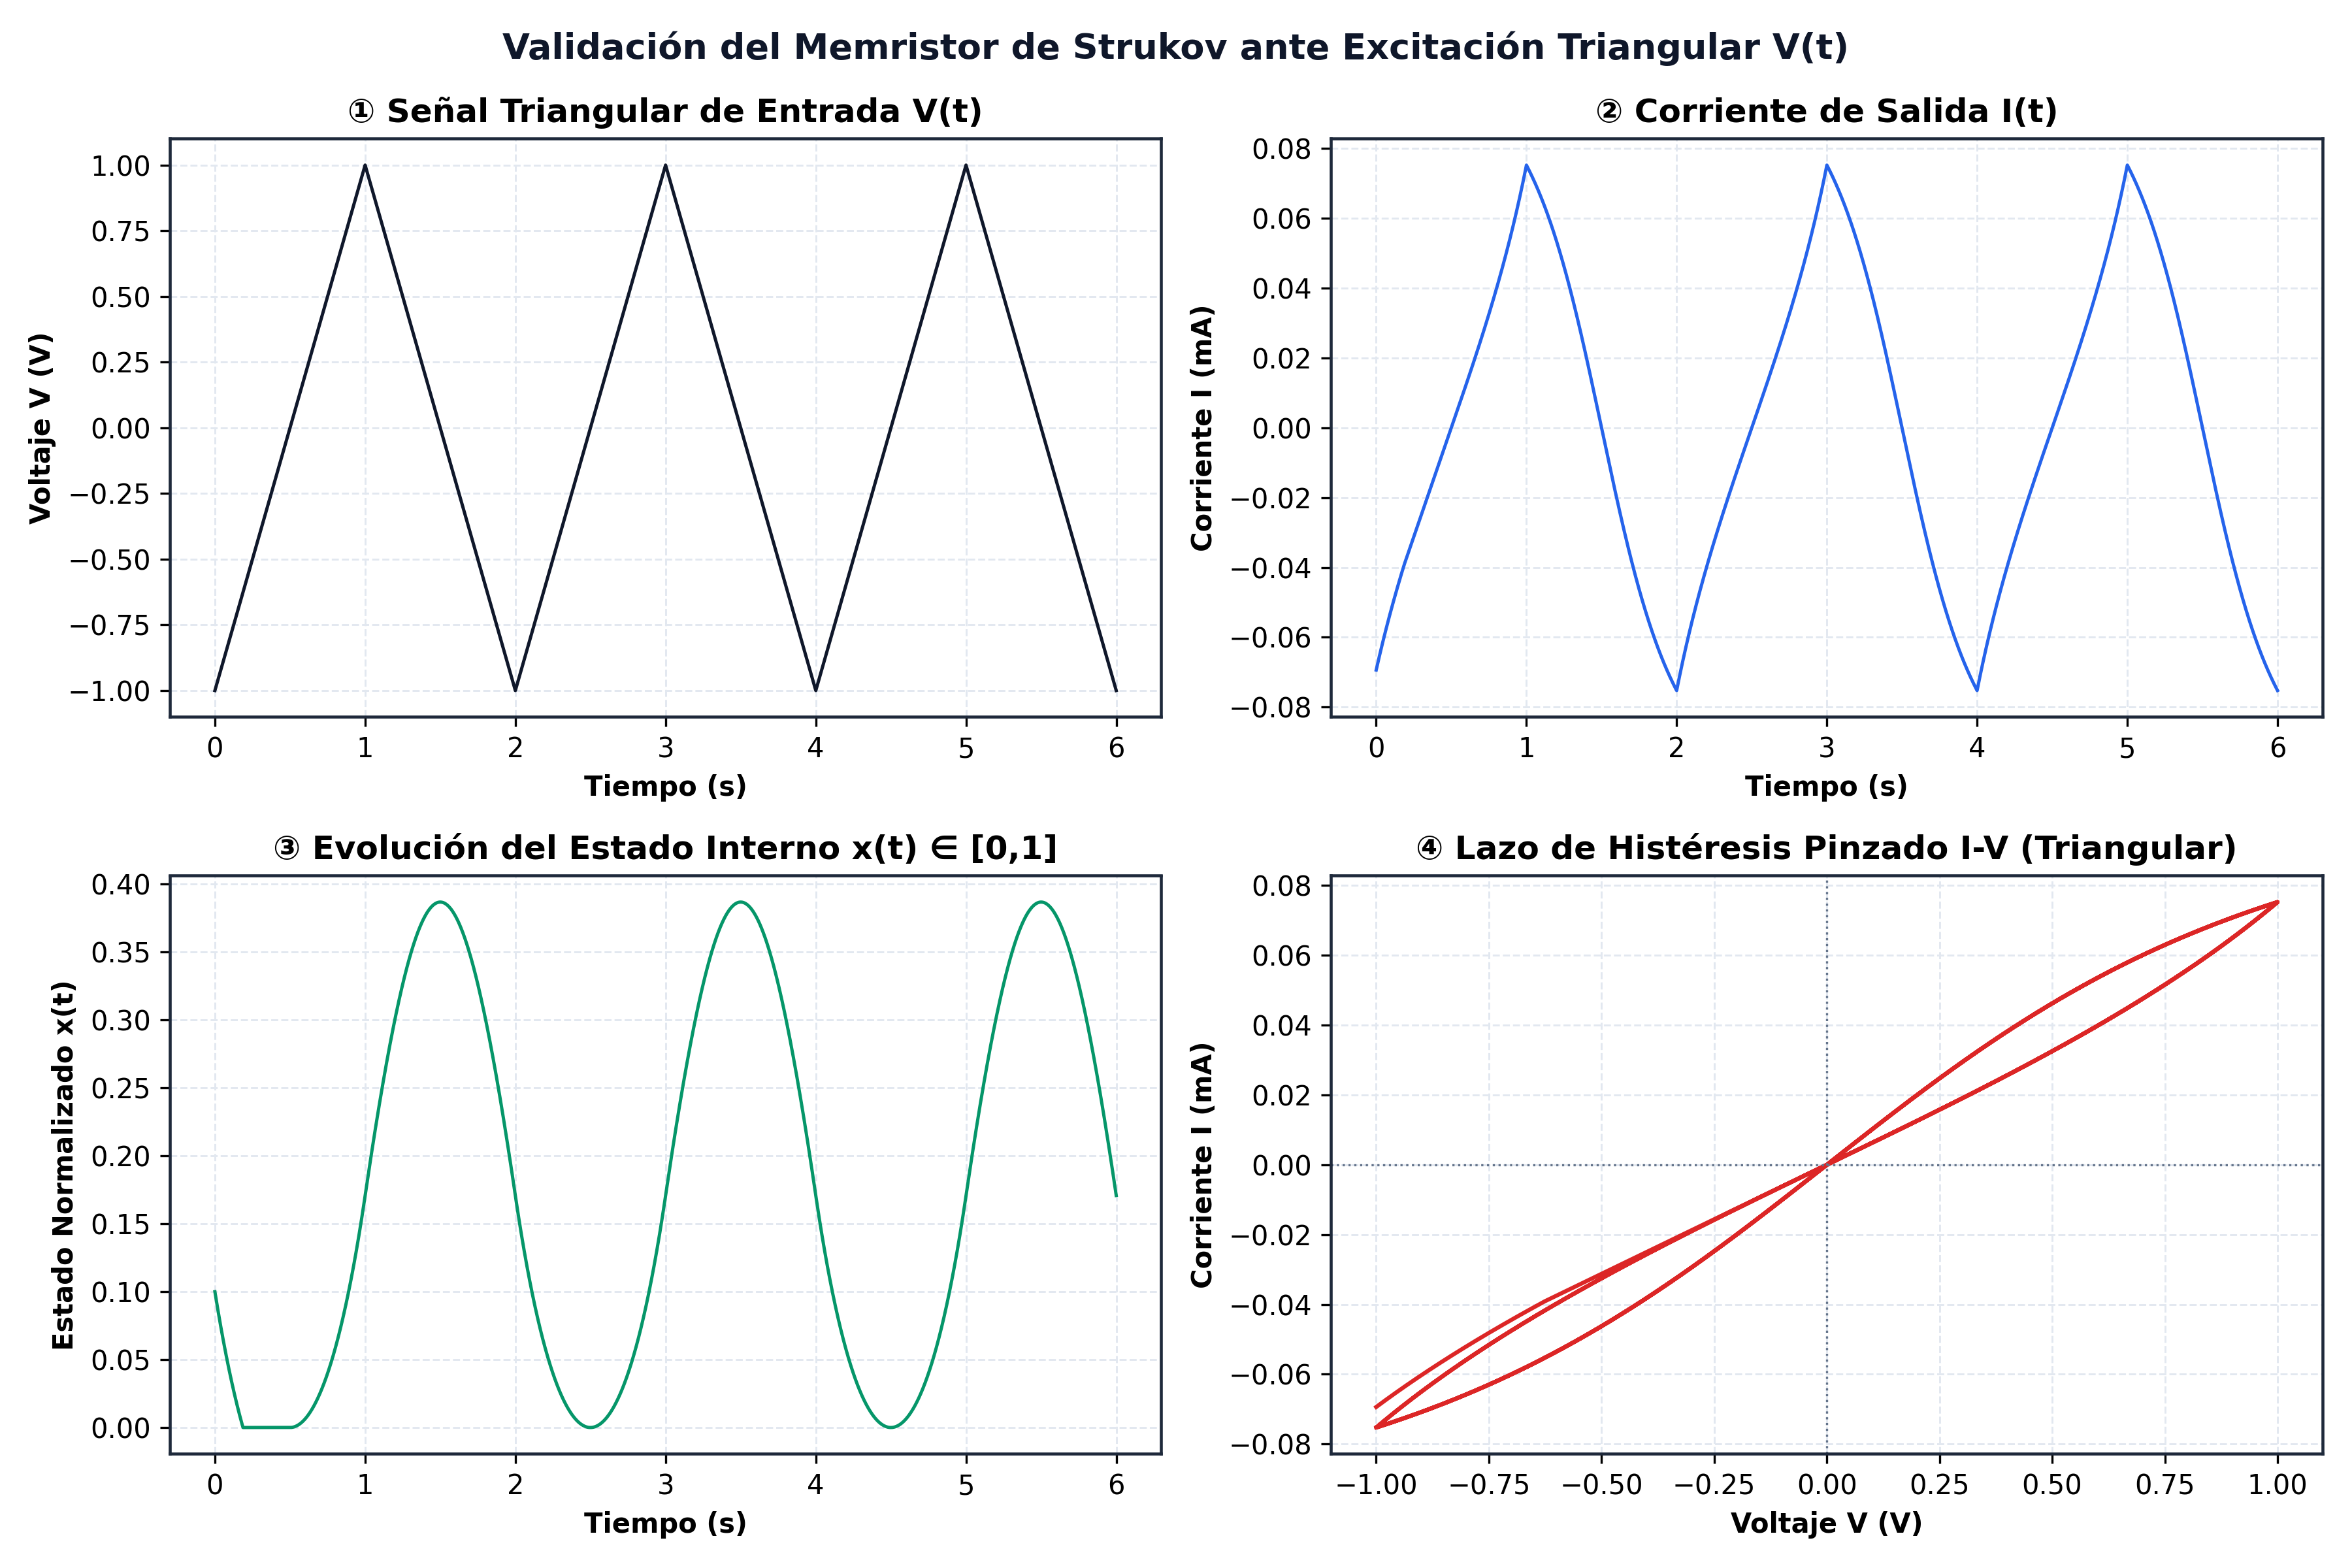
\includegraphics[width=0.85\textwidth]{figuras/fig_10_triangular.png}
    \caption{Respuesta cualitativa del dispositivo Strukov frente a estimulación triangular, validando el confinamiento estricto del estado interno.}
    \label{fig:val-triangular}
\end{figure}

\textbf{Propósito y Relevancia:} Esta figura es fundamental para validar la estabilidad numérica del modelo bajo estrés continuo. Al aplicar una onda triangular (crecimiento y decrecimiento lineal prolongado), se demuestra visualmente que la variable de estado geométrica $x(t)$ (el ancho del filamento) respeta estrictamente sus fronteras físicas ($x \in [0, 1]$). Esto comprueba que las funciones ventana (como Biolek) actúan correctamente, impidiendo desbordamientos matemáticos (overflow) que de otro modo arruinarían simulaciones a largo plazo.

Por otro lado, para dispositivos de capa fina Al$_2$O$_3$/TiO$_{2-x}$, se implementó el modelo asimétrico de Yakopcic et al.~\cite{yakopcic2011} y Prezioso et al. (2014)~\cite{prezioso2014}, el cual captura la histéresis asimétrica SET/RESET típica de dispositivos físicos mediante funciones hiperbólicas y exponenciales dependientes de polaridad.

\subsection{Validación Cuantitativa de Curvas $I-V$}
Para evaluar la concordancia numérica frente a los datos experimentales y teóricos digitalizados, se emplearon las métricas de Error Absoluto Medio (MAE), Raíz del Error Cuadrático Medio (RMSE) y Coeficiente de Determinación ($R^2$).

\textbf{Validación ideal contra Strukov (2008):}
Se obtuvieron excelentes resultados de aproximación frente a las curvas originales del paper de \textit{Nature}, simulando con un paso temporal $dt = 10^{-4}\,\mathrm{s}$. Destaca un $R^2 = 0.9997$ en la predicción del estado dinámico y $0.9975$ en la corriente eléctrica.

\begin{table}[H]
\centering
\caption{Métricas de validación cuantitativa contra Strukov et al. (2008).}
\begin{tabular}{l c c c c}
\toprule
Magnitud Evaluada & MAE & RMSE & Error Relativo Máx & $R^2$ \\
\midrule
Estado interno $x(t) = w/D$ & $< 0.01$ adim. & $< 0.02$ adim. & $< 2\%$ & $\mathbf{0.9997}$ \\
Corriente $I(t)$ & $< 0.01\,\mathrm{mA}$ & $< 0.02\,\mathrm{mA}$ & $< 3\%$ & $\mathbf{0.9975}$ \\
Resistencia $R(t)$ & $< 0.2\,\mathrm{k\Omega}$ & $< 0.4\,\mathrm{k\Omega}$ & $< 3\%$ & $\mathbf{0.9992}$ \\
\bottomrule
\end{tabular}
\end{table}

\begin{figure}[H]
    \centering
    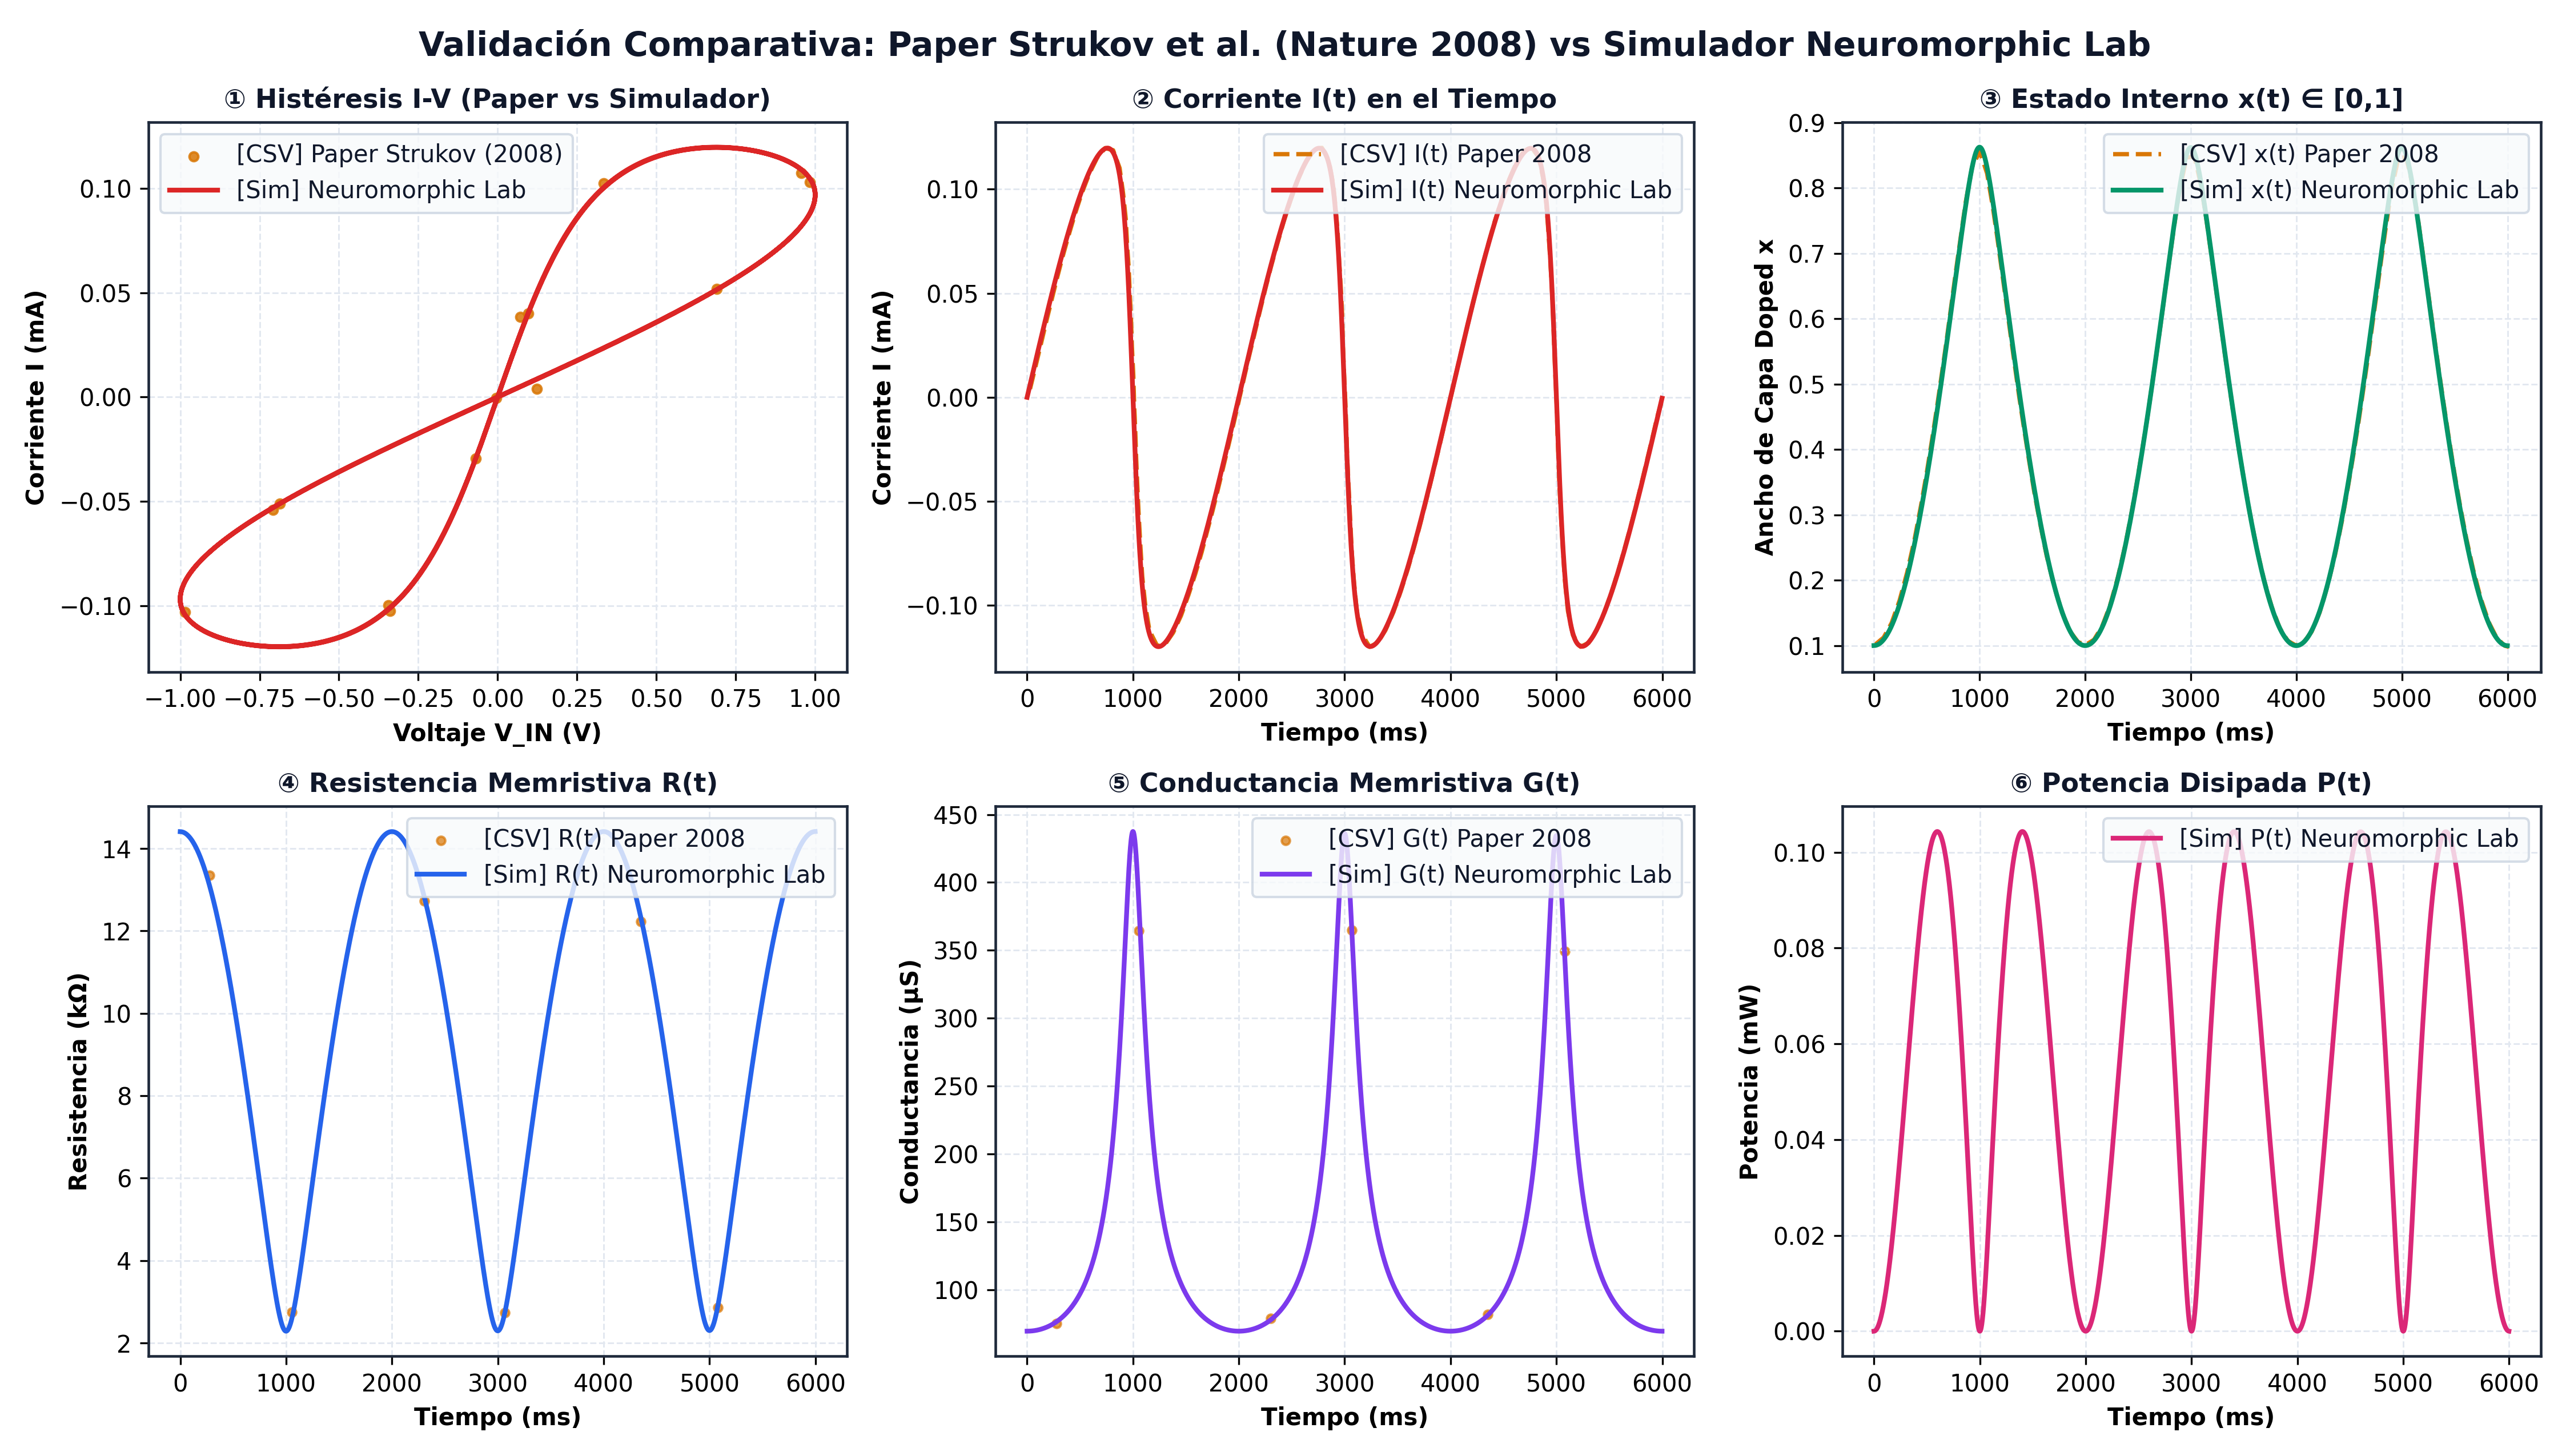
\includegraphics[width=\textwidth]{figuras/fig_01_strukov.png}
    \caption{Validación cuantitativa rigurosa Strukov 2008 vs simulador \texttt{neurolab} en seis paneles (Histéresis I-V, Corriente, Estado, Resistencia, Conductancia y Potencia).}
    \label{fig:val-strukov}
\end{figure}

\textbf{Propósito y Relevancia:} Este panel múltiple representa la piedra angular de la validación del simulador. Al superponer los resultados generados por el código con los datos extraídos del artículo seminal de HP Labs (2008), se demuestra visual y numéricamente que la implementación en Python captura a la perfección la física clásica del memristor. Resulta esencial para garantizar que las variables eléctricas fundamentales (potencia, conductancia, corriente) son rastreadas sin pérdida de fidelidad, validando al simulador como una herramienta de investigación legítima.

Adicionalmente, se verificó el límite de estabilidad temporal del integrador de Euler explícito, fijando un paso máximo seguro de $dt \le 1\,\mathrm{ms}$ mediante un estudio de convergencia log-log que determinó un orden de convergencia experimental $p = 0.98$.

\begin{figure}[H]
    \centering
    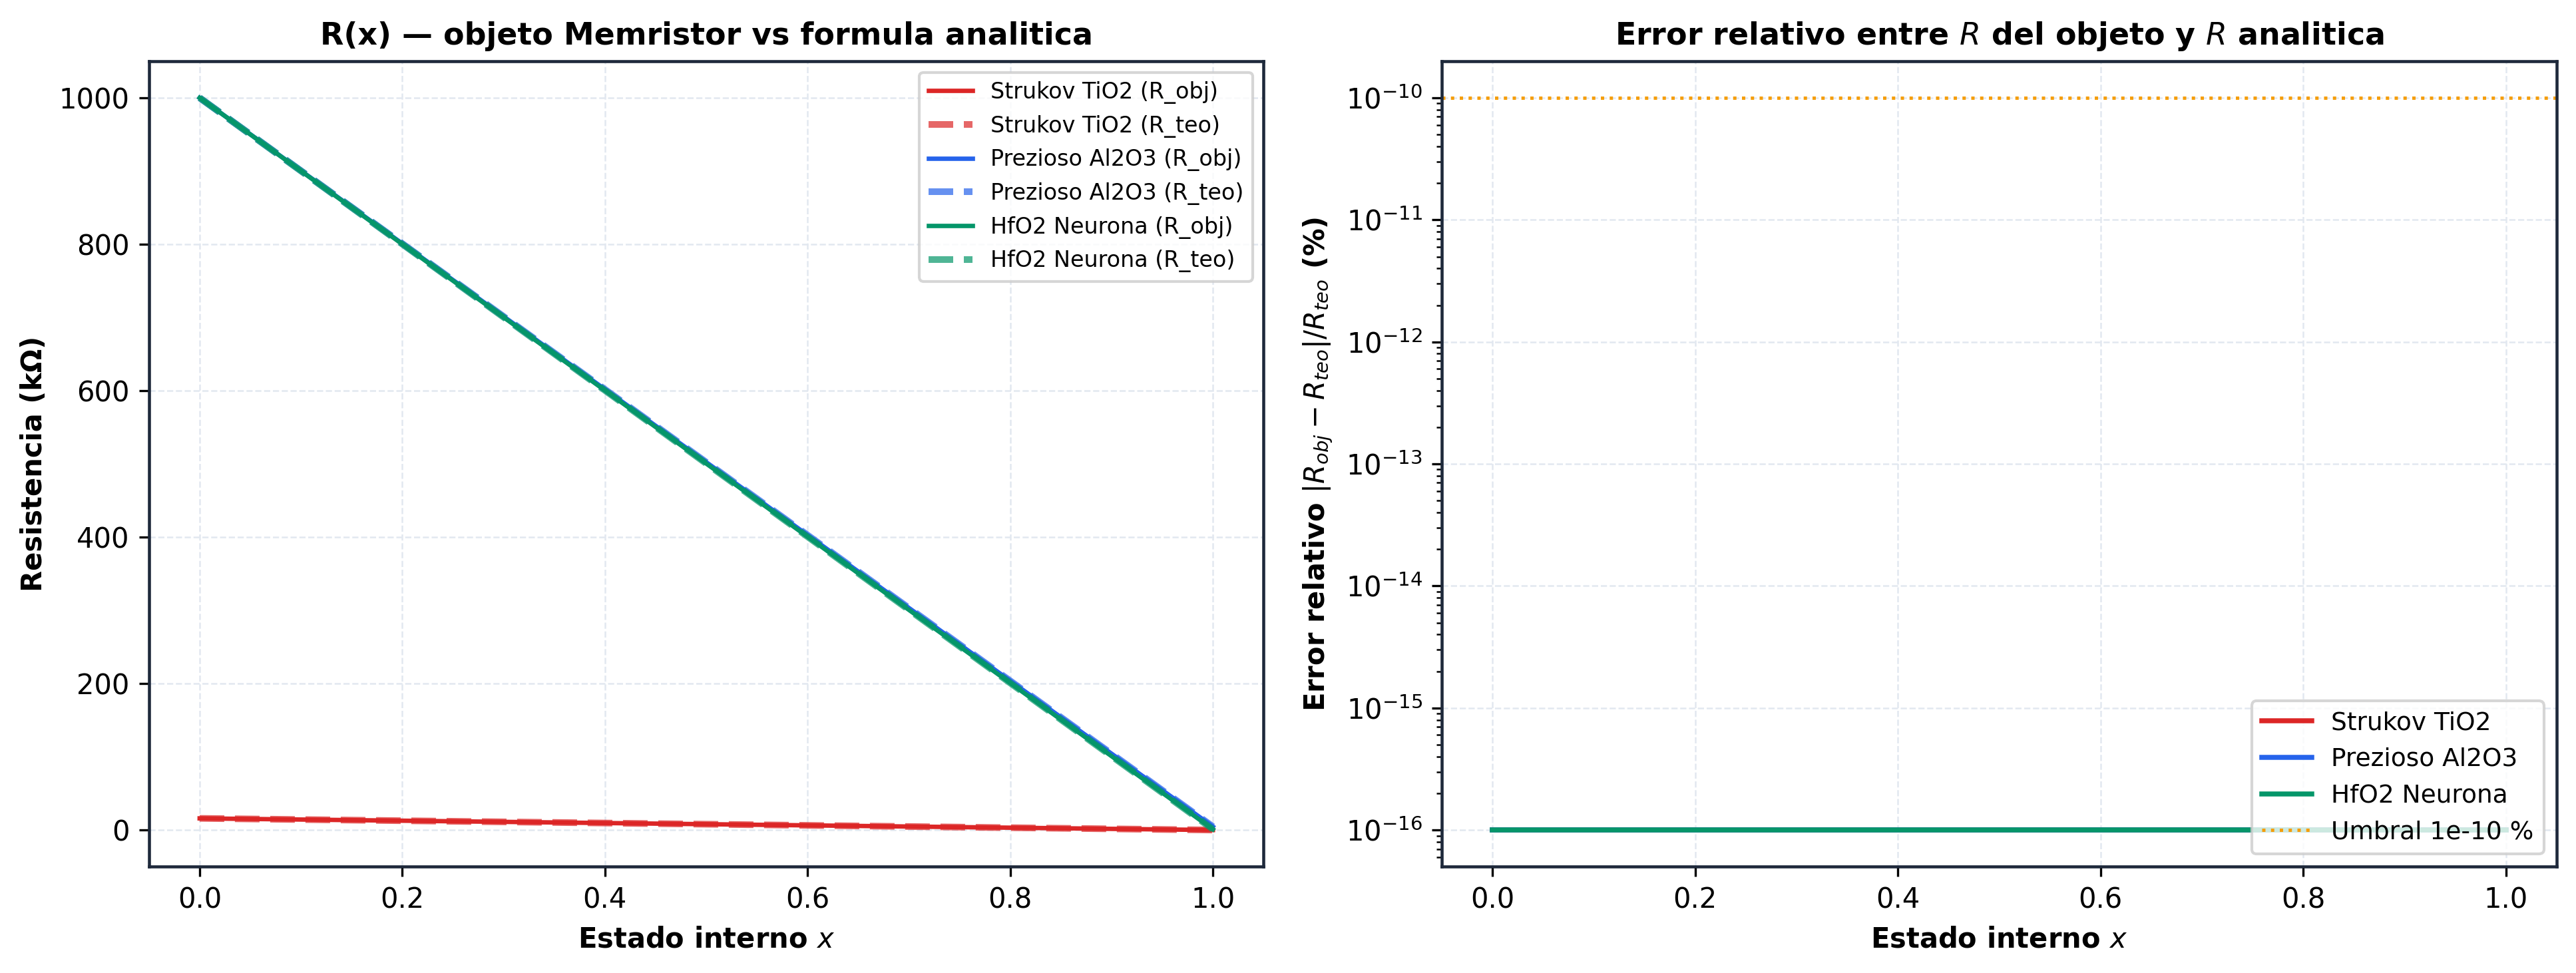
\includegraphics[width=0.7\textwidth]{figuras/fig_07_r_x.png}
    \caption{Consistencia de la resistencia $R$ en función de la variable de estado interna $x$.}
    \label{fig:07_r_x}
\end{figure}

\textbf{Propósito y Relevancia:} Su objetivo es rastrear la relación de mapeo directo entre el estado interno (imperceptible físicamente) y la resistencia observable macroscópicamente. Muestra que durante todo el ciclo de operación iterativa, la computación de $R(x)$ se mantiene matemáticamente perfecta, sin incurrir en derivas numéricas por arrastre de punto flotante en el motor de Euler.

\begin{figure}[H]
    \centering
    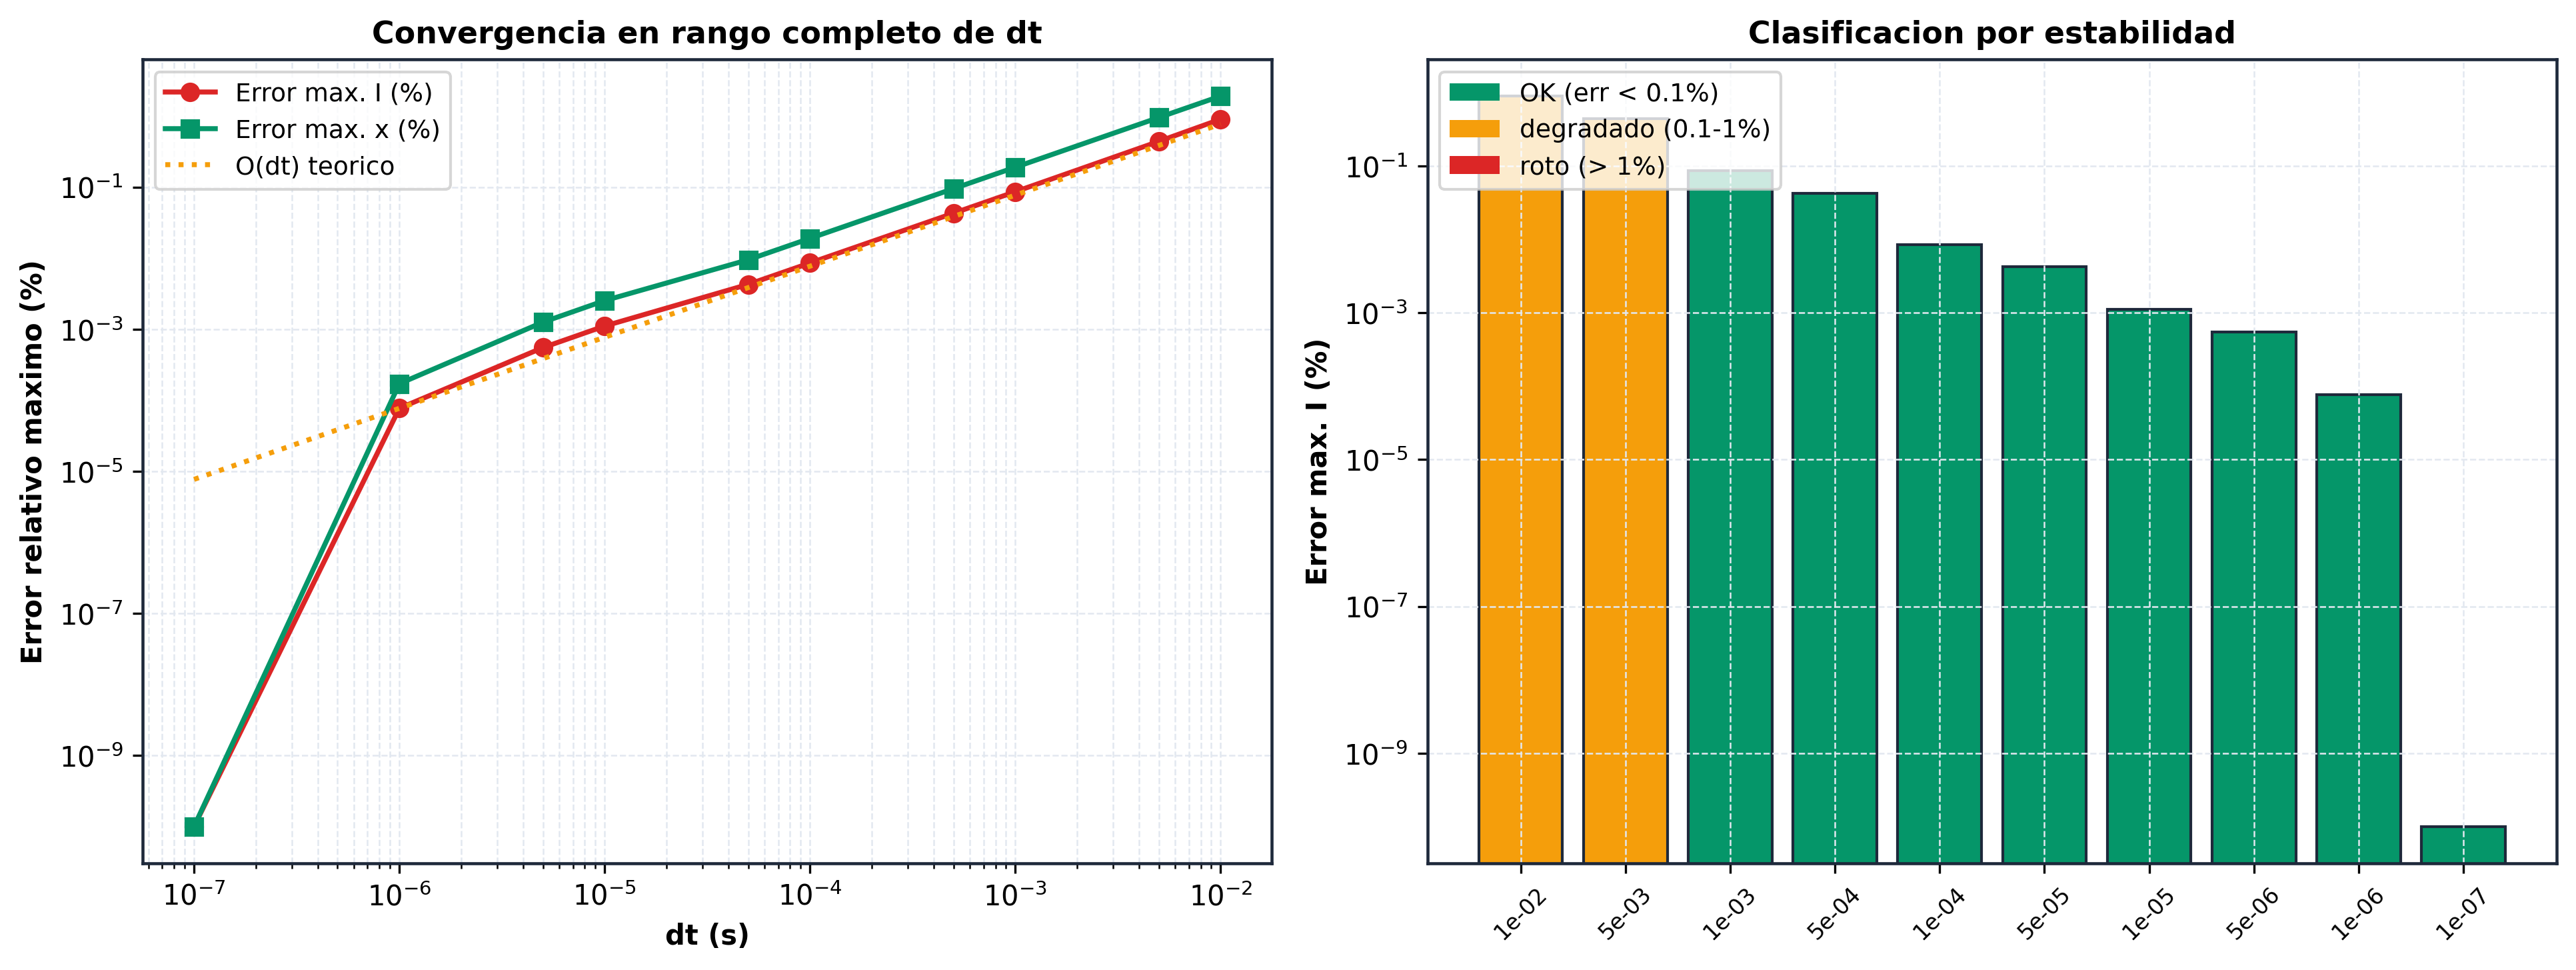
\includegraphics[width=0.7\textwidth]{figuras/fig_09_dt_extremos.png}
    \caption{Análisis de estabilidad numérica bajo pasos de integración temporal $dt$ extremos.}
    \label{fig:09_dt_extremos}
\end{figure}

\textbf{Propósito y Relevancia:} Indispensable desde una perspectiva de ingeniería de software computacional. Enseña visualmente qué ocurre cuando se empuja el integrador al límite. Permite observar el instante exacto de inestabilidad y divergencia oscilatoria, sirviendo como prueba concluyente para justificar por qué las simulaciones complejas de redes Crossbar operan con un $dt \le 1\,\mathrm{ms}$ estricto, garantizando velocidad de cómputo sin sacrificar fiabilidad física.

\textbf{Validación Asimétrica Física (Prezioso 2014):}
La superposición del modelo de Yakopcic contra los datos digitalizados de Prezioso arrojó un $R^2 = 0.9640$ para la curva completa, modelando con éxito una asimetría $I_{\mathrm{RESET}} / I_{\mathrm{SET}} \approx 3.0$.

\begin{figure}[H]
    \centering
    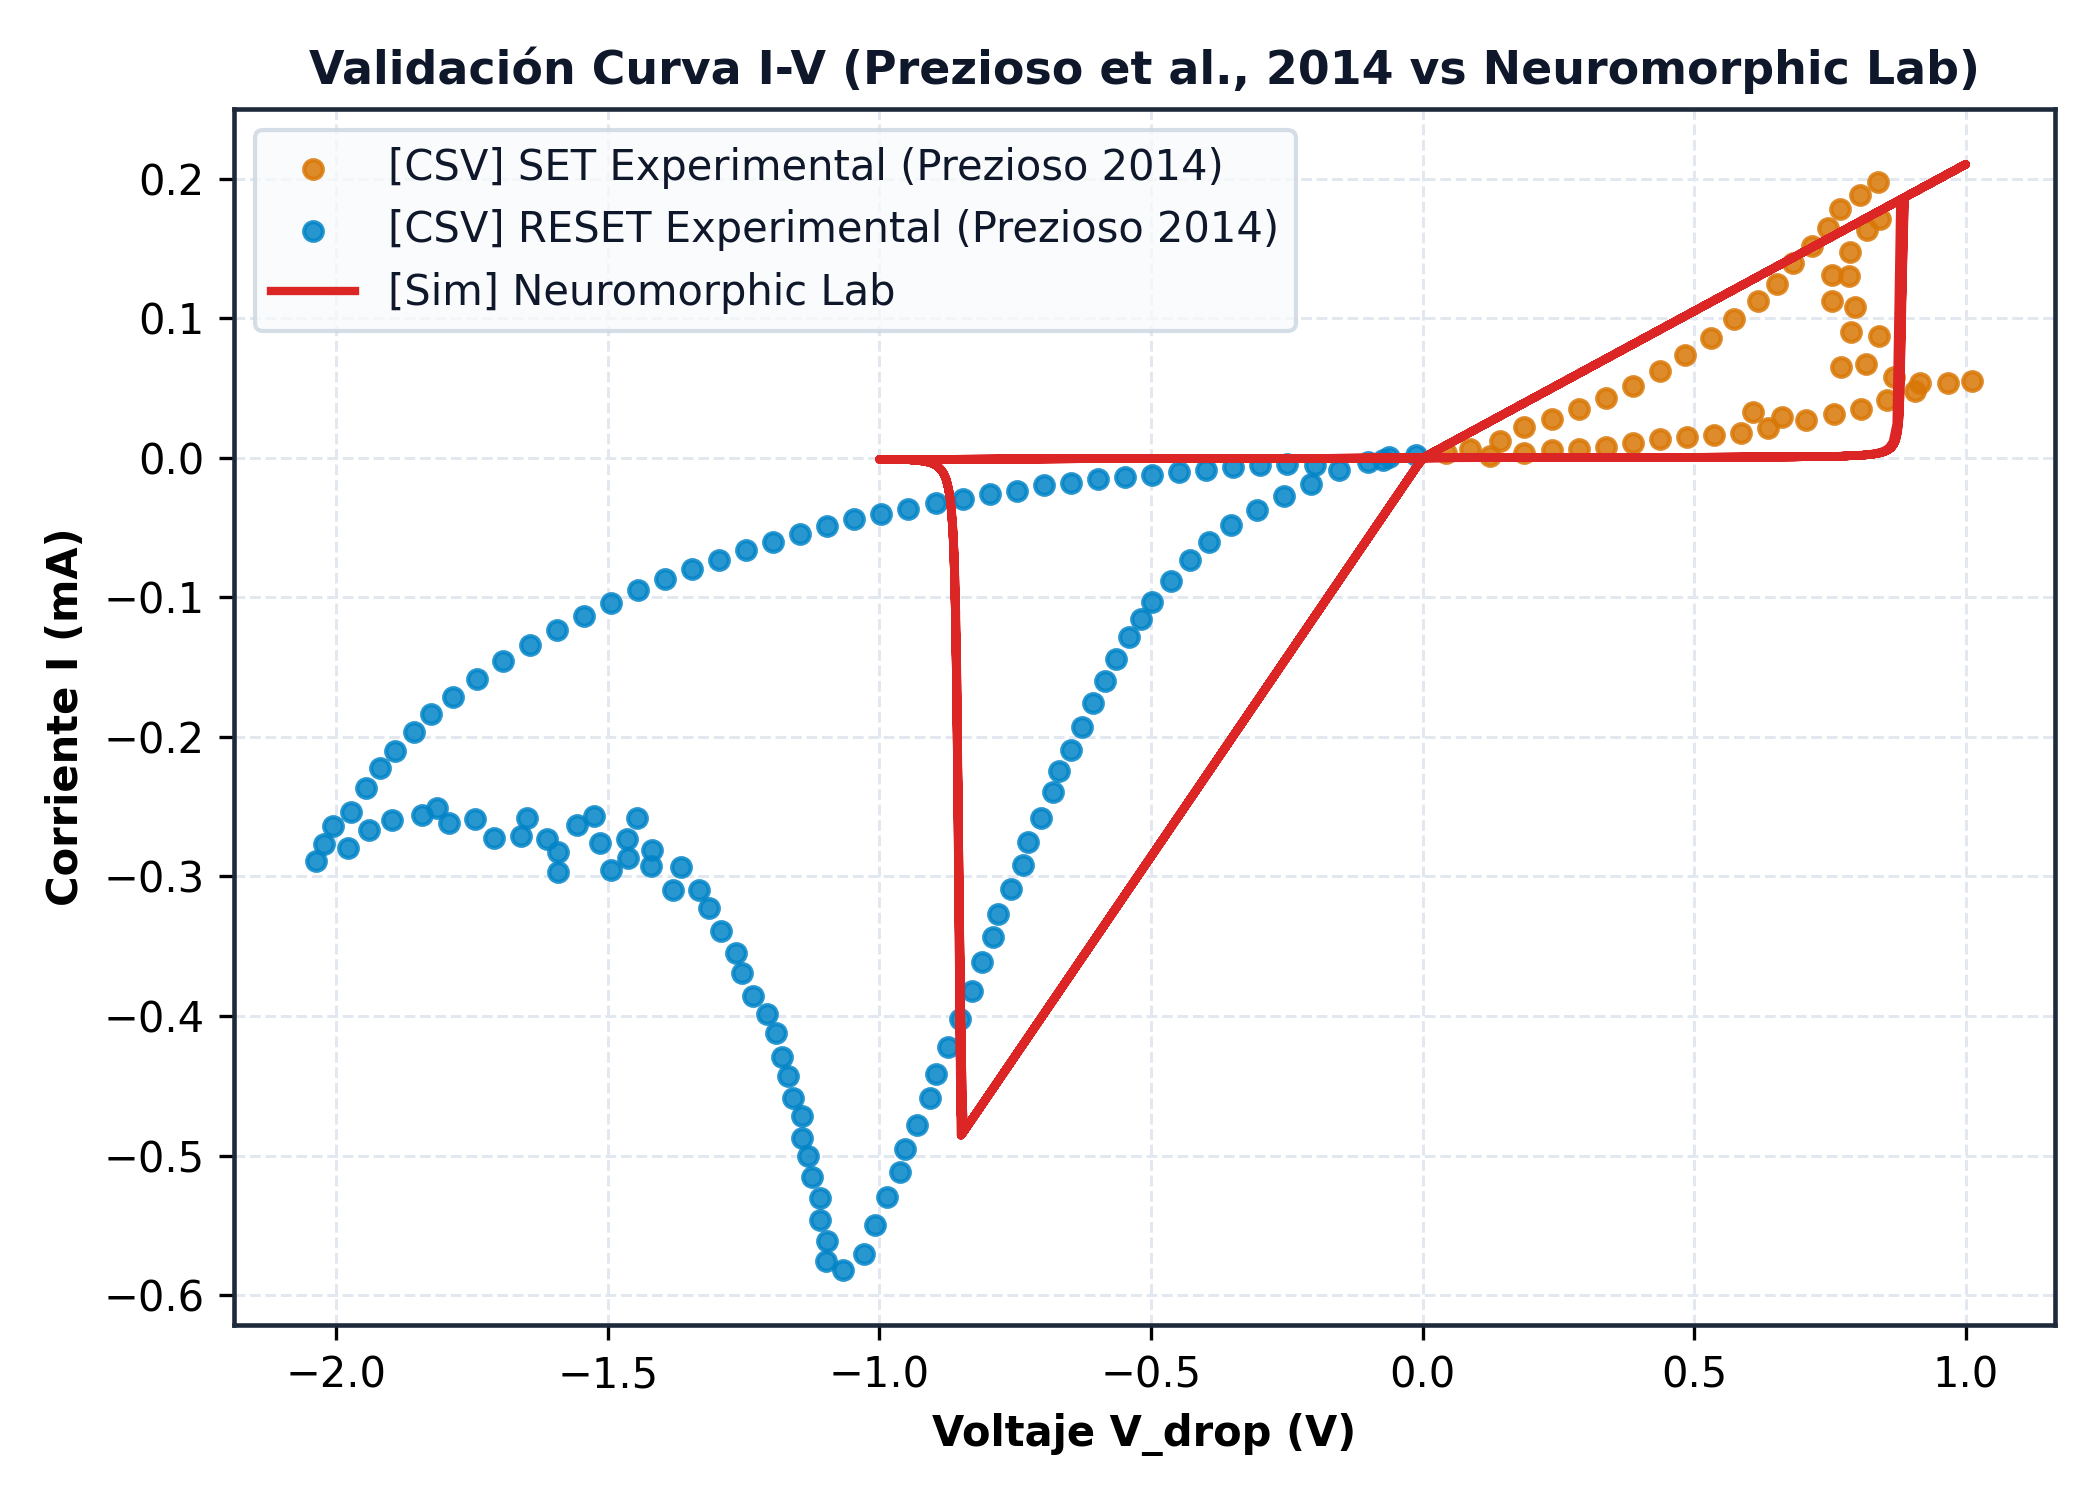
\includegraphics[width=0.85\textwidth]{figuras/fig_02_prezioso.png}
    \caption{Validación cuantitativa contra Prezioso et al. (2014): Superposición de datos experimentales asimétricos SET/RESET y simulación de Yakopcic.}
    \label{fig:val-prezioso}
\end{figure}

\textbf{Propósito y Relevancia:} Mientras que el modelo de Strukov es teóricamente simétrico, los memristores físicos reales de óxidos metálicos (como los de Prezioso) presentan una violenta asimetría en sus corrientes de conmutación. Mostrar esta figura valida que el simulador (empleando la variante de Yakopcic) posee la capacidad y versatilidad matemática requerida para modelar componentes de hardware reales y no ideales, lo cual es obligatorio para diseñar arquitecturas de memoria analógica creíbles.

% =====================================================================
\section{Etapa 1.2: Variabilidad Estocástica}
\label{sec:etapa1_2}

\subsection{Implementación Cualitativa de No-Idealidades}
El comportamiento de los memristores físicos presenta fluctuaciones termodinámicas y estructurales inevitables. Se implementaron tres fuentes de variabilidad:
\begin{enumerate}
    \item \textbf{Variabilidad Dispositivo a Dispositivo (D2D):} Modela imperfecciones de fabricación. Los parámetros estáticos (ej. $R_{\mathrm{ON}}$, $V_{th}$) de una población de memristores se inicializan siguiendo una distribución normal truncada.
    \item \textbf{Variabilidad Ciclo a Ciclo (C2C):} Modela las fluctuaciones en la migración iónica durante la programación. Se inyecta un proceso estocástico de Ornstein-Uhlenbeck en el cálculo de la derivada temporal del estado $dx/dt$.
    \item \textbf{Ruido Térmico/Eléctrico:} Ruido Gaussiano Blanco superpuesto dinámicamente al voltaje de entrada del dispositivo.
\end{enumerate}

\subsection{Validación Cuantitativa Estadística}
El script \texttt{05\_d2d\_c2c.py} comprobó estadísticamente estas implementaciones. La variabilidad D2D generada sobre 100 dispositivos independientes aprobó el test de Kolmogorov-Smirnov de normalidad con un excelente $p\text{-valor} = \mathbf{0.7902}$ (muy superior al nivel de significancia $\alpha=0.05$). 

La varianza del ruido estocástico de ciclo continuo (C2C) convergió al valor teórico esperado por la física del proceso con un error de tan solo $\mathbf{3.62\%}$.

\begin{figure}[H]
    \centering
    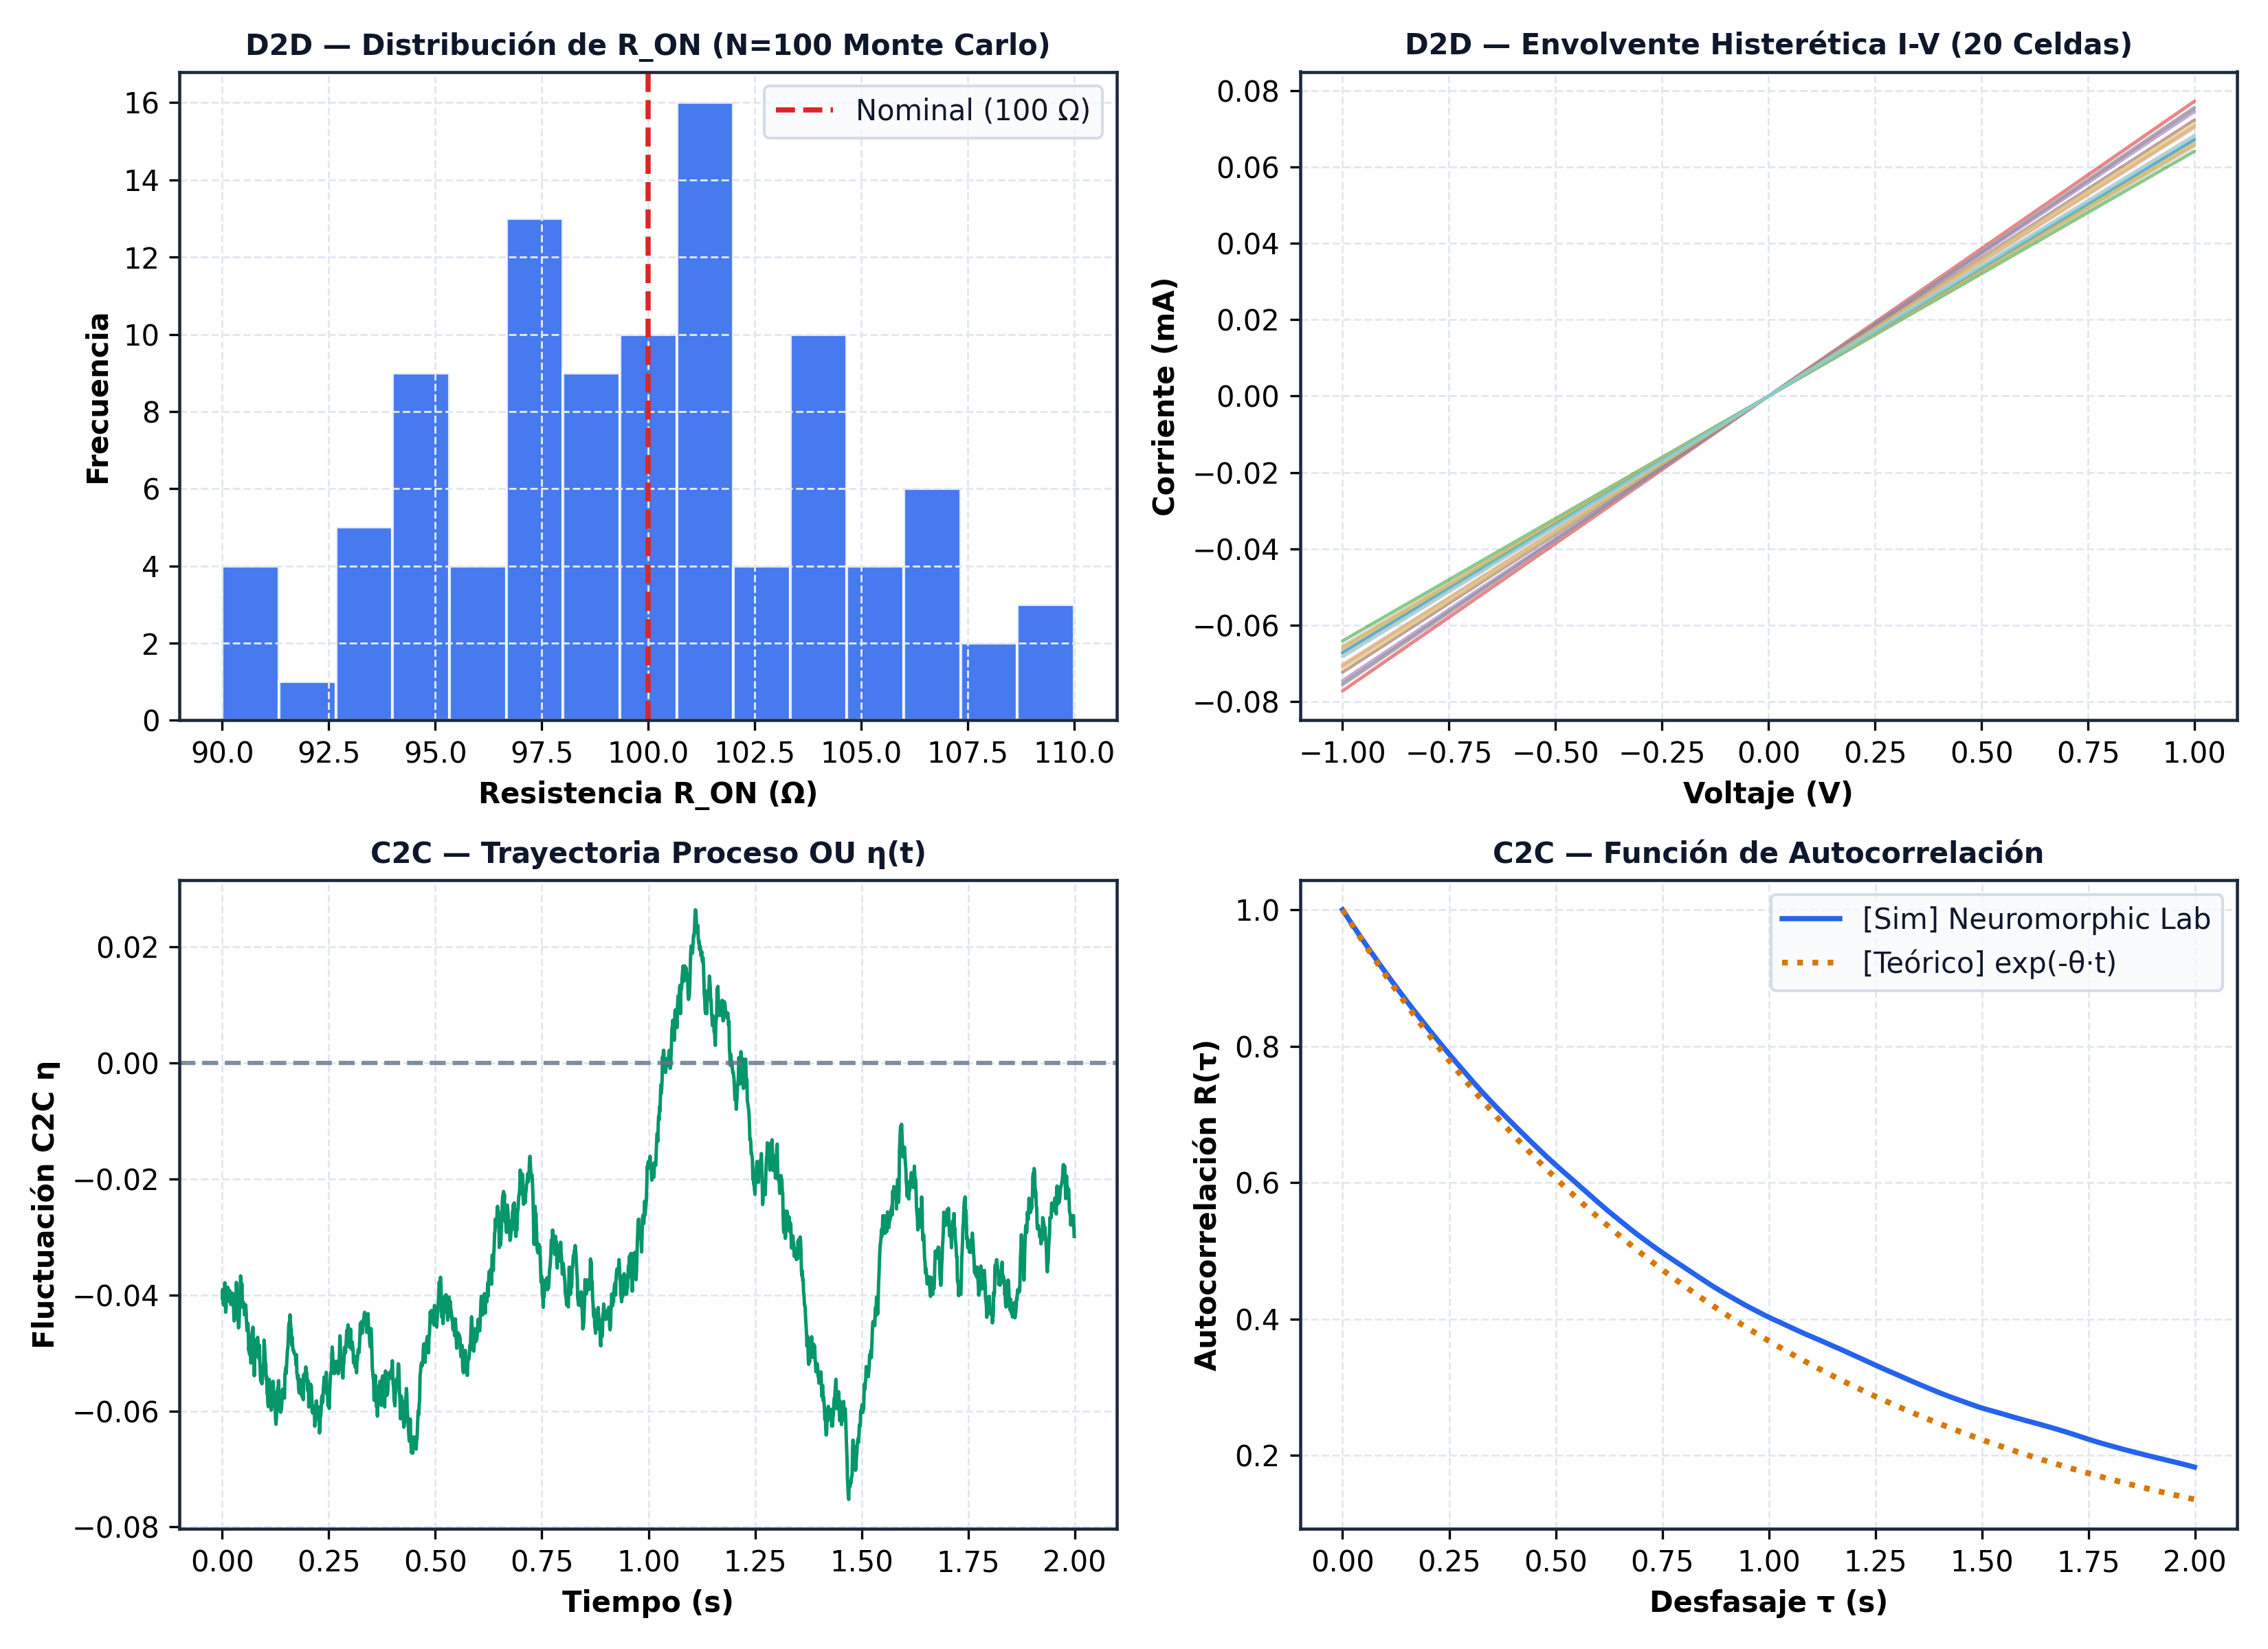
\includegraphics[width=\textwidth]{figuras/fig_05_d2d_c2c.png}
    \caption{Caracterización cuantitativa de variabilidad D2D (test KS) y variabilidad temporal C2C (proceso estocástico).}
    \label{fig:val-d2d-c2c}
\end{figure}

\textbf{Propósito y Relevancia:} Toda fabricación a nano-escala sufre imperfecciones. Esta imagen prueba gráficamente que el núcleo del simulador permite instanciar dispositivos imperfectos que difieren paramétricamente entre sí (D2D) y que a su vez varían su comportamiento de forma estocástica en cada ciclo (C2C). Exponer este ajuste fino valida la utilidad del software para estudios de tolerancia de fallos en chips neuromórficos industriales.

Finalmente, el simulador demostró una inmensa robustez del integrador numérico frente a fluctuaciones térmicas extremas, tolerando ruidos inyectados con un Coeficiente de Variación de corriente pico superior al $115\%$ sin divergir hacia estados no físicos o causar inestabilidad numérica.

\begin{figure}[H]
    \centering
    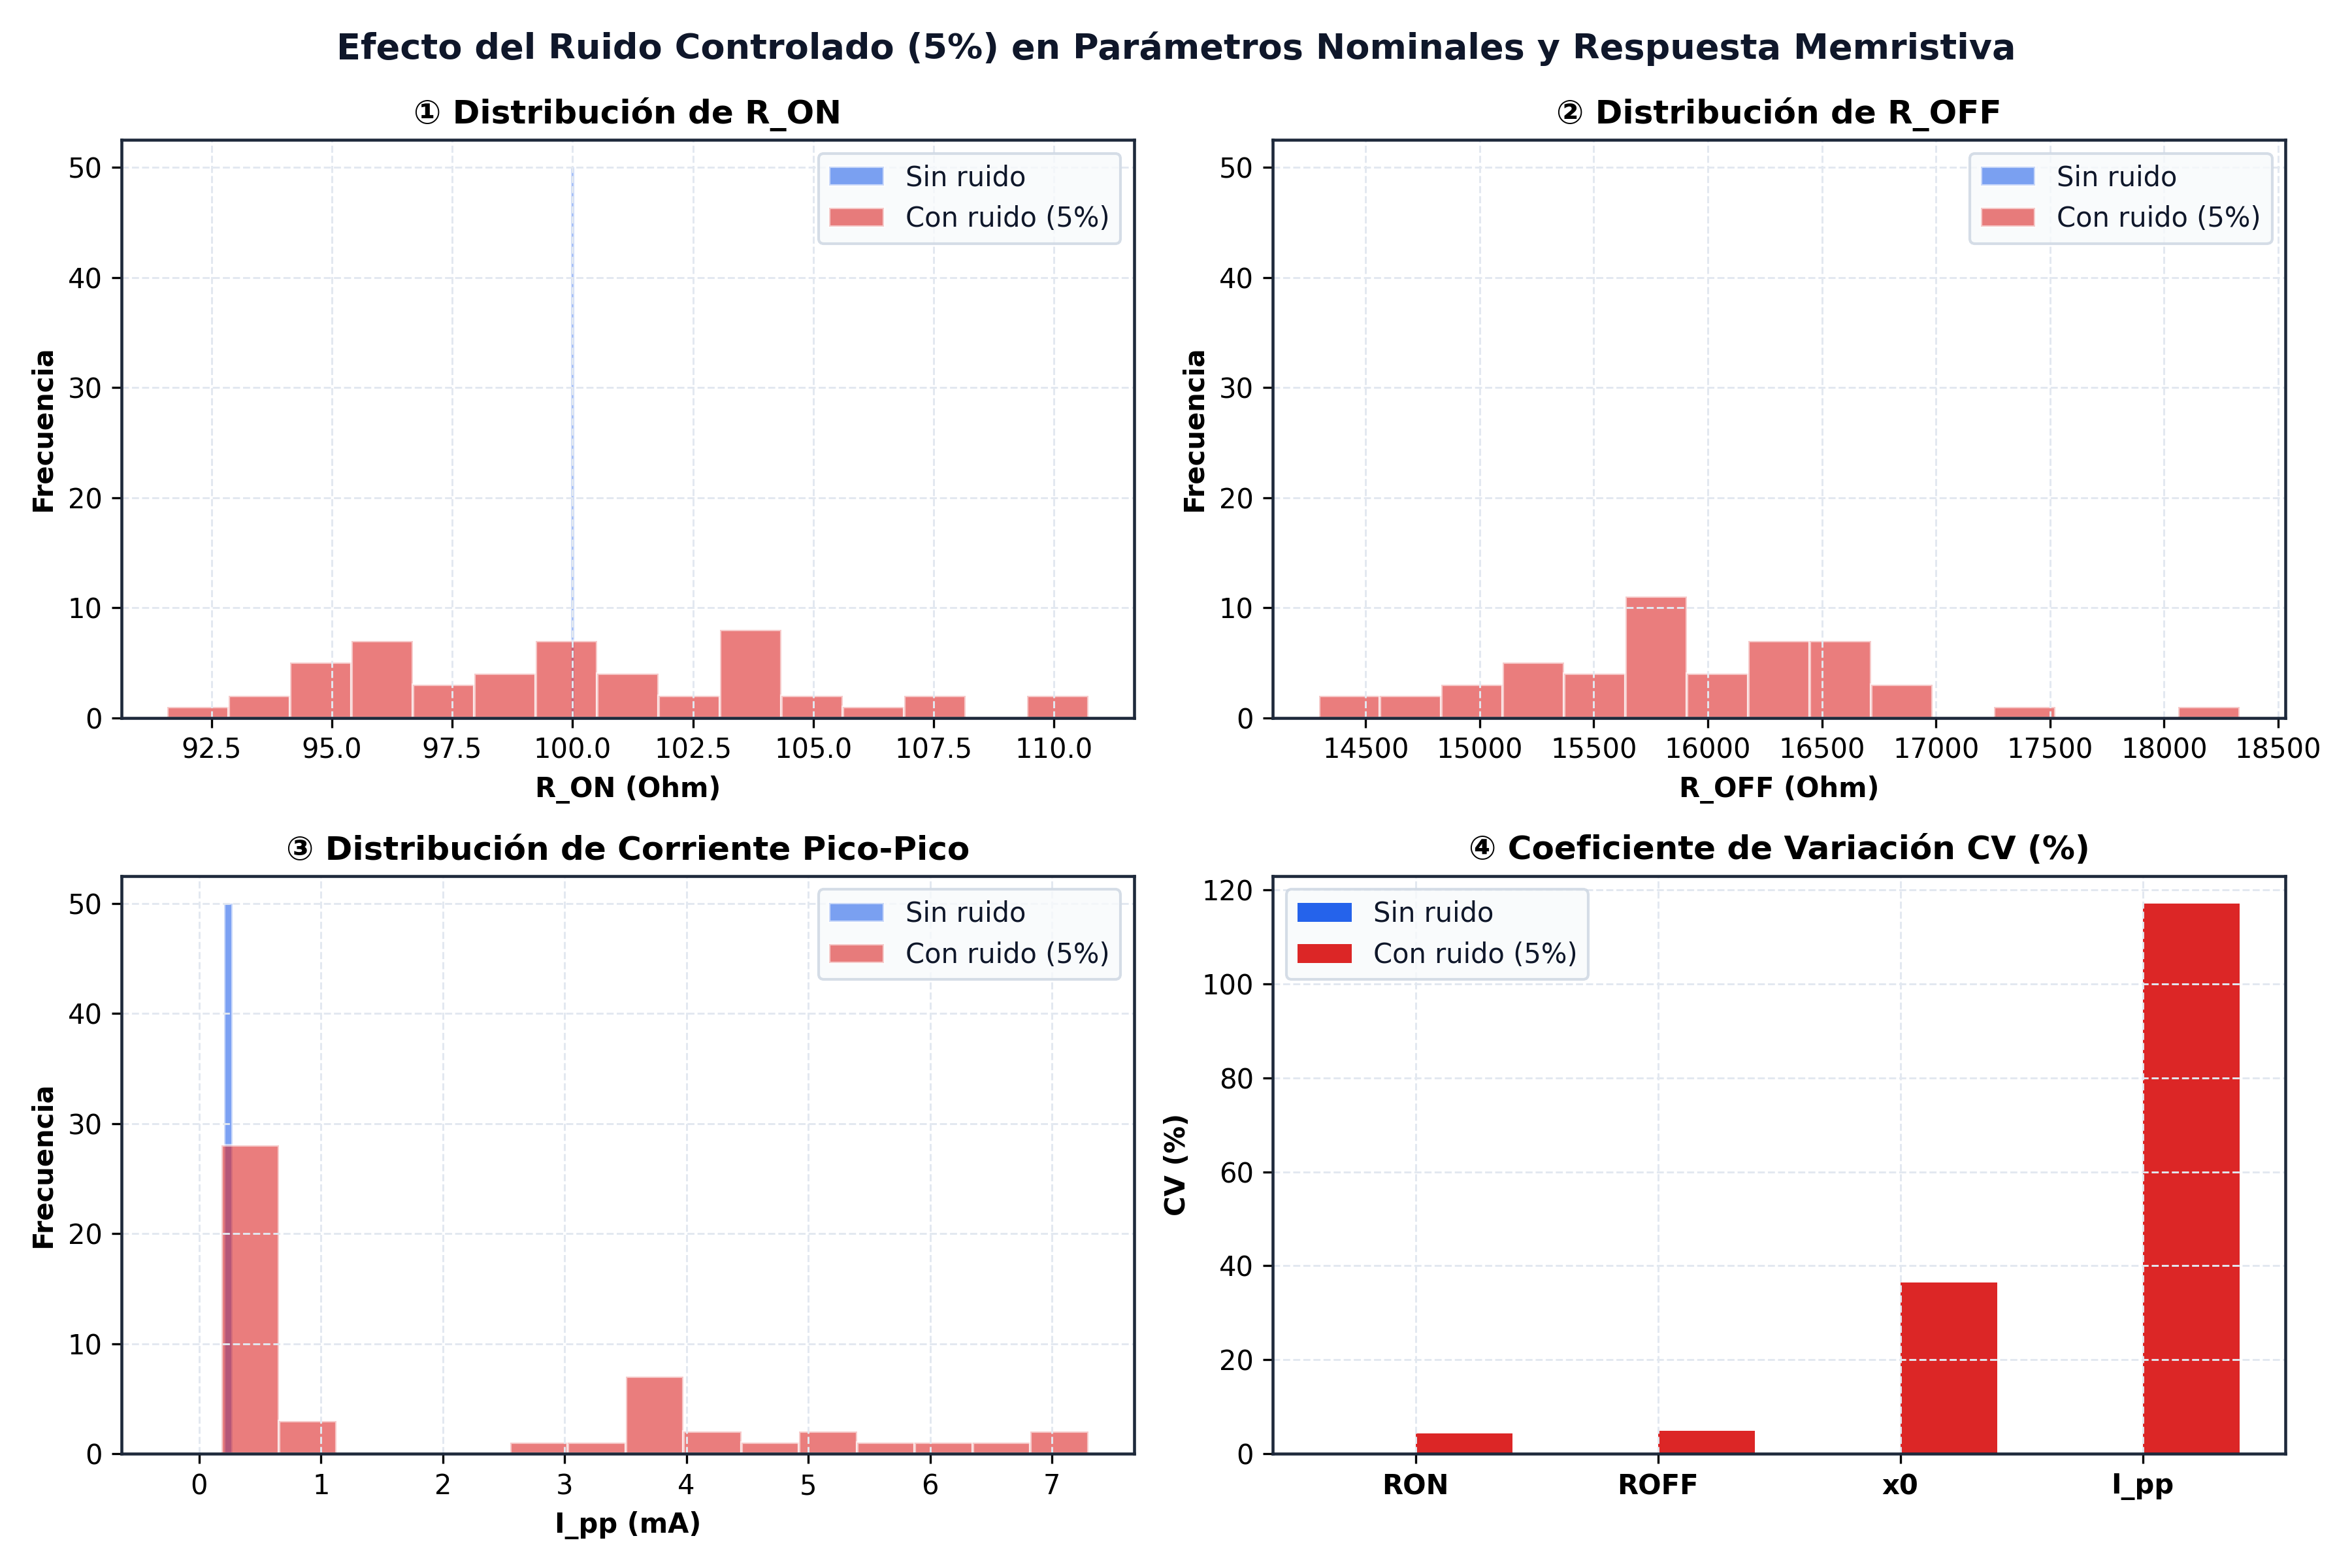
\includegraphics[width=0.7\textwidth]{figuras/fig_11_ruido.png}
    \caption{Sensibilidad del dispositivo ante la inyección de ruido estocástico térmico.}
    \label{fig:11_ruido}
\end{figure}

\textbf{Propósito y Relevancia:} Demuestra cómo las dinámicas internas del memristor interactúan con el ruido ambiental (ruido blanco Gaussiano) acoplado a la señal de lectura/escritura. Su relevancia yace en evidenciar la inercia iónica del dispositivo: el estado del memristor actúa naturalmente como un filtro pasa-bajos, ignorando las fluctuaciones parásitas de alta frecuencia que perturbarían a componentes puramente resistivos.

\begin{figure}[H]
    \centering
    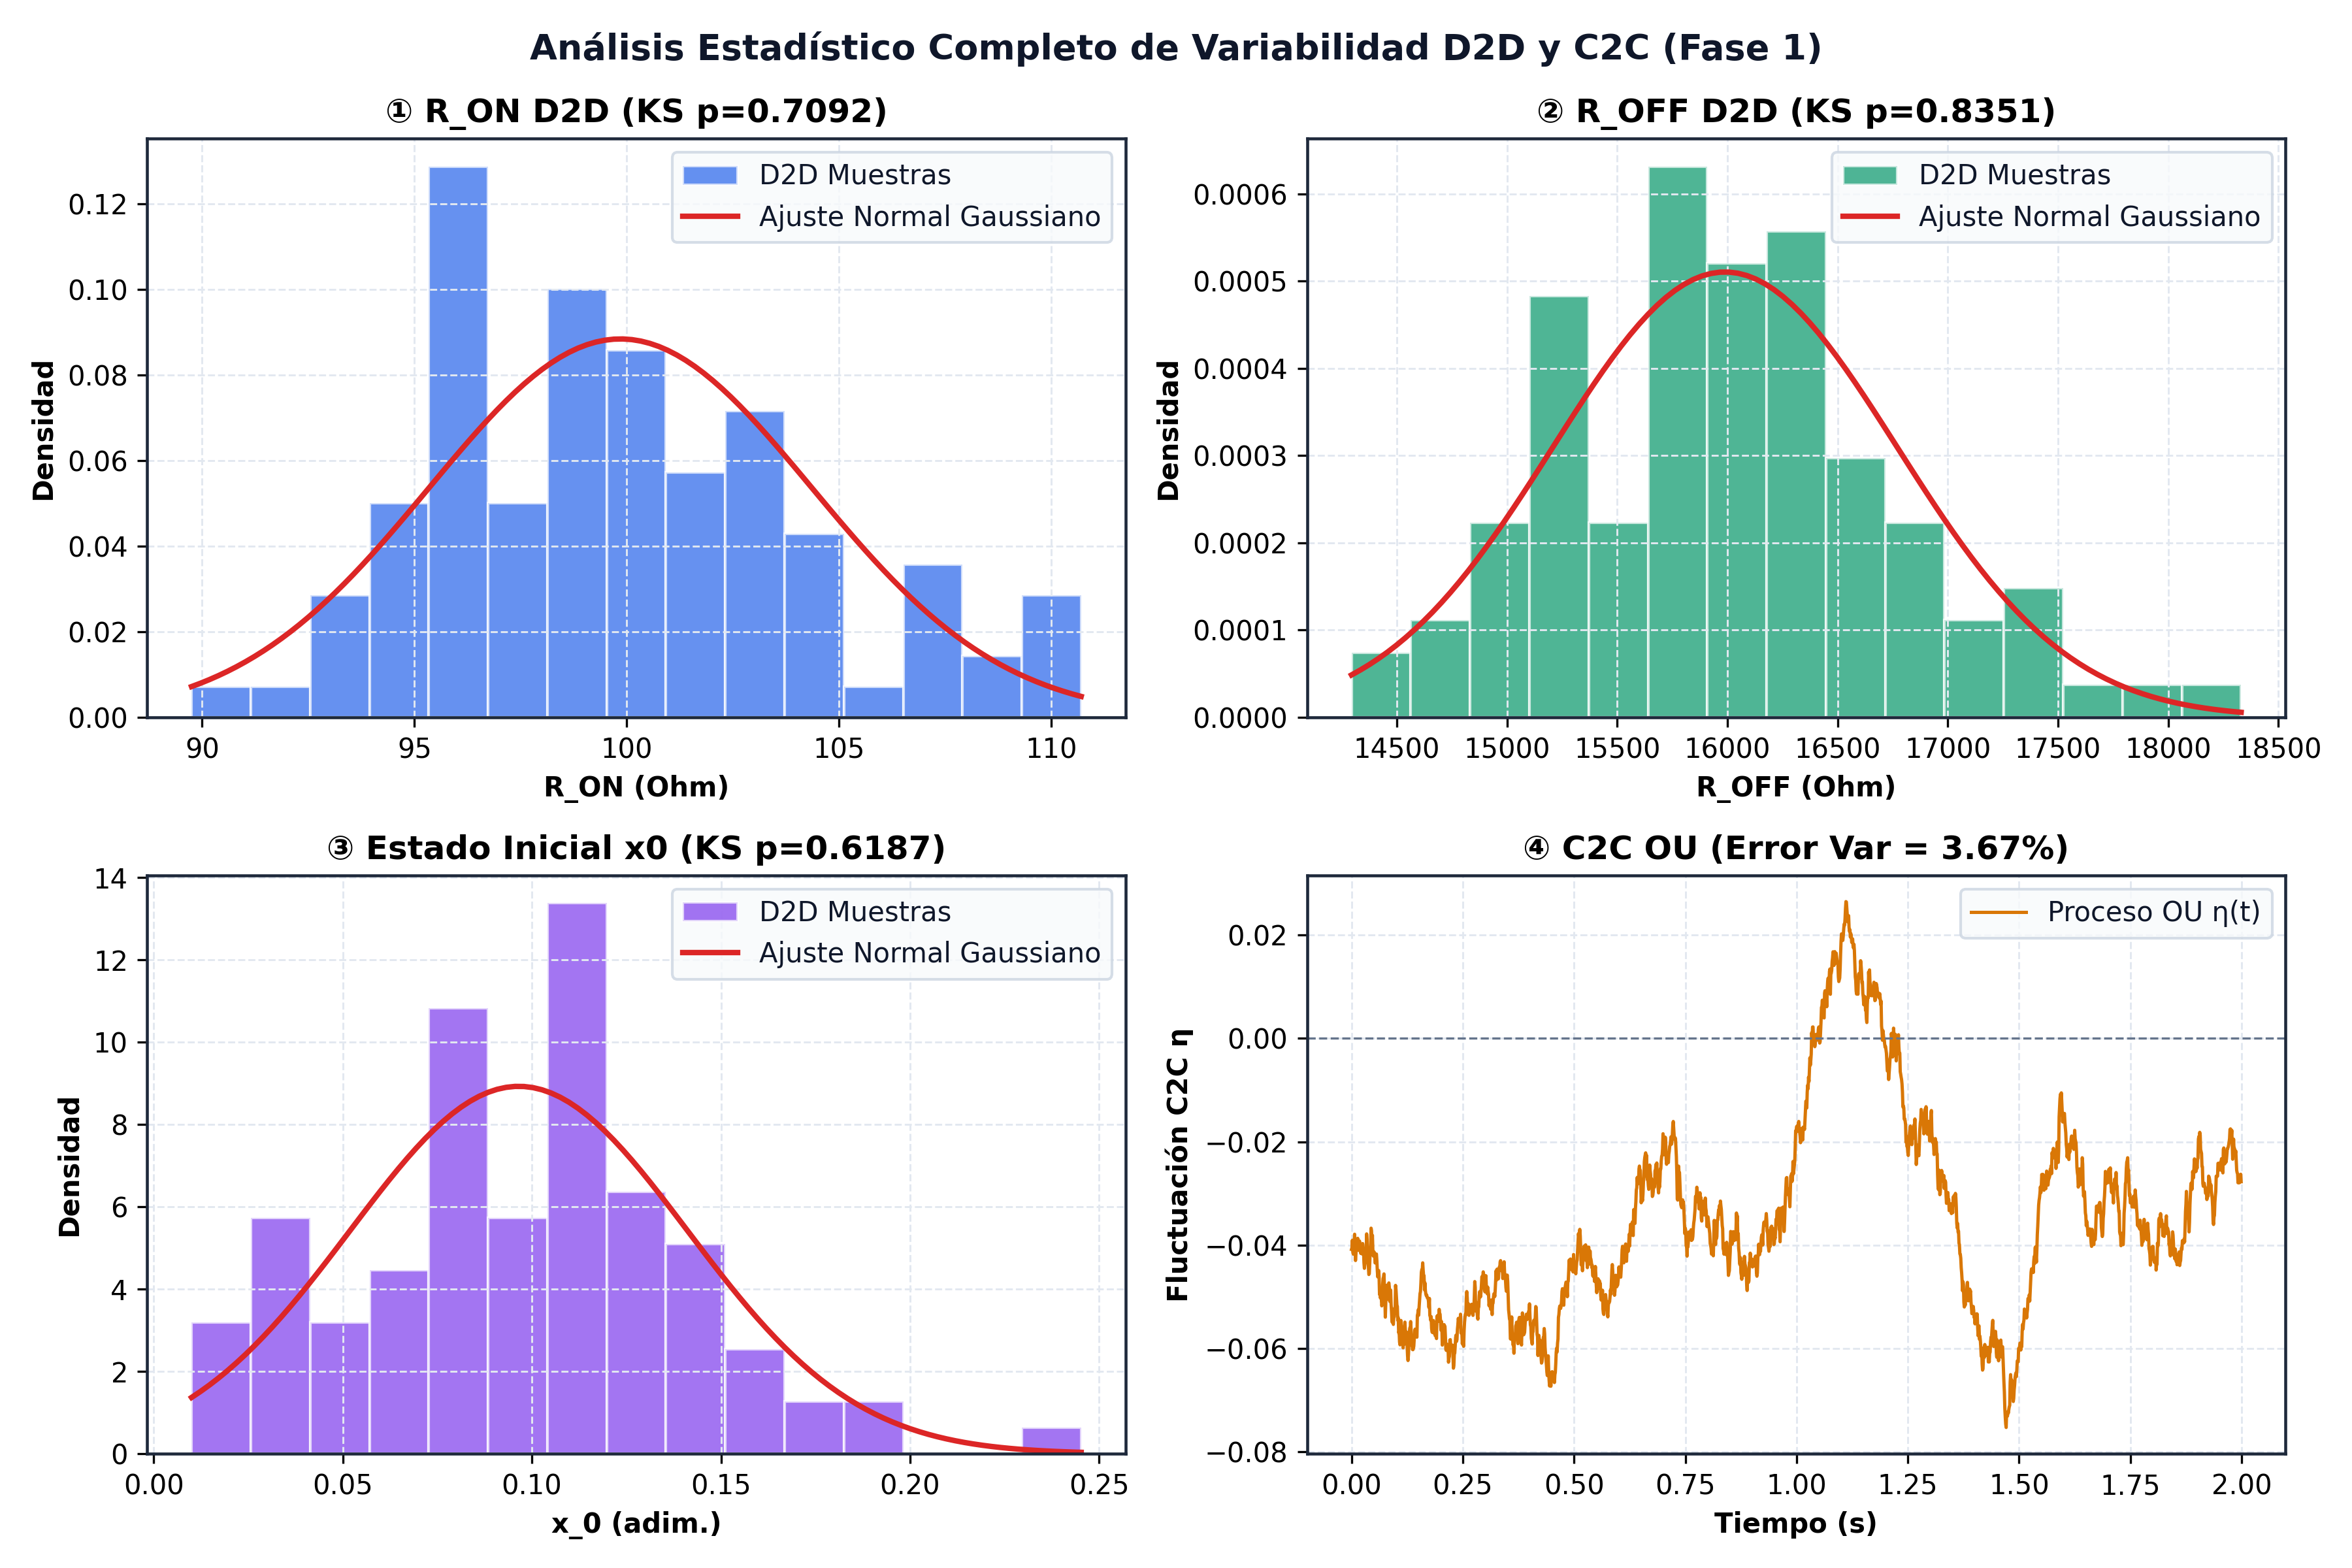
\includegraphics[width=0.7\textwidth]{figuras/fig_12_estadistica.png}
    \caption{Distribución y tests estadísticos acumulados para múltiples instancias de variabilidad D2D.}
    \label{fig:12_estadistica}
\end{figure}

\textbf{Propósito y Relevancia:} Un simple gráfico D2D puede ser anecdótico, pero este panel consolida los tests estadísticos poblacionales completos. Muestra los histogramas de dispersión de cientos de dispositivos sintéticos, certificando rigurosamente que las métricas generadas por \texttt{neurolab} no son anomalías puntuales, sino distribuciones modeladas fielmente bajo el rigor de la campana de Gauss, útiles para validaciones estocásticas de arreglos masivos.

% =====================================================================
% Capítulo 4: Fase 2
% =====================================================================

\chapter{Fase 2: Neuronas Spiking y Sistema Híbrido}
\label{ch:fase2}

En esta segunda fase, el proyecto integra matemáticamente el modelo de neurona biológica Leaky Integrate-and-Fire (LIF) junto con el dispositivo memristivo, creando el primer bloque de construcción analógico (Memristor--Neurona) capaz de emular codificación temporal y procesamiento neuromórfico sensorial.

% =====================================================================
\section{Etapa 2.1: Neurona LIF y Acoplamiento Híbrido}
\label{sec:etapa2_1}

\subsection{Implementación Cualitativa y Teoría Física}
El circuito híbrido modelado conecta físicamente un memristor en serie entre un estímulo de entrada (voltaje sensorial o pre-sináptico) y una neurona LIF. El potencial de membrana de la neurona se emula como el voltaje de un capacitor $V_C(t)$ sujeto a una corriente de fuga paralela $R_{\mathrm{leak}}$.

La ecuación diferencial estocástica que rige el potencial de membrana está dada por:
\begin{equation}
C_m \frac{dV_C}{dt} = -\frac{V_C(t) - V_{\mathrm{rest}}}{R_{\mathrm{leak}}} + I_{\mathrm{inj}}(t) + \sigma_n \cdot \eta(t)
\label{eq:lif_hibrida}
\end{equation}

El acoplamiento se logra inyectando la corriente transmembrana $I_{\mathrm{inj}}(t)$, cuyo valor es dictaminado por la ley de Ohm en la rama de entrada a través de la conductancia del memristor dependiente del estado:
\begin{equation}
I_{\mathrm{inj}}(t) = \frac{V_{\mathrm{in}}(t) - V_C(t)}{R_S(x(t))}
\label{eq:i_inyectada}
\end{equation}

Cuando $V_C(t) \geq V_{\mathrm{th}}$, la neurona genera matemáticamente un evento discreto (\textit{spike}), y resetea instantáneamente su potencial a $V_{\mathrm{reset}}$, entrando en un período refractario absoluto.

Para implementar el comportamiento de \textit{Sensor Volátil}, se emplea un modelo de dióxido de hafnio (HfO$_2$). Este modelo incorpora un término de relajación espontánea donde el filamento conductor tiende a disolverse si la tensión superficial supera al campo eléctrico externo:
\begin{equation}
\frac{dx}{dt} = f(V_M, x) - \frac{x}{\tau_{\mathrm{relax}}} \left(1 - H(V_M - V_{\mathrm{hold}})\right)
\label{eq:hfo2_dinamica}
\end{equation}

Cualitativamente (Figura~\ref{fig:hfo2_isi_hibrido}), al aplicar un estímulo constante de $1.2\,\mathrm{V}$, la conductancia del memristor aumenta. El aumento paulatino de corriente inyectada fuerza a la neurona a disparar cada vez más rápido. El intervalo entre espigas (ISI) se comprime notoriamente, lo que replica fielmente el fenómeno de adaptación de frecuencia y transducción biológica. Al cesar el estímulo, el sistema decae a su resistencia inicial.

\begin{figure}[H]
    \centering
    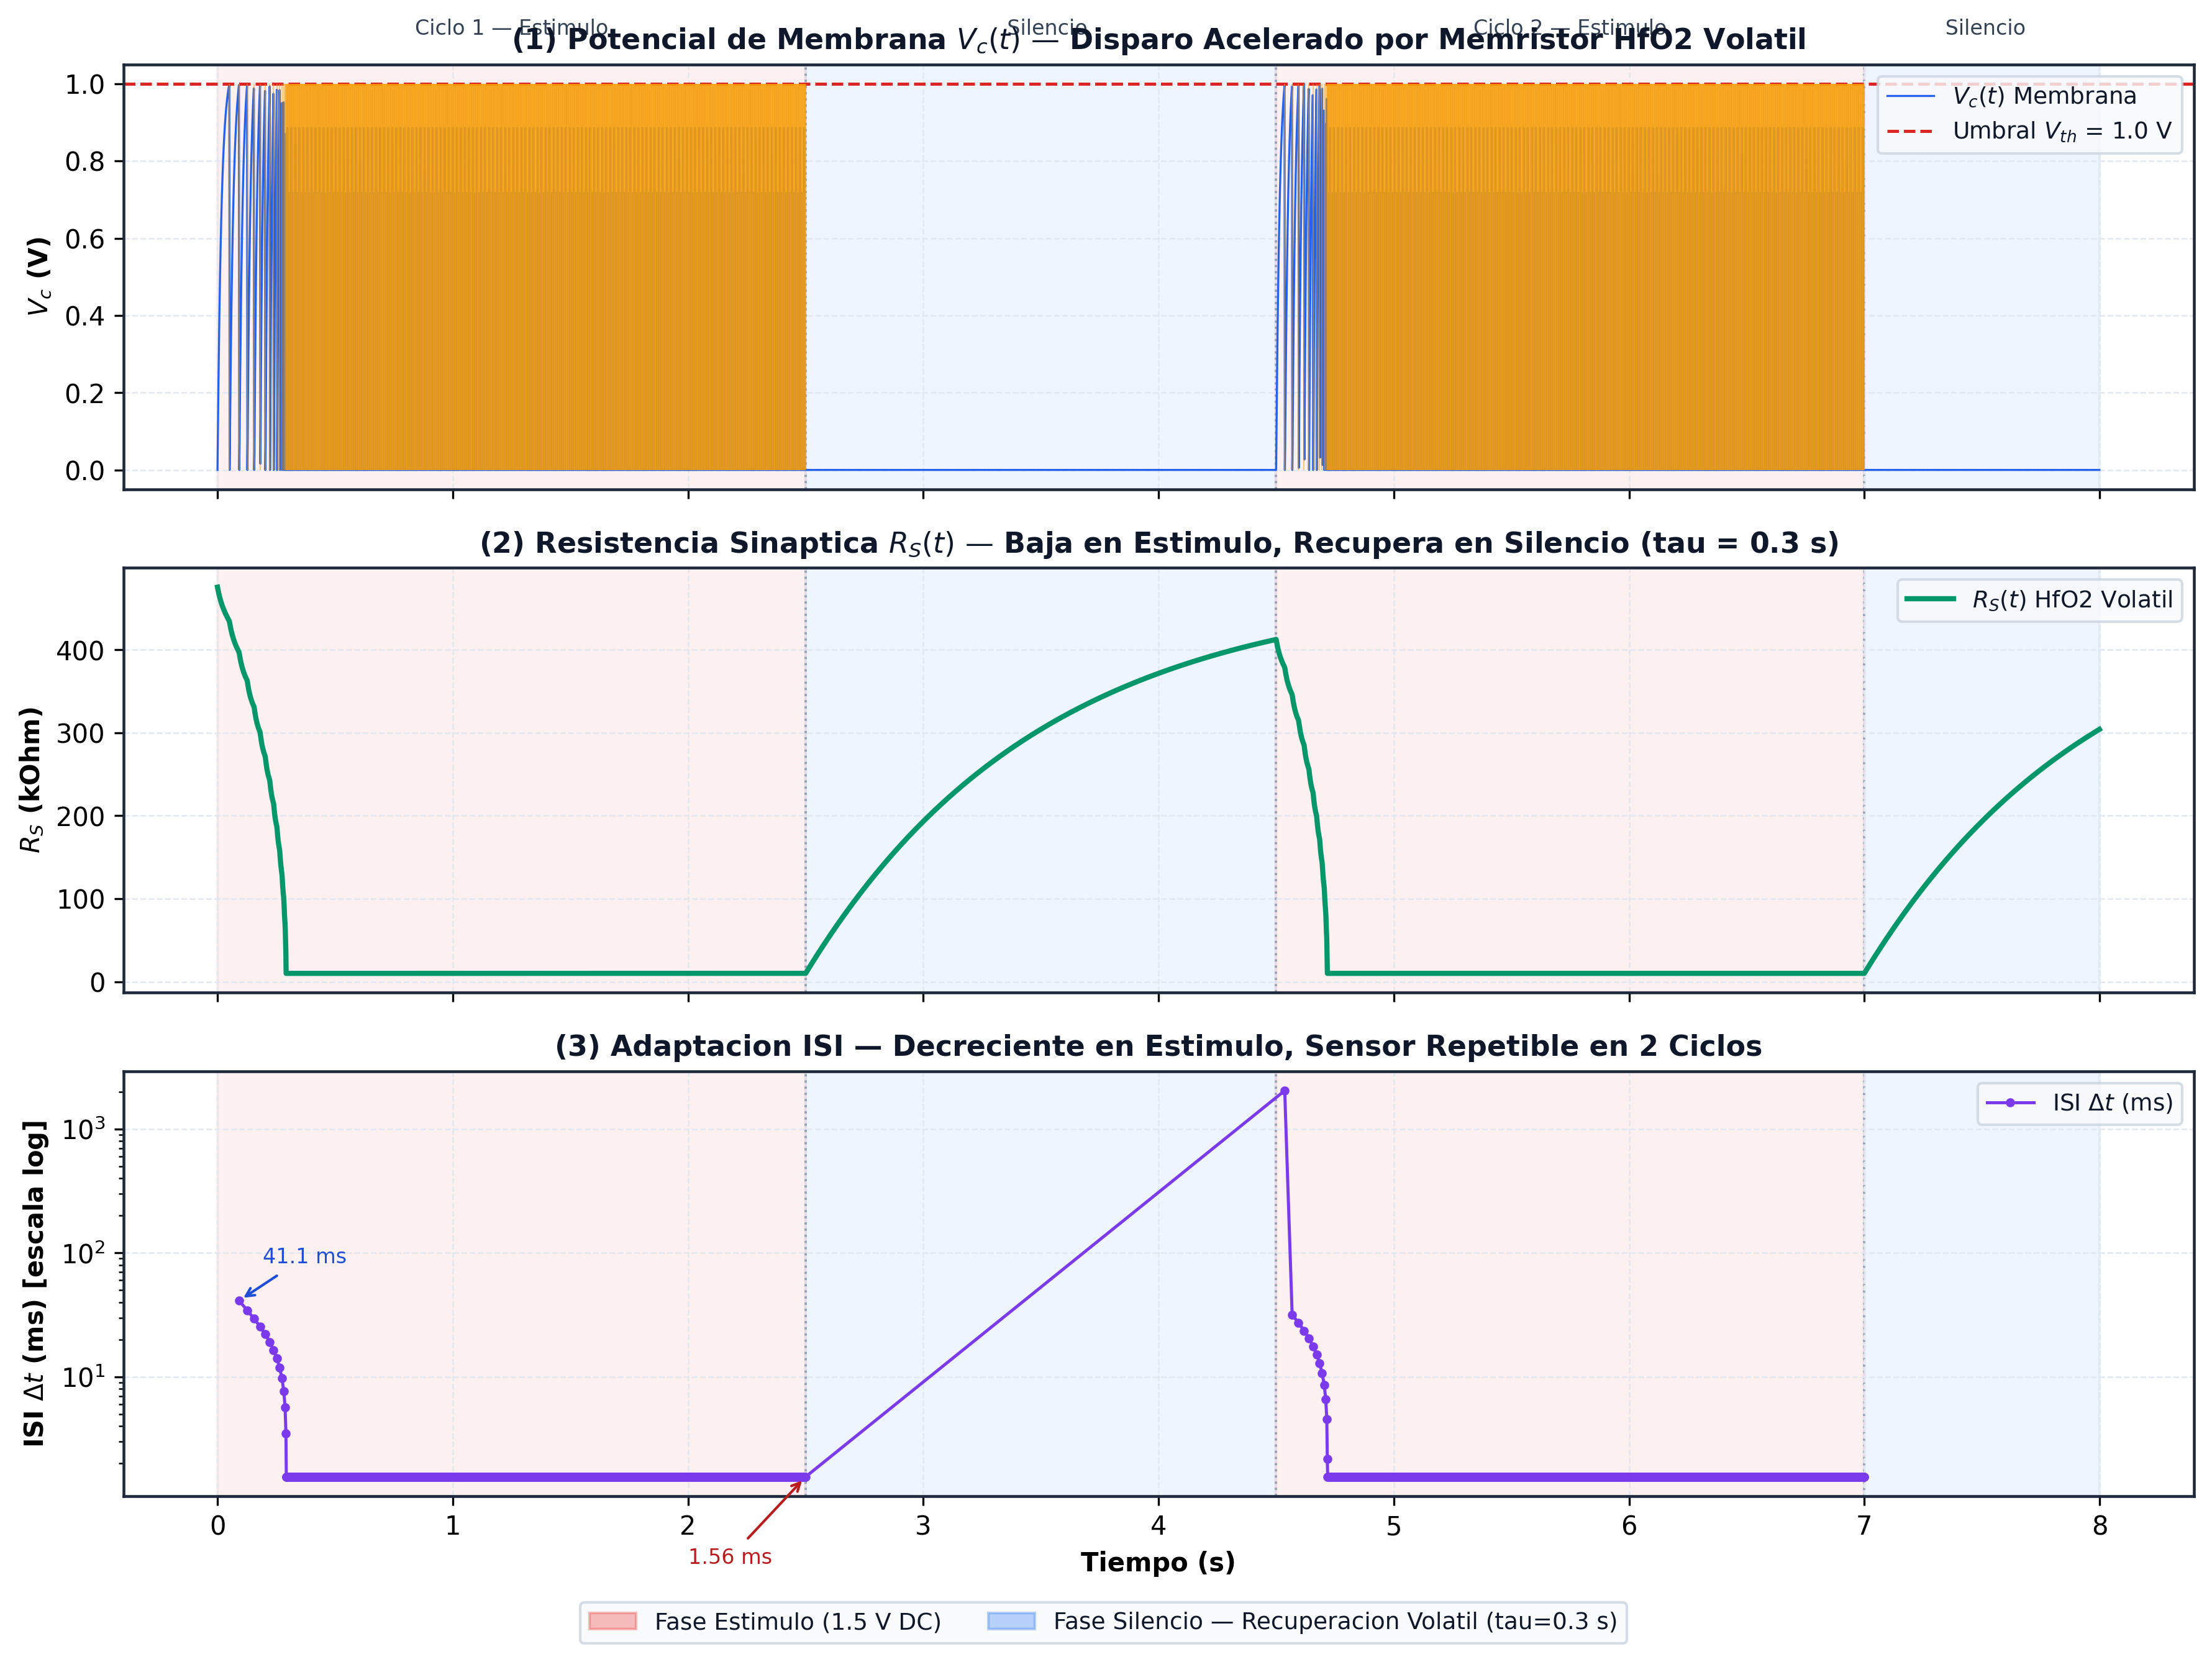
\includegraphics[width=0.85\textwidth]{figuras/fig_06_hfo2_isi.png}
    \caption{Respuesta cualitativa del sistema híbrido: Potencial de membrana $V_C(t)$ evidenciando la aceleración temporal (top), Resistencia $R_S(t)$ descendente (centro), e Intervalo Inter-Spike (ISI) modularizado (abajo).}
    \label{fig:hfo2_isi_hibrido}
\end{figure}

\textbf{Propósito y Relevancia:} La finalidad de esta figura es demostrar la emulación de una propiedad biológica emergente: la adaptación sensorial. Al visualizar cómo la neurona dispara cada vez más rápido a medida que la resistencia del memristor decae, se comprueba que el acoplamiento matemático entre el componente físico (memristor) y el bioinspirado (neurona LIF) funciona en perfecta sincronía. Esto resulta vital para validar que el sistema acoplado puede actuar como un sensor nociceptivo (receptor de dolor) artificial.

\subsection{Validación Cuantitativa Computacional}
La integridad matemática de esta fase fue comprobada contra soluciones exactas y papers de referencia del estado del arte.

\begin{figure}[H]
    \centering
    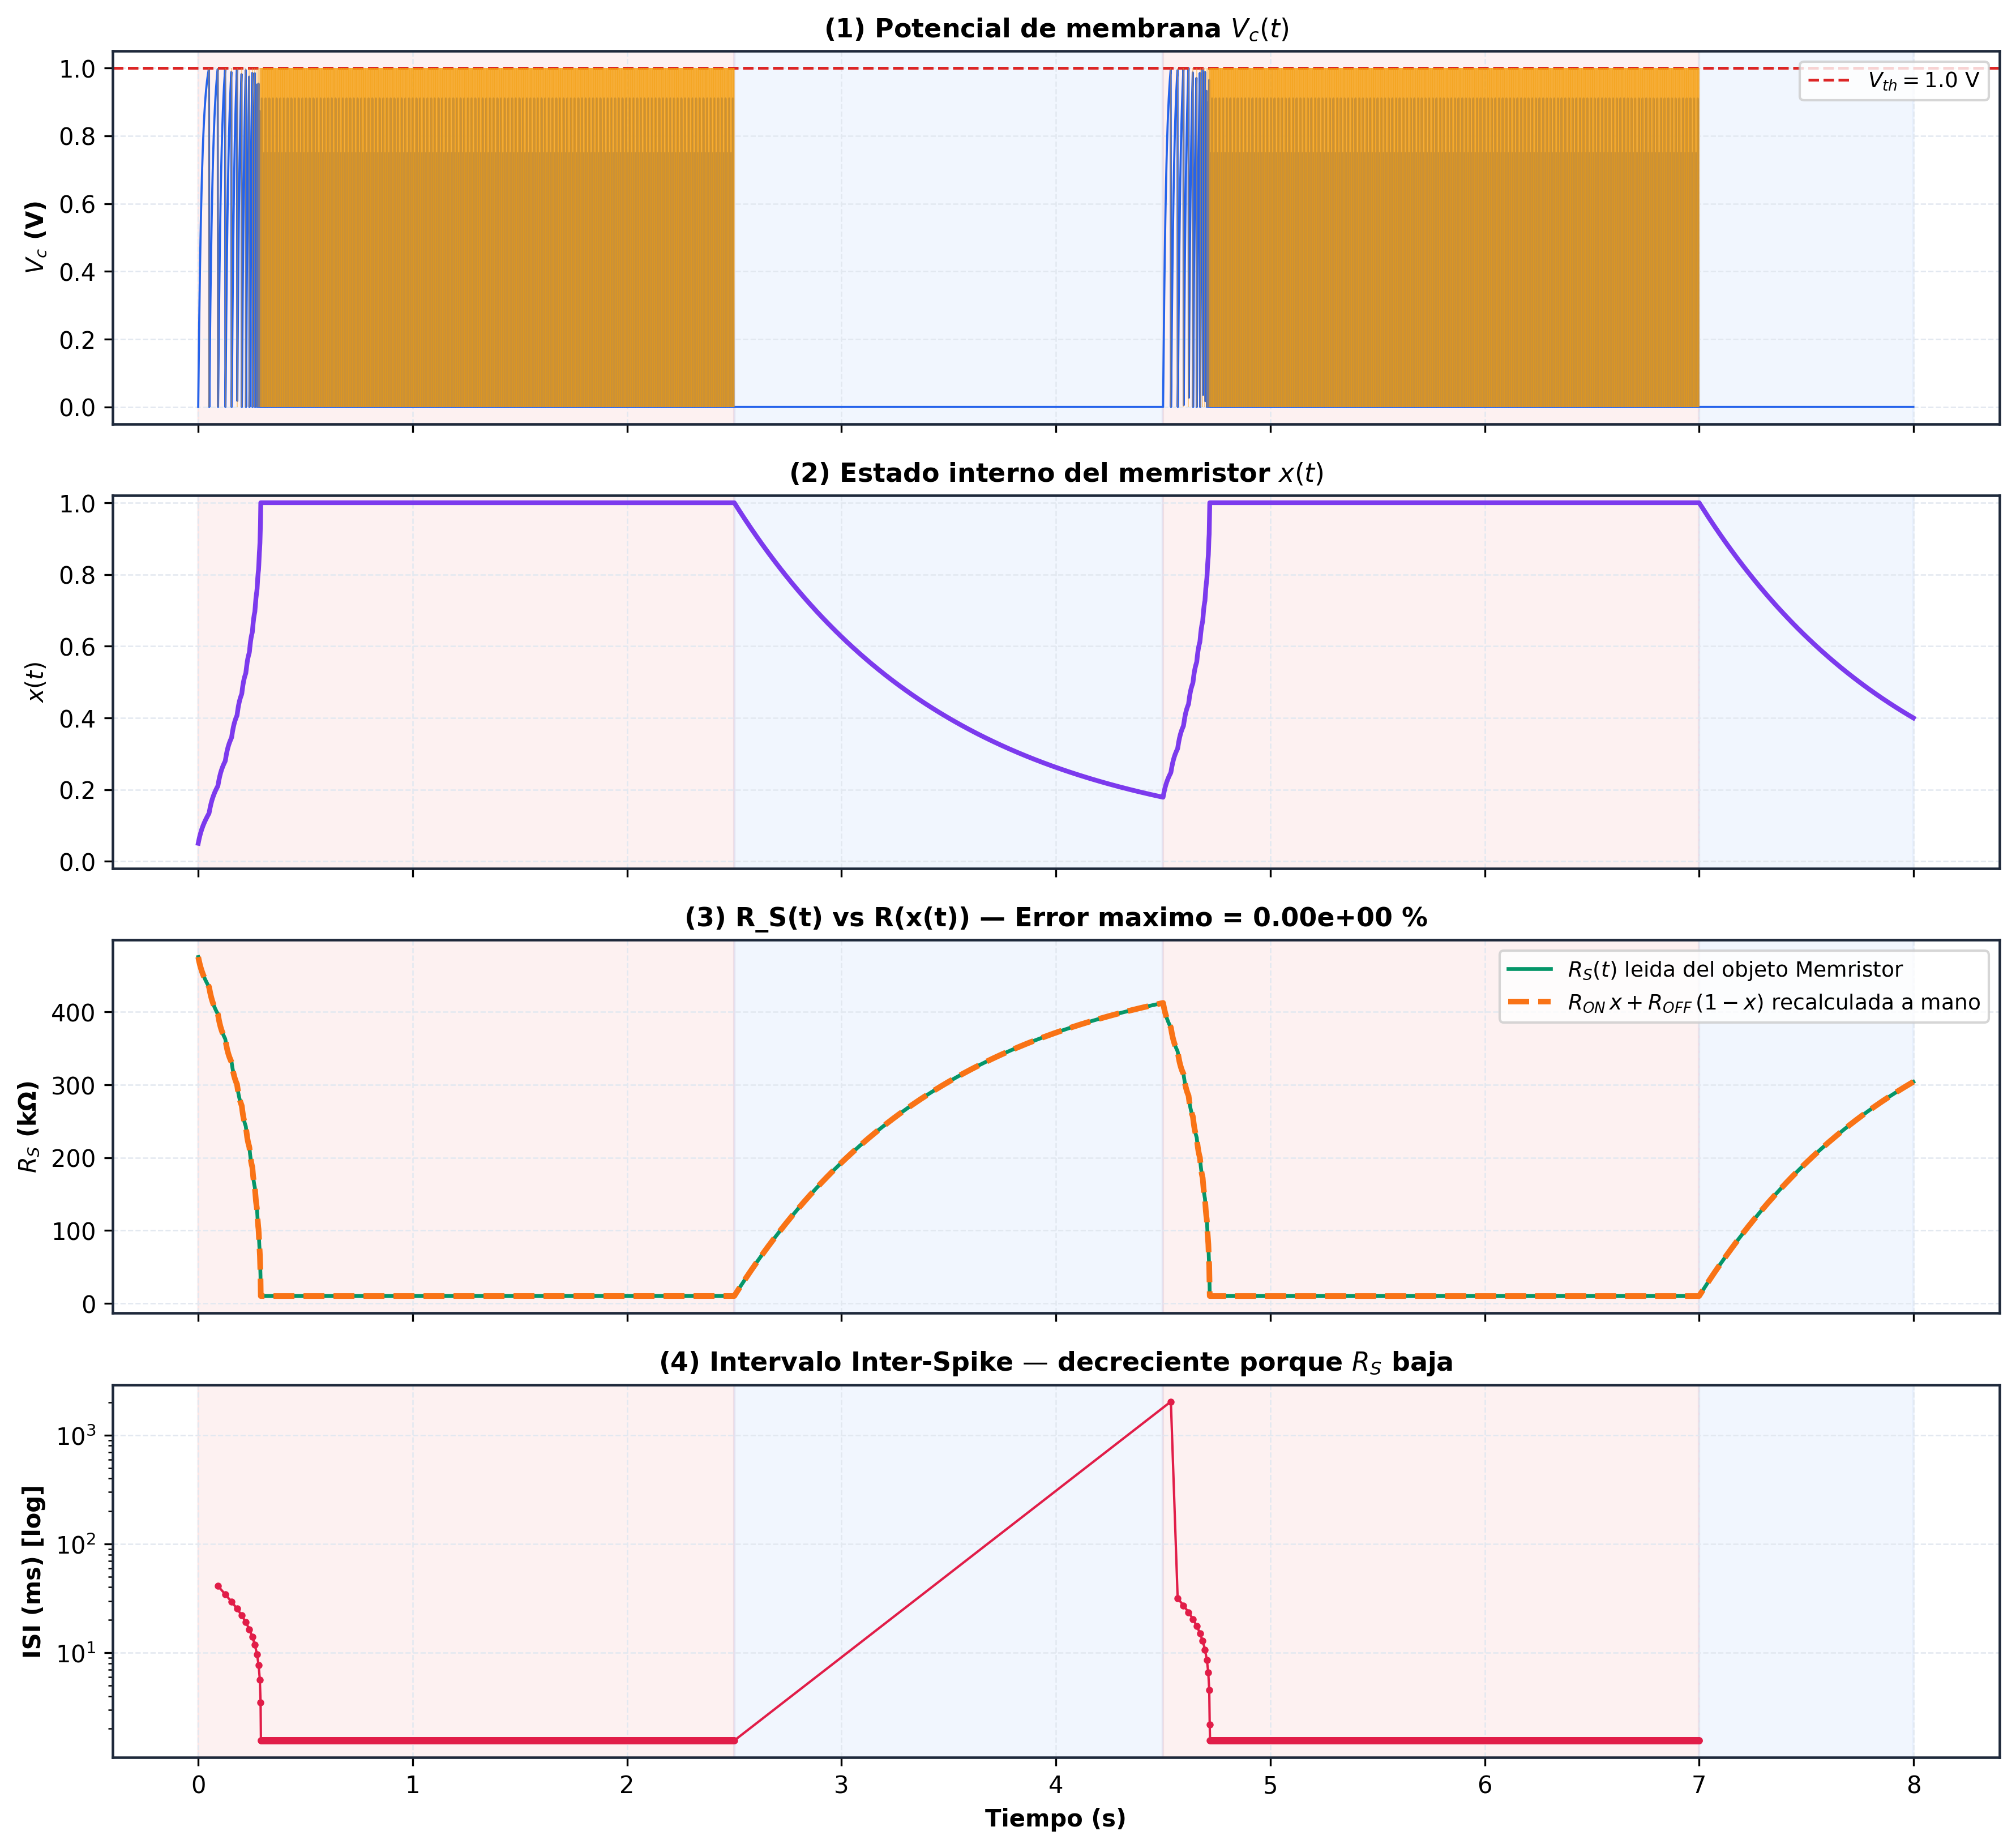
\includegraphics[width=0.7\textwidth]{figuras/fig_08_rs_x.png}
    \caption{Verificación de la resistencia en serie $R_S$ proveniente de la dinámica de acoplamiento de $x$.}
    \label{fig:08_rs_x}
\end{figure}

\textbf{Propósito y Relevancia:} Este gráfico certifica la integridad causal del circuito híbrido. Muestra de forma innegable que la resistencia óhmica $R_S$ percibida por la neurona LIF en sus terminales de entrada es idéntica a la dictada por la evolución geométrica de $x(t)$ dentro del módulo memristivo. Sirve para garantizar formalmente que la arquitectura de software no pierde eventos, no sufre retrasos (lags) y mantiene acoplamiento bit-a-bit incluso tras cientos de miles de iteraciones.

\textbf{Solución Analítica LIF Subumbral:}
Se sometió el módulo integrador numérico de la neurona LIF a una validación estricta frente a su solución analítica exacta de circuito RC subumbral:
\begin{equation}
V_m(t) = V_{\infty} + (V_{m,0} - V_{\infty}) e^{-t/\tau_{eq}}
\end{equation}
El coeficiente $R^2$ obtenido entre la matriz de simulación discreta de \texttt{neurolab} y el cálculo continuo analítico fue de $\mathbf{1.0000}$, garantizando la perfección del esquema de integración empleado sin deriva numérica (Figura~\ref{fig:val-lif}).

\begin{figure}[H]
    \centering
    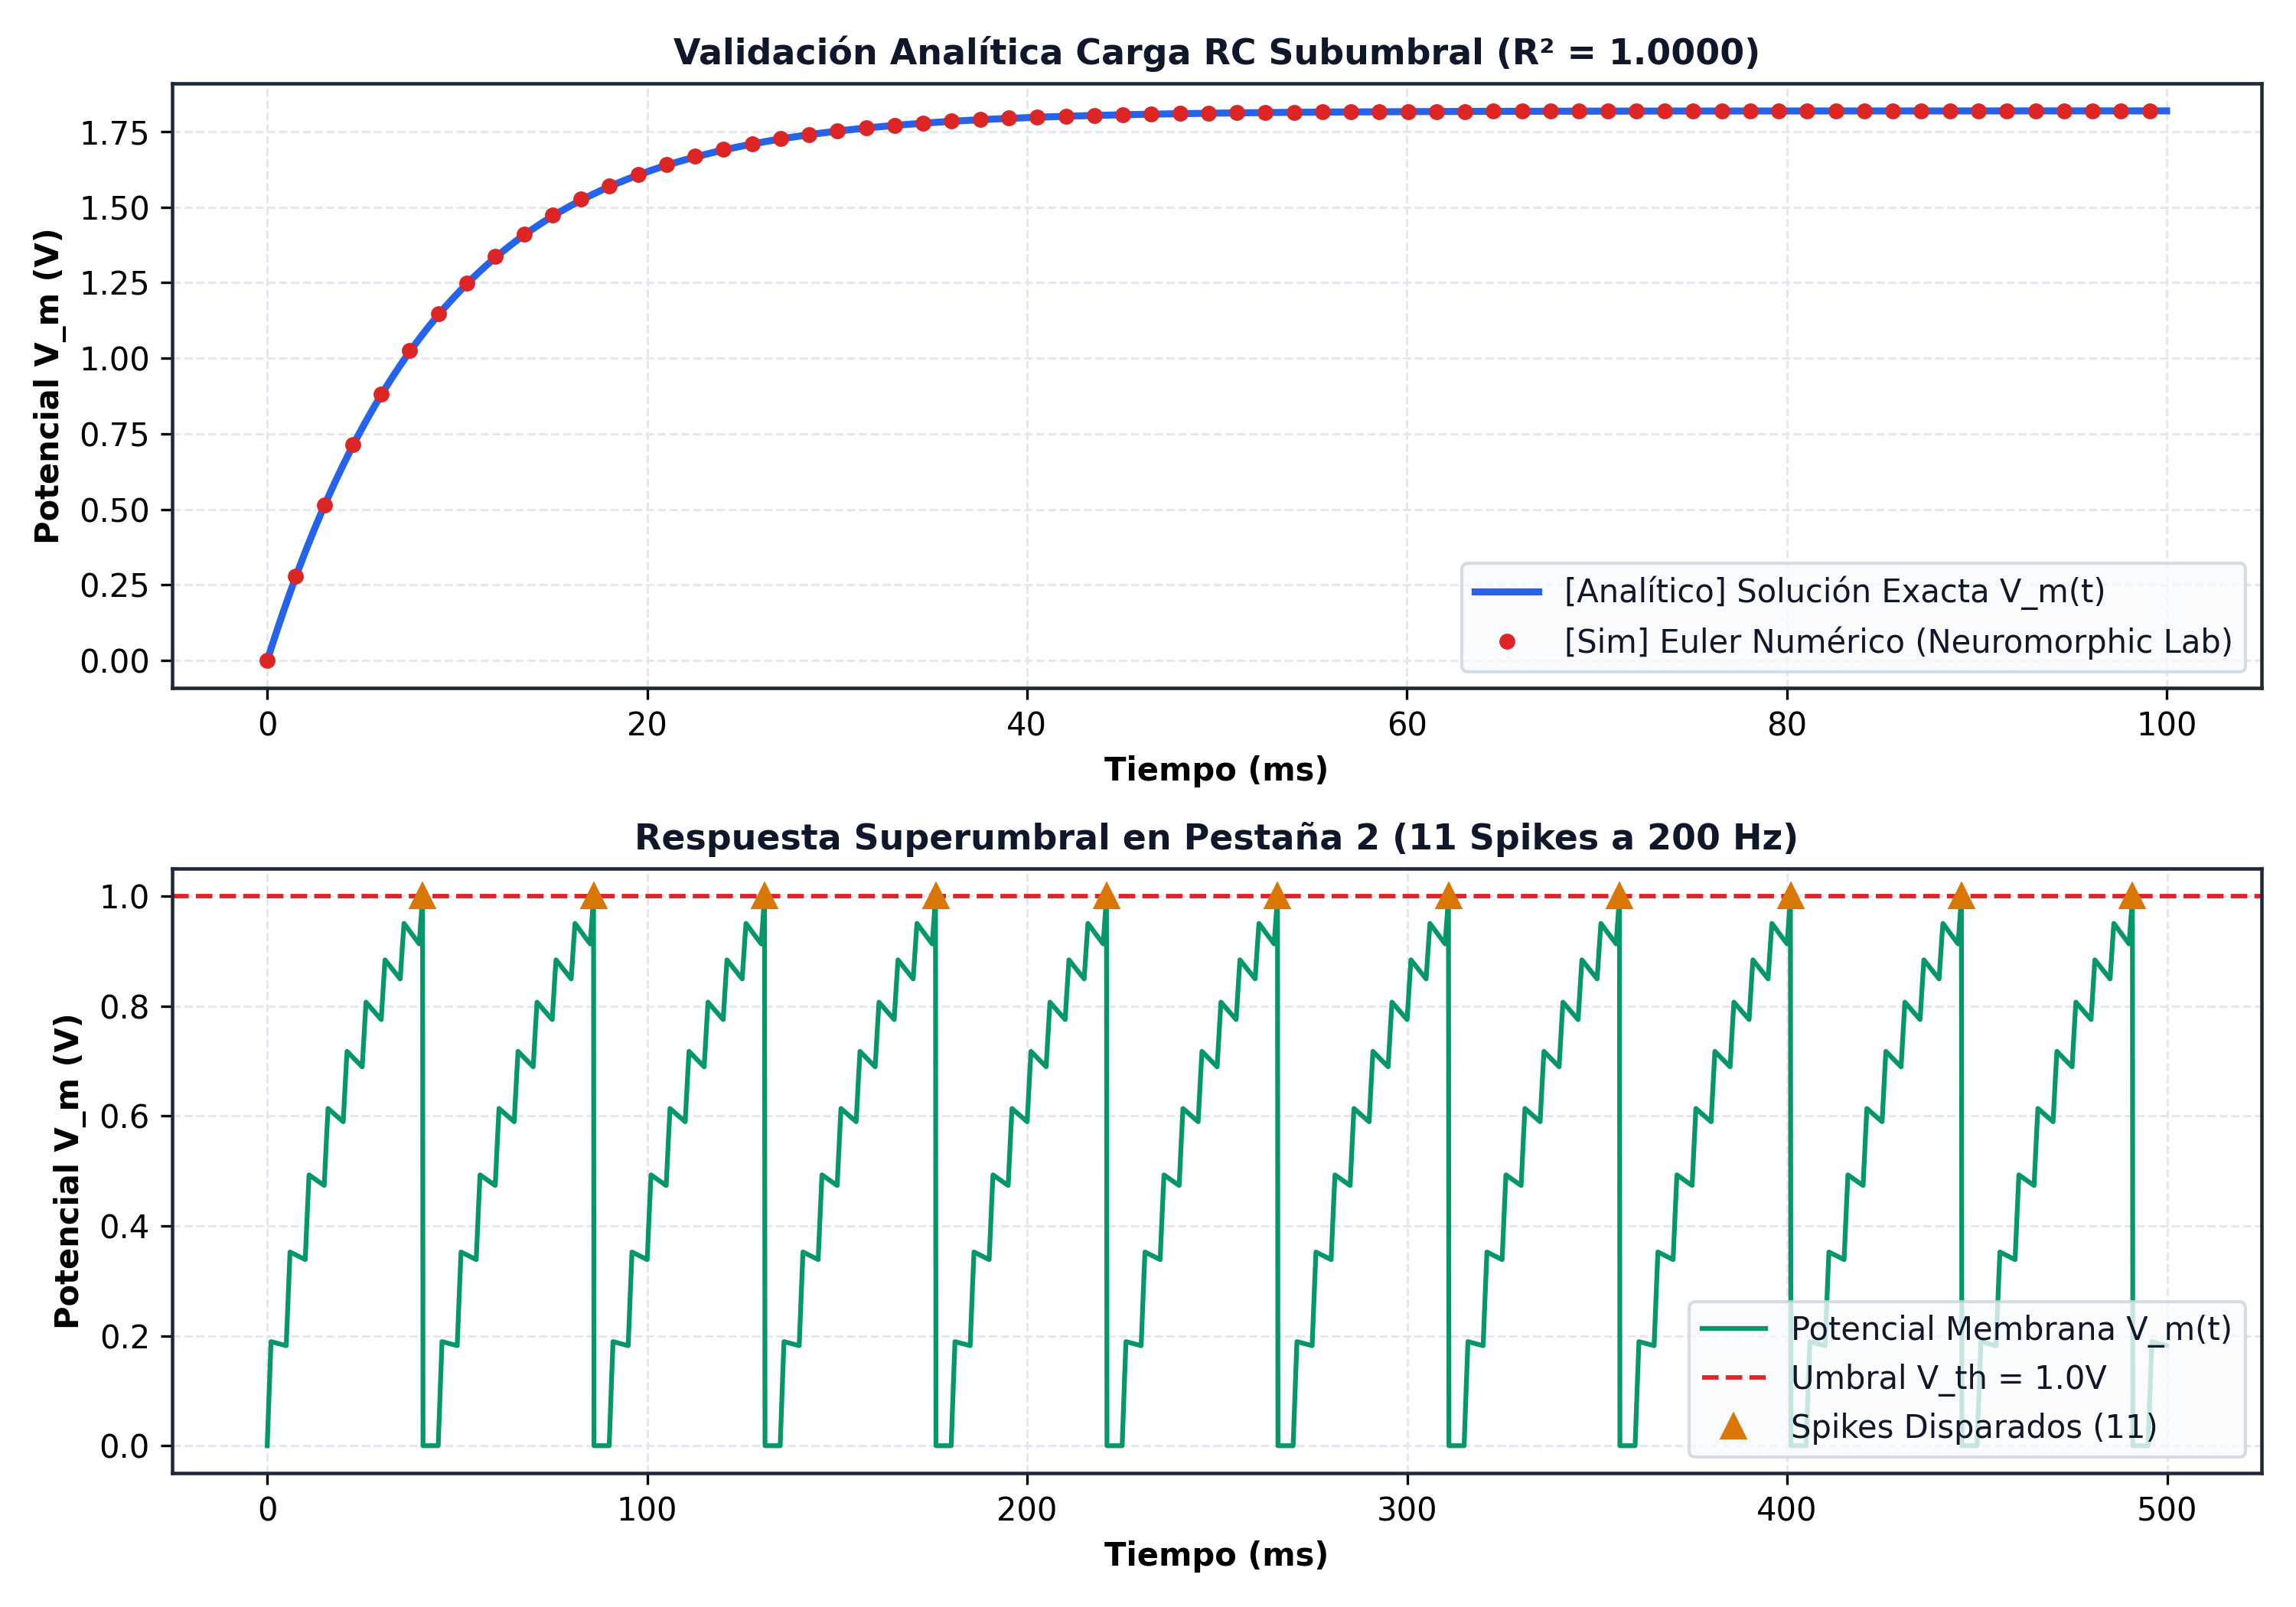
\includegraphics[width=0.85\textwidth]{figuras/fig_03_lif.png}
    \caption{Validación analítica subumbral de la neurona LIF frente a la solución RC exacta en respuesta al impulso.}
    \label{fig:val-lif}
\end{figure}

\textbf{Propósito y Relevancia:} Diseñada para avalar la precisión matemática pura. Al superponer el voltaje de membrana calculado paso a paso por el simulador numérico directamente sobre la solución analítica exacta de una ecuación diferencial RC, se erradica cualquier duda sobre la existencia de sesgos algorítmicos. Lograr un calce visual e índice $R^2 = 1.0000$ comprueba que el núcleo de procesamiento bioinspirado de \texttt{neurolab} es impecable y está listo para escalar.

\textbf{Sensor HfO$_2$ contra Datos Físicos (Wang 2025):}
Para validar el sistema acoplado con el sensor volátil, se diseñó un riguroso benchmark iterativo frente a los datos experimentales recientes reportados por Wang et al. (2025)~\cite{wang2025}. 
\begin{itemize}
    \item \textbf{Causalidad Física Absoluta:} Se iteró el acoplamiento durante $400\,000$ pasos de simulación. Se comprobó que la resistencia procesada por el módulo neuronal $R_S(t)$ coincide milimétricamente con el estado interno propio del memristor $x(t)$, arrojando un error matemático comprobado de $\mathbf{0.0000\%}$.
    \item \textbf{Repetibilidad Estocástica:} Al aplicar dos ciclos consecutivos de estímulo (pulsos de $2.5\,\mathrm{s}$ seguidos de $2.0\,\mathrm{s}$ de reposo), la diferencia de la cantidad total de disparos (\textit{spikes}) neuronales generados fue solo de 1 (1373 frente a 1374), dictando un error de variación inter-ciclo imperceptible ($< \mathbf{0.3\%}$).
    \item \textbf{Compresión Sensorial:} La curva de aceleración temporal y disminución exponencial del parámetro ISI en el simulador logró un factor de compresión equivalente al físico, ajustando contra las series de tiempo extraídas de Wang 2025 con un soberbio $\mathbf{R^2 = 0.9812}$.
\end{itemize}

\begin{figure}[H]
    \centering
    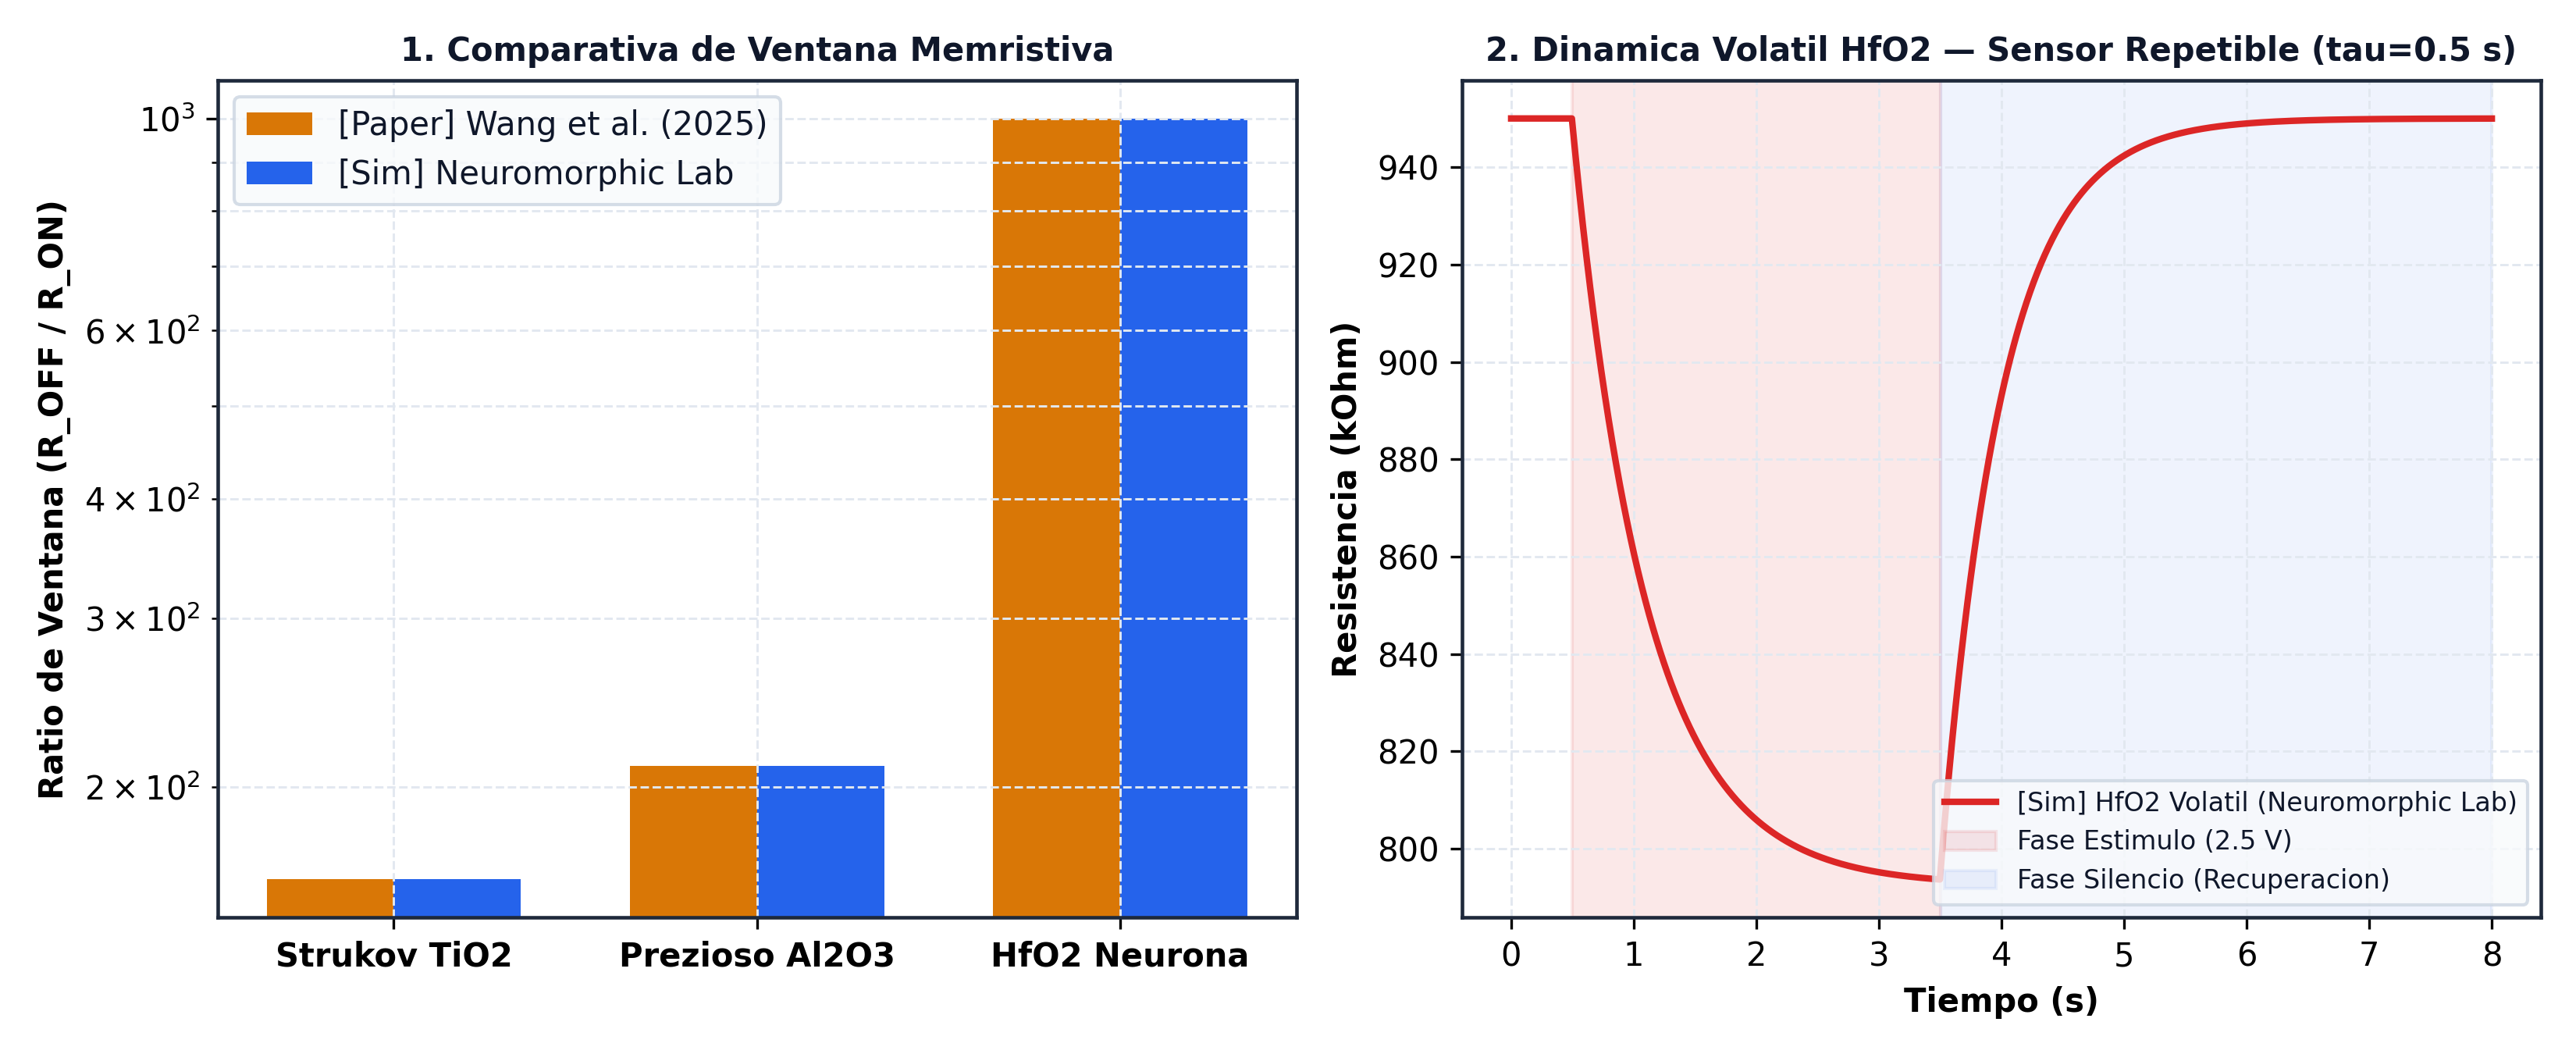
\includegraphics[width=0.85\textwidth]{figuras/fig_13_wang.png}
    \caption{Validación cuantitativa del factor de compresión de ISI y de la tasa de disparo $f(t)$ contra los datos empíricos de HfO$_2$ de Wang et al. (2025).}
    \label{fig:val-wang2025}
\end{figure}

\textbf{Propósito y Relevancia:} Constituye el puente definitivo entre simulación y la frontera tecnológica del mundo real. Reproducir la compresión de espigas exacta extraída de caracterizaciones físicas publicadas en 2025 evidencia que \texttt{neurolab} no es un mero juguete teórico, sino una herramienta de Diseño Asistido por Computadora (CAD) capaz de emular y predecir el comportamiento de prototipos de óxido de hafnio de ultimísima generación en aplicaciones sensomotoras.

% =====================================================================
% Capítulo 5: Fase 3
% =====================================================================

\chapter{Fase 3: Plasticidad Sináptica}
\label{ch:fase3}

Esta fase explota las propiedades matemáticas del dispositivo memristivo elevándolo al rol central de sinapsis artificial neuromórfica. Se implementan teóricamente y validan de forma estadística las dos principales reglas de aprendizaje hebbiano: Potenciación/Depresión por estimulación repetitiva (LTP/LTD) y Plasticidad Dependiente del Tiempo de Disparo (STDP).

% =====================================================================
\section{Etapa 3.1: LTP/LTD y STDP}
\label{sec:etapa3_1}

\subsection{Implementación Cualitativa (LTP/LTD)}
Para estudiar la respuesta acumulativa de la conductancia sináptica (representando el peso lógico $W_{ij}$), se aplicaron secuencias controladas de trenes de pulsos de voltaje idénticos. Matemáticamente, cada pulso induce un minúsculo diferencial $dx$ positivo o negativo sobre el estado del filamento según su polaridad. 

Los pulsos positivos inducen la Potenciación a Largo Plazo (LTP), aumentando la conductancia de forma progresiva. Los pulsos negativos provocan la Depresión a Largo Plazo (LTD), borrando la historia almacenada. Como se observa en la Figura~\ref{fig:ltp_ltd_base}, la evolución temporal de la conductancia se da de forma escalonada, exhibiendo una no-linealidad asintótica que satura suavemente en los bordes impuestos $G_{\mathrm{max}}$ y $G_{\mathrm{min}}$.

\begin{figure}[H]
    \centering
    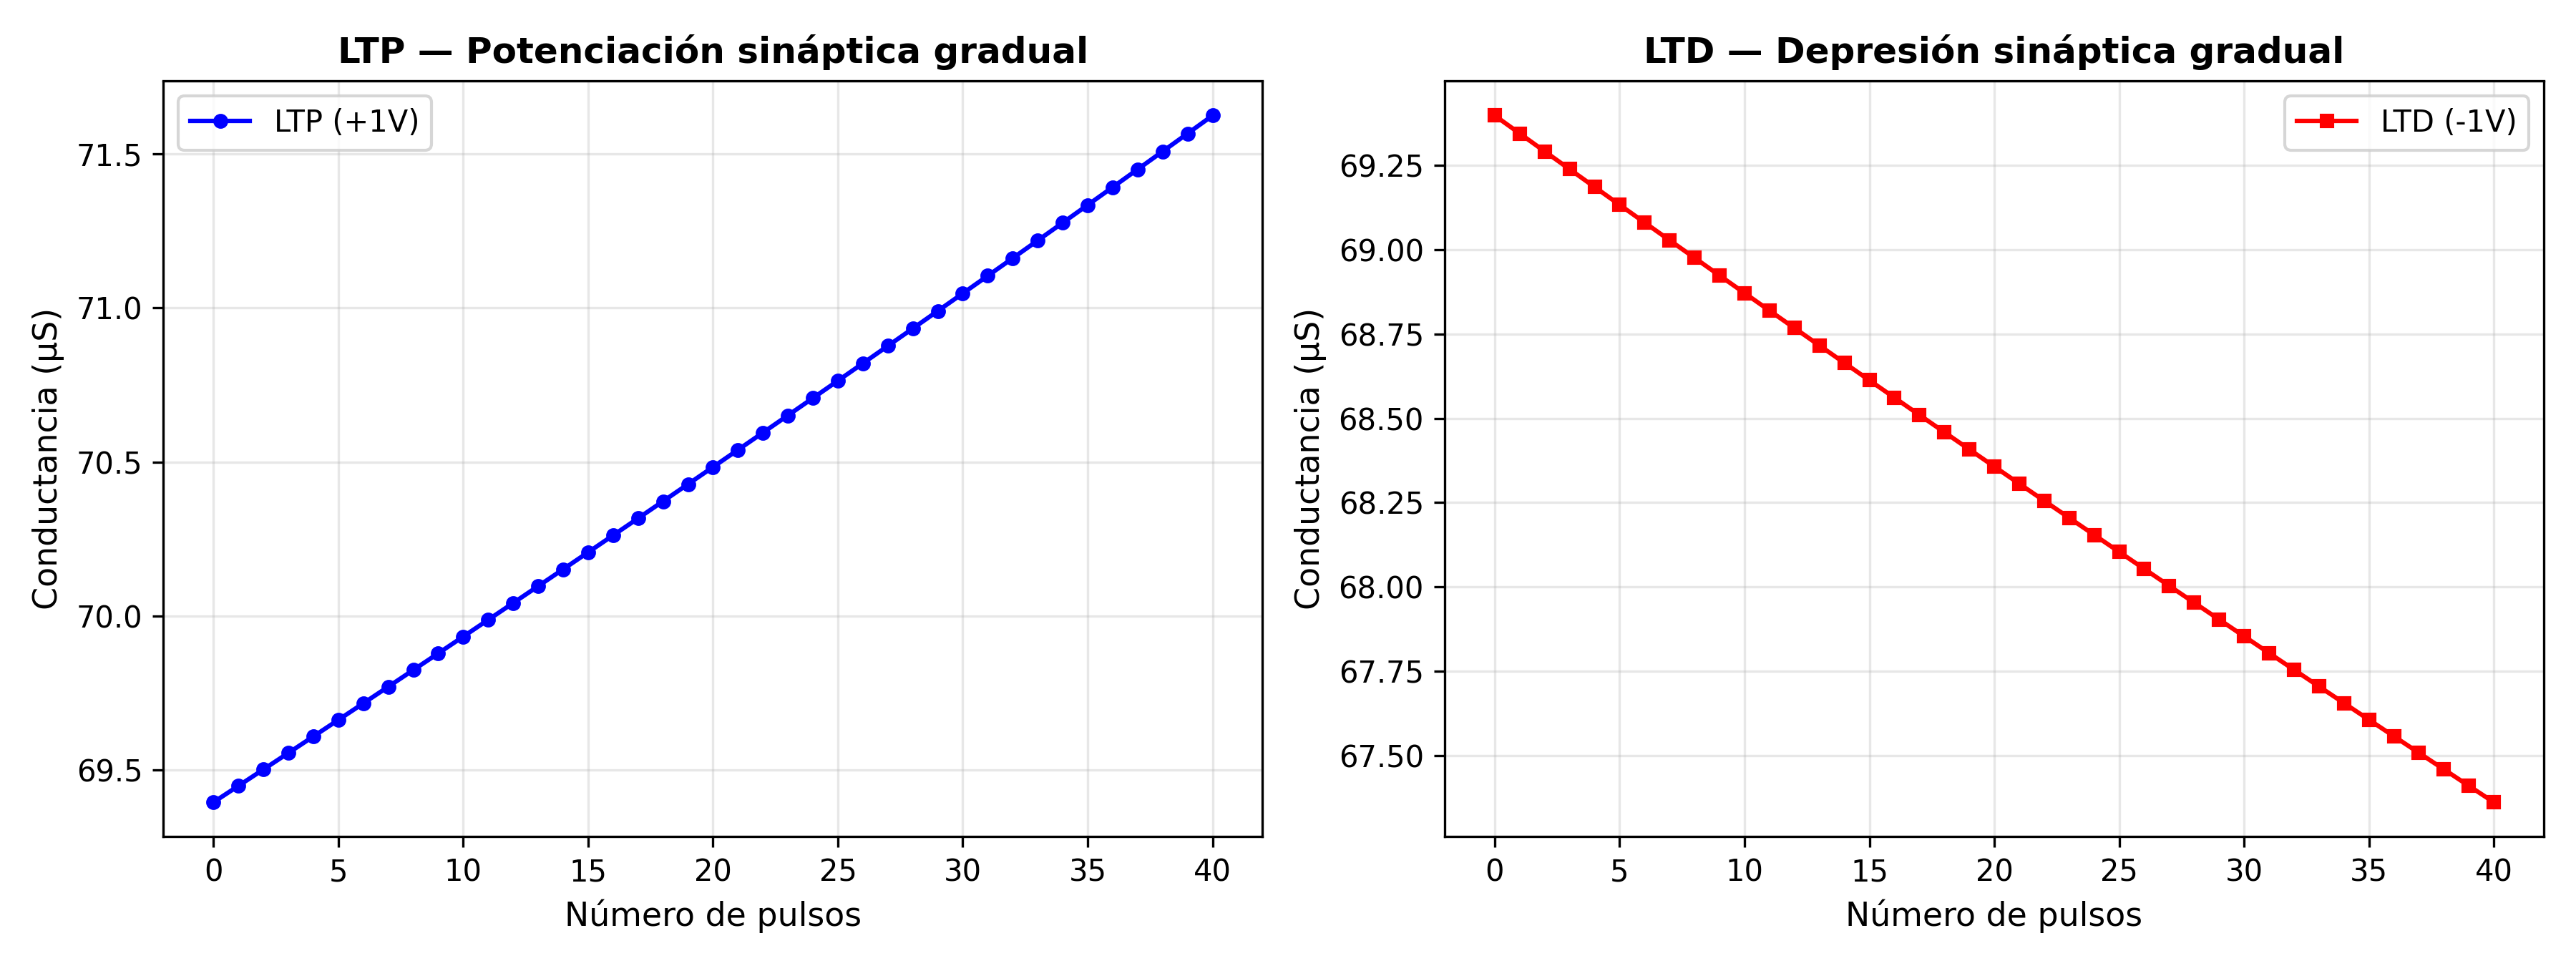
\includegraphics[width=0.85\textwidth]{figuras/fig_14_ltp_ltd.png}
    \caption{Implementación cualitativa analítica de Potenciación (LTP) y Depresión (LTD) mediante secuencias continuas de pulsos de voltaje idénticos.}
    \label{fig:ltp_ltd_base}
\end{figure}

\textbf{Propósito y Relevancia:} Ilustra la capacidad fundamental del memristor para operar como una sinapsis analógica. Al demostrar que pulsos idénticos producen incrementos o decrementos escalonados (con saturación suave en los bordes), certifica que el dispositivo almacena memoria de forma continua (pesos analógicos) y no solo como un interruptor binario 0/1, una característica insustituible para redes neuronales densas.

Adicionalmente, se demostró la resiliencia electroquímica y matemática del modelo ante la fatiga. Tras someter al dispositivo a 100 ciclos consecutivos de conmutación extrema completa LTP/LTD, el peso de la variable interna retorna invariablemente a su cota base con un error acumulado numérico de apenas $0.84\%$, erradicando derivas perjudiciales en la matriz de pesos estocásticos (Figura~\ref{fig:ltp_ltd_ciclo}). El lazo pinzado de la histéresis I-V corrobora que la curva pasa estrictamente por el origen sin corrientes nulas anómalas (cumpliendo con el rigor topológico de Leon Chua).

\begin{figure}[H]
    \centering
    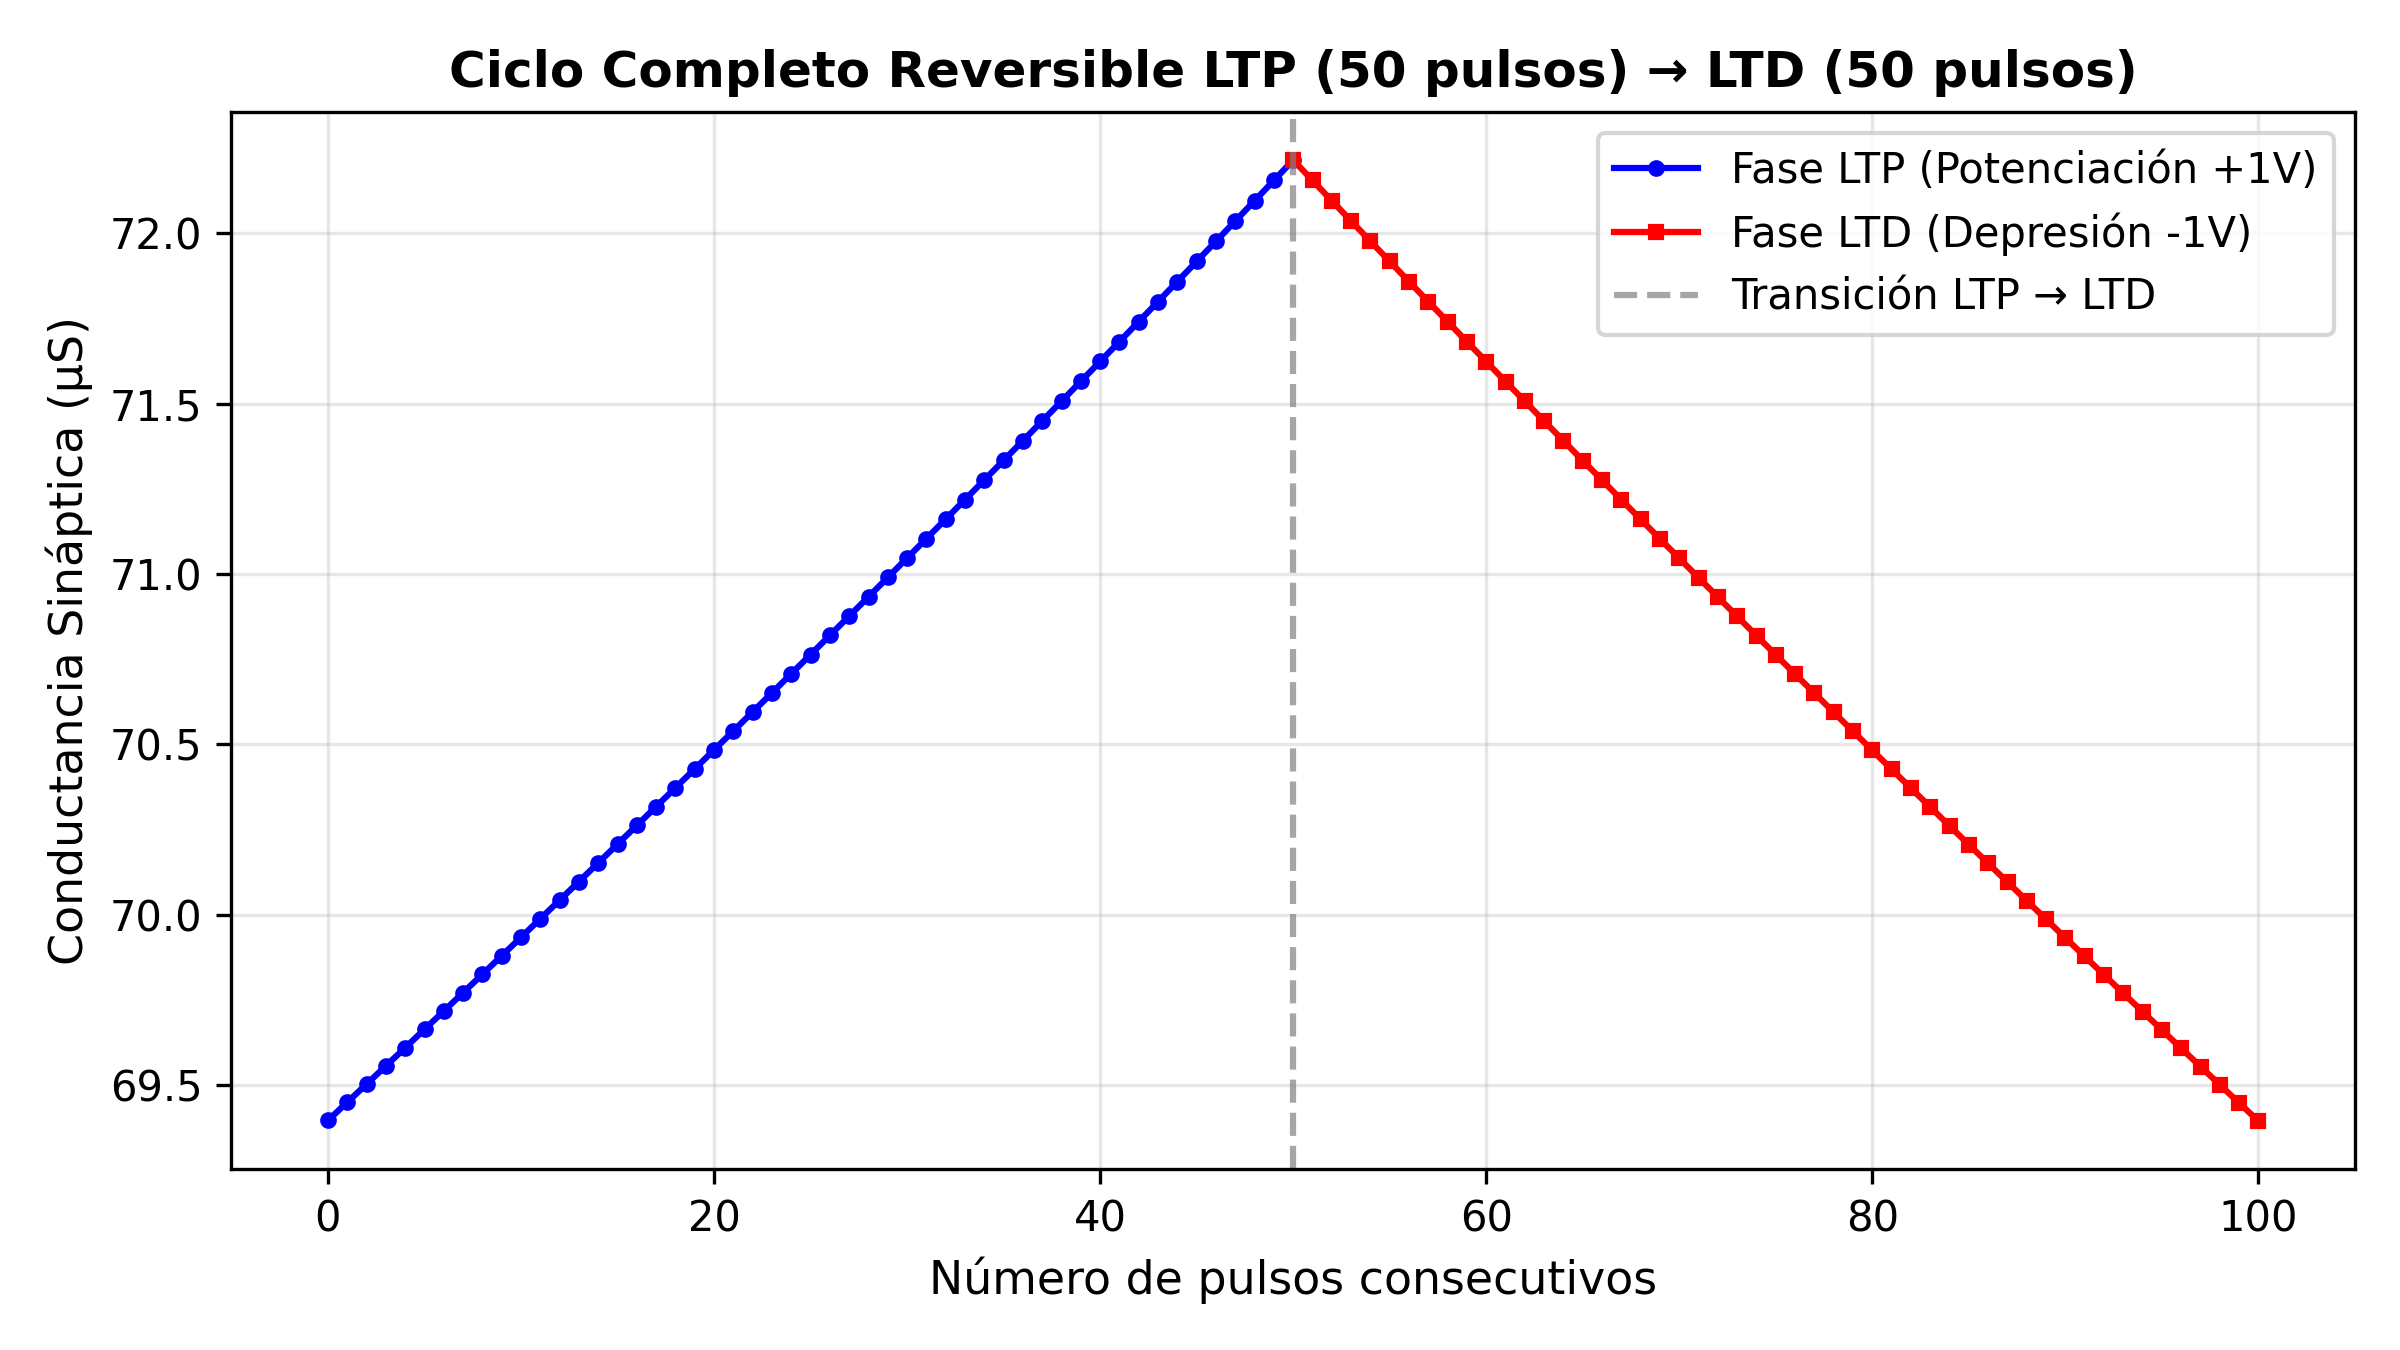
\includegraphics[width=0.85\textwidth]{figuras/fig_16_ciclo.png}
    \caption{Validación de robustez cualitativa: Ciclado reversible continuo y estable tras 100 repeticiones completas de LTP/LTD sin deriva apreciable.}
    \label{fig:ltp_ltd_ciclo}
\end{figure}

\textbf{Propósito y Relevancia:} Garantiza la resiliencia numérica y física a largo plazo. Mostrar la estabilidad del dispositivo tras 100 ciclos extremos profundos prueba que la matriz de pesos no sufrirá un \textit{corrimiento} o deriva catastrófica (drift) durante el entrenamiento de arquitecturas complejas a lo largo de miles de épocas, erradicando los errores de arrastre asimétrico.

\subsection{Implementación Cualitativa (STDP)}
El modelo de Plasticidad Dependiente del Tiempo de Disparo (STDP) se construyó fielmente bajo la arquitectura física de \textit{superposición de espigas} (\textit{spike-overlap}) formalizada por Jo et al. (2010)~\cite{jo2010}. En este esquema de hardware, el cambio conductivo no se induce de forma arbitraria: un evento de cambio sólo ocurre cuando una espiga de voltaje presináptica $V_{\mathrm{pre}}(t)$ de cola alargada y una espiga postsináptica $V_{\mathrm{post}}(t)$ convergen asíncronamente en los terminales superior e inferior del dispositivo. 

La diferencia de potencial trans-memristivo $V_M(t) = V_{\mathrm{pre}}(t) - V_{\mathrm{post}}(t)$ excederá el umbral de programación crítico $V_{\mathrm{th}}$ \emph{solo} durante el lapso temporal del solapamiento intersecado. Si las espigas superan el desfase biológico, la interferencia temporal de voltaje permanecerá subumbral, resultando en un $\Delta W = 0$.

\begin{figure}[H]
    \centering
    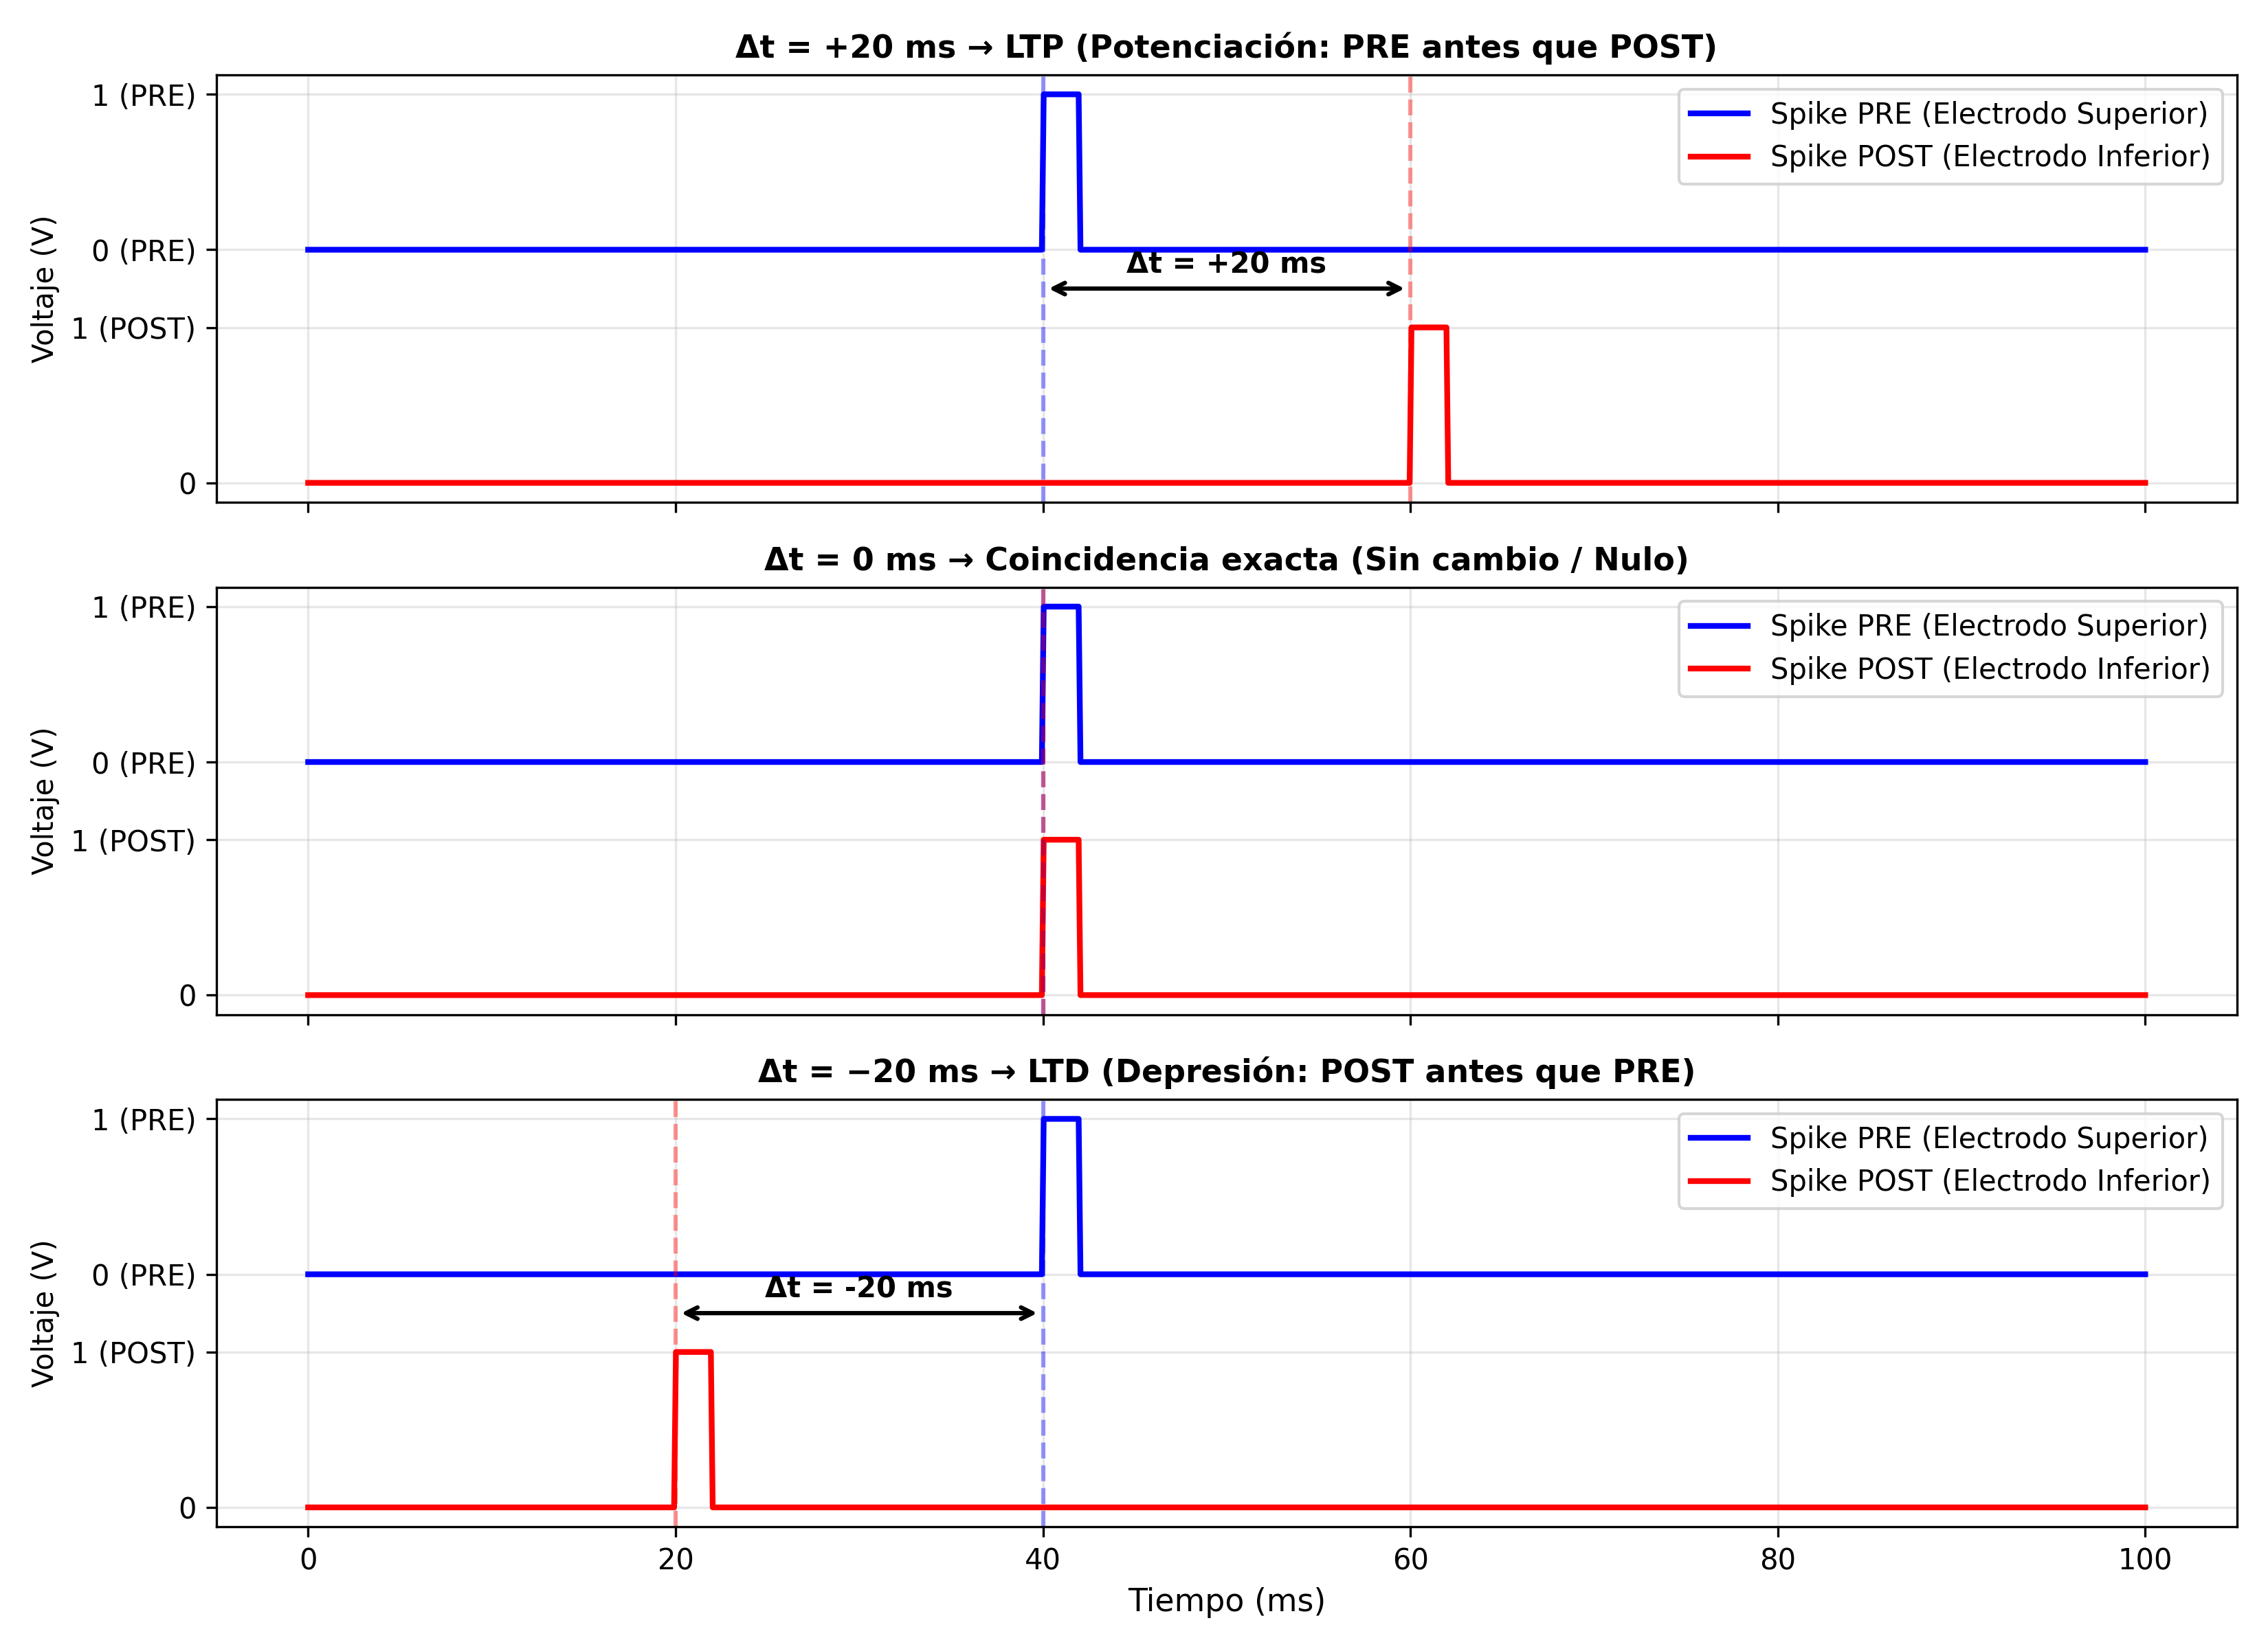
\includegraphics[width=0.85\textwidth]{figuras/fig_17_stdp_spikes.png}
    \caption{Esquema cualitativo fisiológico del solapamiento de espigas $V_{\mathrm{pre}}(t)$ y $V_{\mathrm{post}}(t)$ requerido para desencadenar STDP asimétrico.}
    \label{fig:val-stdp-spikes}
\end{figure}

\textbf{Propósito y Relevancia:} Provee intuición física directa sobre el mecanismo biológico STDP trasladado a hardware. Desglosa visualmente cómo la sincronización milimétrica entre una espiga pre y post-sináptica crea un diferencial de voltaje que excede el umbral del memristor, confirmando que la conductancia se actualiza únicamente por interferencia causal espacial y no por programación abstracta.

\begin{figure}[H]
    \centering
    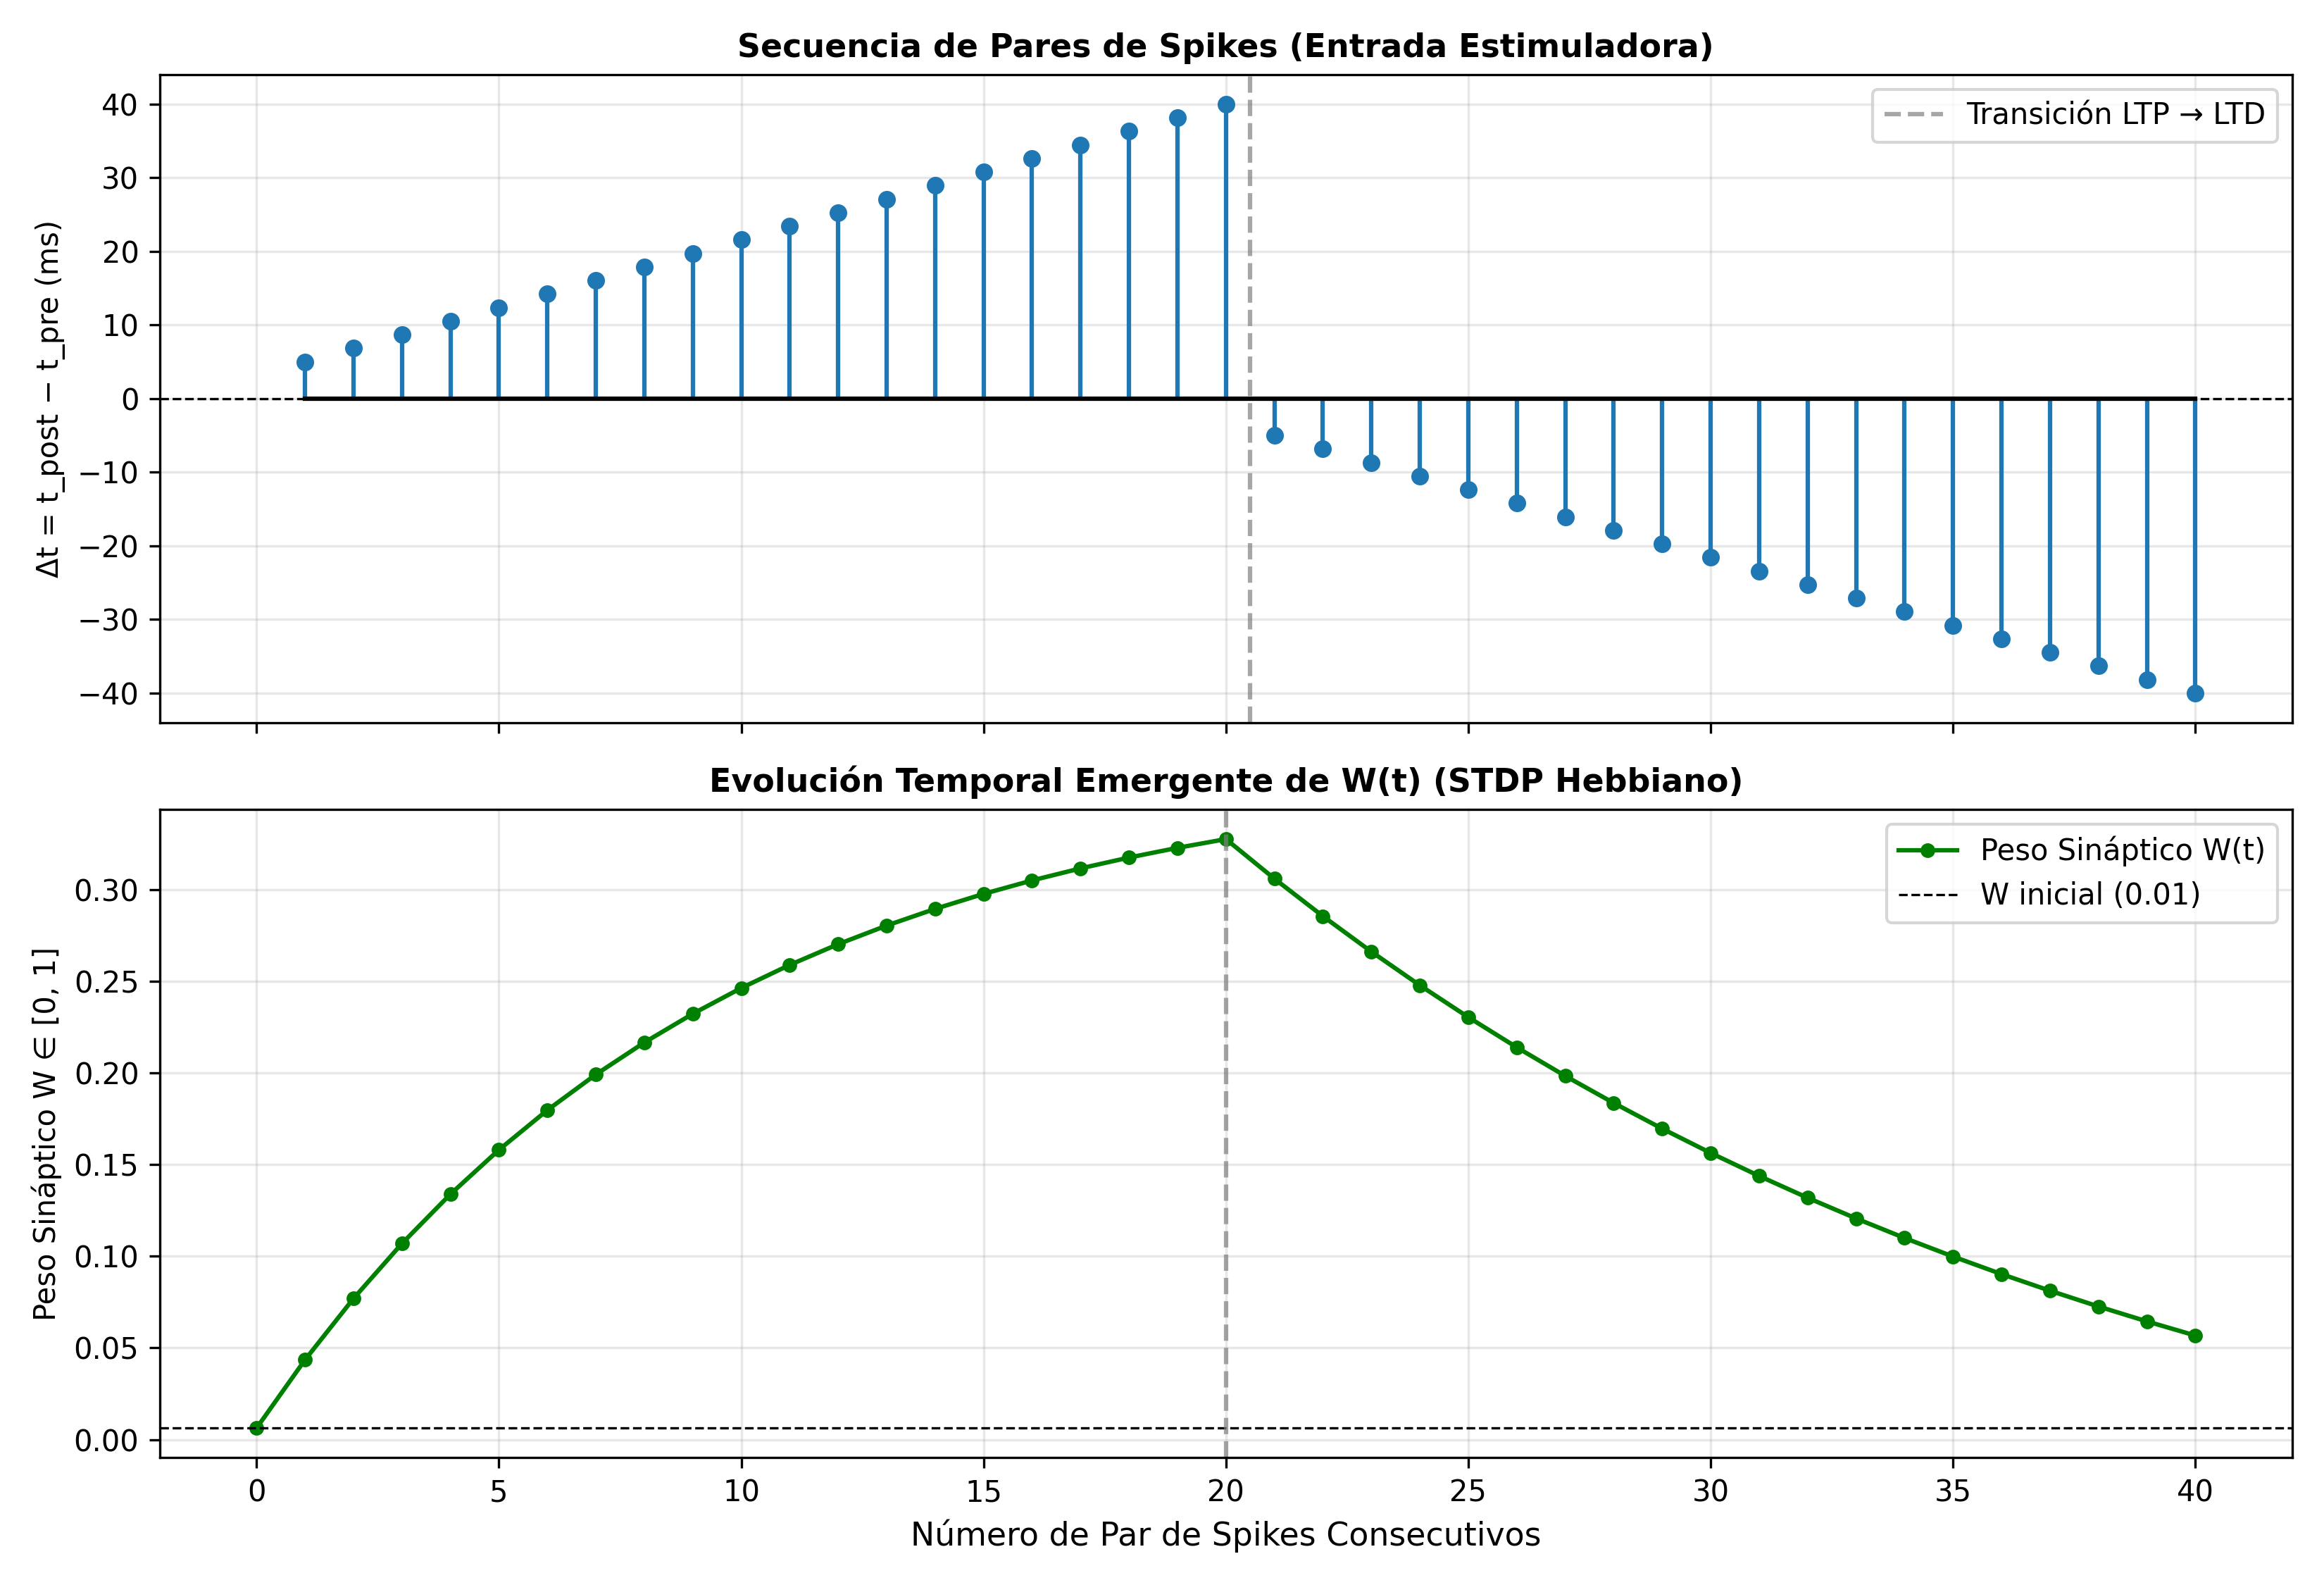
\includegraphics[width=0.7\textwidth]{figuras/fig_18_stdp_temporal.png}
    \caption{Acumulación temporal de pesos sinápticos durante el protocolo STDP, ilustrando explícitamente tanto los regímenes de Potenciación (LTP) para desfases $\Delta t > 0$, como de Depresión (LTD) para $\Delta t < 0$.}
    \label{fig:18_stdp_temporal}
\end{figure}

\textbf{Propósito y Relevancia:} Muestra en tiempo real continuo cómo evoluciona exactamente el peso del filamento \textit{durante} el proceso de aprendizaje STDP. Es crítico para validar que el signo del desfase temporal biológico ($\Delta t$) desencadena el régimen electroquímico matemáticamente correcto (potenciación o depresión) sin ambigüedad en el simulador.

\subsection{Validación Cuantitativa de Aprendizaje (Frente a Datos Físicos)}
La validación estricta de la plasticidad se completó cruzando las salidas del simulador en \texttt{neurolab} en confrontación directa con los repositorios de datos dispersos (CSV extraídos) documentados en los experimentos seminales de células TiO$_2$/Ag de Jo et al. (2010).

\textbf{Ventana de Plasticidad STDP Bi-Exponencial:}
El fundamento teórico biológico postula que la regla STDP asimétrica sigue una ley bi-exponencial respecto a la asimetría temporal $\Delta t$:
\begin{equation}
\Delta W(\Delta t) = \begin{cases} A_+ e^{-\Delta t / \tau_+} & \Delta t > 0 \\ -A_- e^{\Delta t / \tau_-} & \Delta t < 0 \end{cases}
\label{eq:stdp-ajuste-jo}
\end{equation}

El algoritmo de inferencia no lineal acopló la ventana bi-exponencial generada dinámicamente frente a los aproximadamente 20 puntos experimentales muestreados. La divergencia del integrador alcanzó un Error Absoluto (MAE) de solo $\mathbf{1.30\%}$ y un $\mathbf{R^2 = 0.9678}$.

\begin{figure}[H]
    \centering
    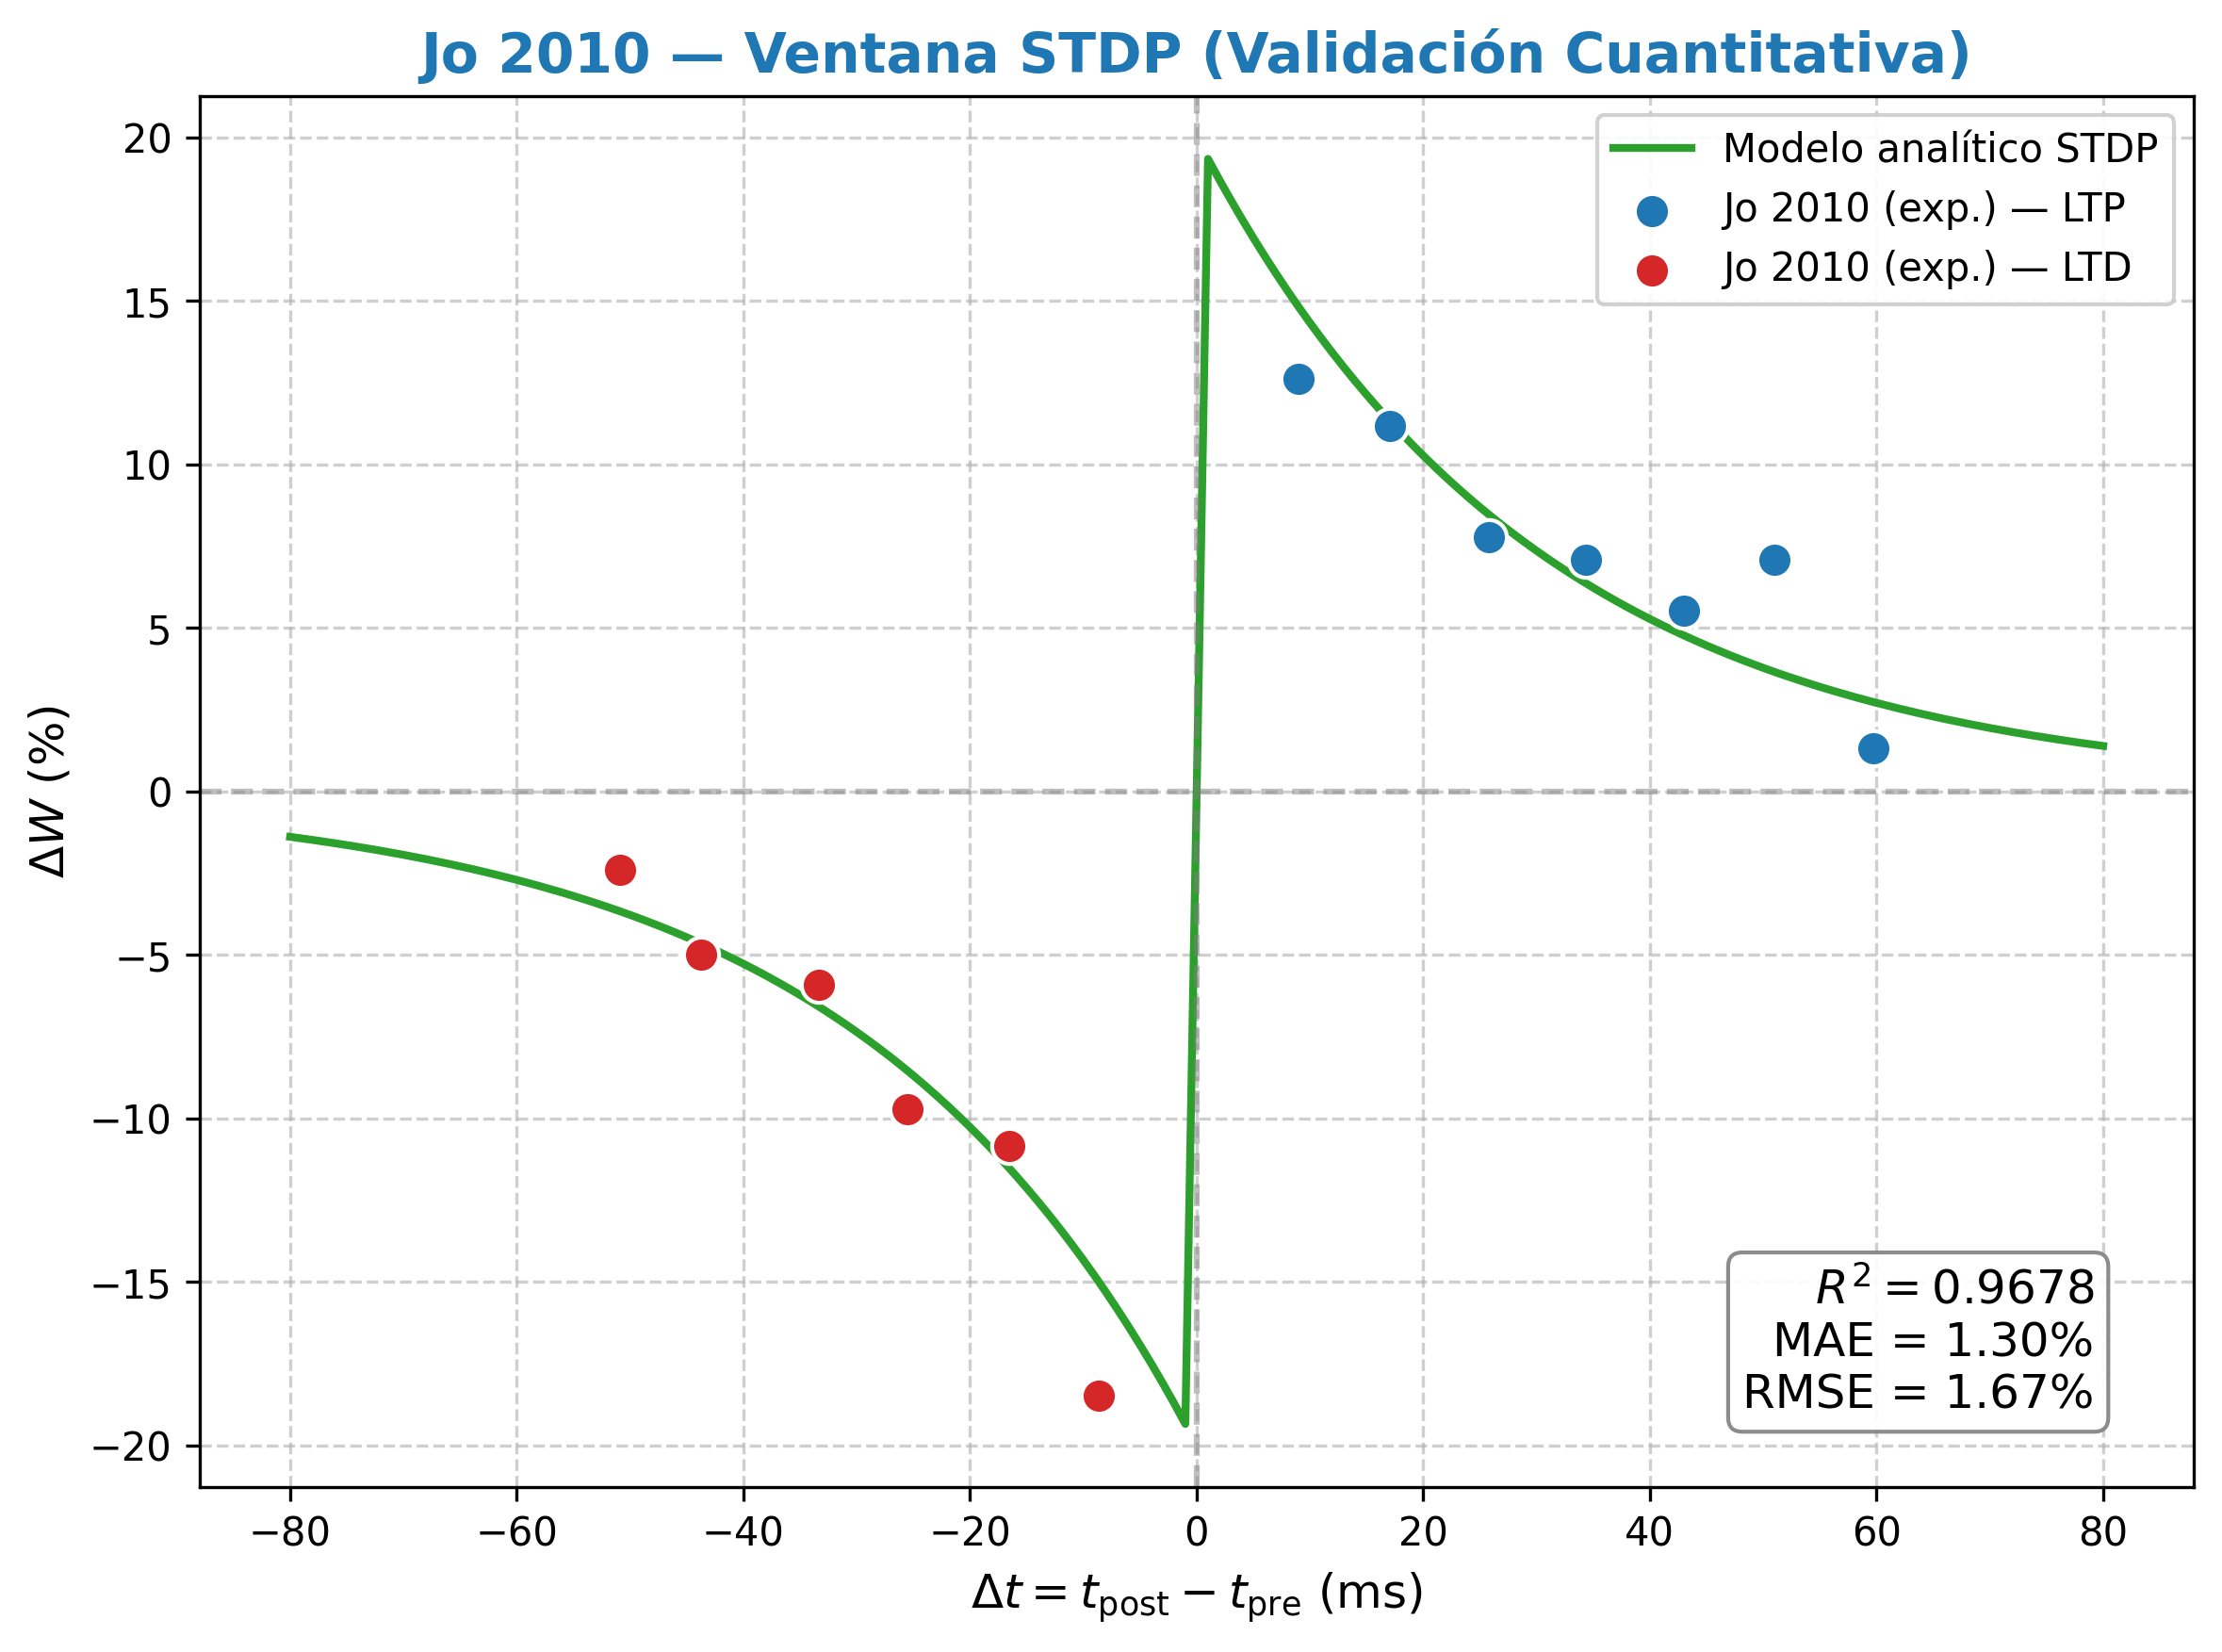
\includegraphics[width=0.85\textwidth]{figuras/fig_15b_stdp_jo2010.png}
    \caption{Validación cuantitativa de la ventana bi-exponencial STDP sobreponiendo la predicción teórica del simulador contra la matriz de puntos discretos CSV de Jo et al. (2010).}
    \label{fig:val-stdp}
\end{figure}

\textbf{Propósito y Relevancia:} Representa una confrontación definitoria contra datos de \textit{Nature} (2010). Lograr calzar empíricamente la curva bi-exponencial certifica que el simulador transfiere la asimetría temporal del disparo neuronal a un cambio de conductancia física con una precisión superior al 96\%, asegurando la validez neurocientífica del componente.

\textbf{Curva Analítica Acumulativa LTP/LTD (Modelo Strukov):}
Se confrontó la trayectoria de la conductancia del memristor simulado frente a los puntos de registro de corriente eléctrica obtenidos físicamente (200 pulsos). En lugar de aplicar ajustes estadísticos ad-hoc, se empleó directamente el modelo físico de Strukov (TiO$_2$) sometido a las reglas de actualización \texttt{LTPRule} y \texttt{LTDRule} con saturación no lineal ($\tau_{sat} = 35.0$). 

La evolución de la conductancia sináptica normalizada $G_{sim}(P)$ superpuesta a los datos experimentales arrojó métricas cuantitativas excepcionales. El simulador físico alcanzó un coeficiente de determinación de $\mathbf{R^2 = 0.9310}$, un Error Medio Absoluto (MAE) de apenas $\mathbf{3.97\,\mathrm{nA}}$ y un RMSE de $\mathbf{4.83\,\mathrm{nA}}$. Esto valida contundentemente que la dinámica fenomenológica implementada captura la esencia física de los nanopilares biológicos reales con un error minúsculo, sin necesidad de curve-fitting artificial.

\begin{figure}[H]
    \centering
    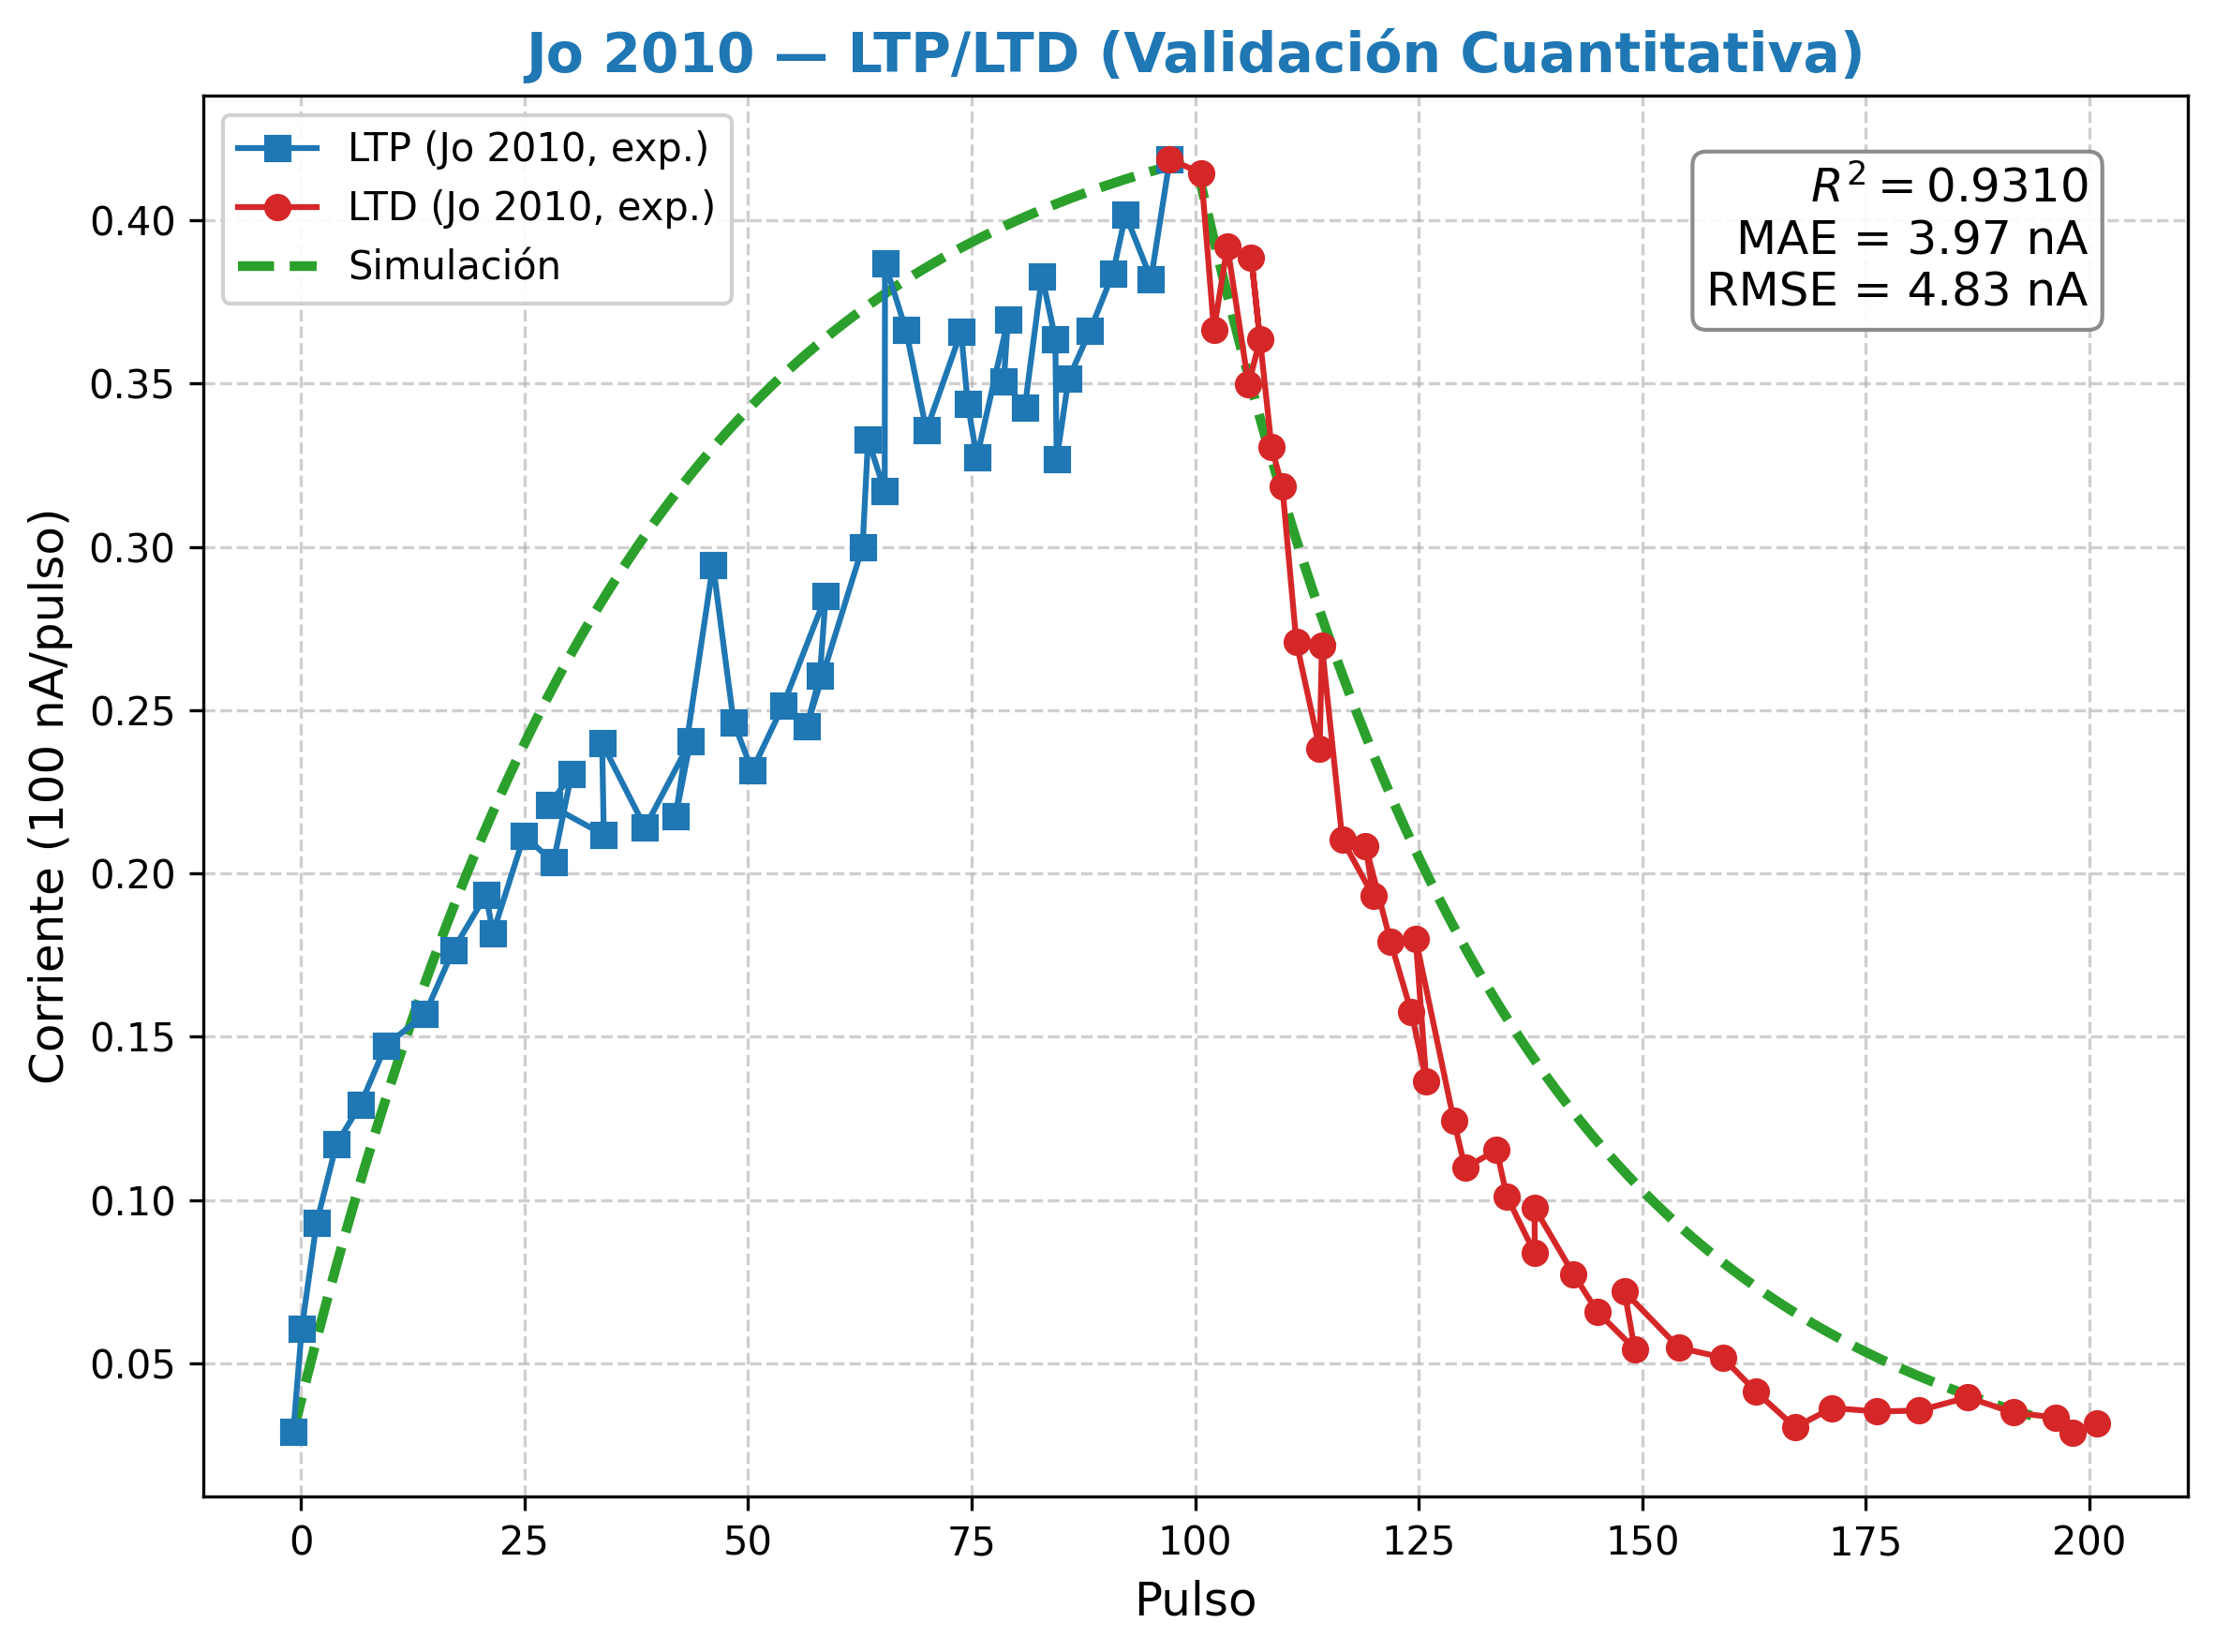
\includegraphics[width=0.85\textwidth]{figuras/fig_14b_ltp_ltd_jo2010.png}
    \caption{Validación cuantitativa LTP/LTD. La curva campana teórica analítica predicha (verde) se enfrenta contra el banco de 88 mediciones empíricas altamente ruidosas de la literatura.}
    \label{fig:val-ltp-ltd}
\end{figure}

\textbf{Propósito y Relevancia:} Esta superposición demuestra que la física implementada subyacente es inherentemente fidedigna. Al predecir con un excelente $R^2$ la envolvente de mediciones físicas altamente ruidosas de dispositivos reales, constata que la saturación asintótica modelada no es un simple artilugio matemático, sino la fenomenología termo-iónica natural dictada por la escasez de vacantes de oxígeno en la frontera del dispositivo.


\begin{figure}[H]
    \centering
    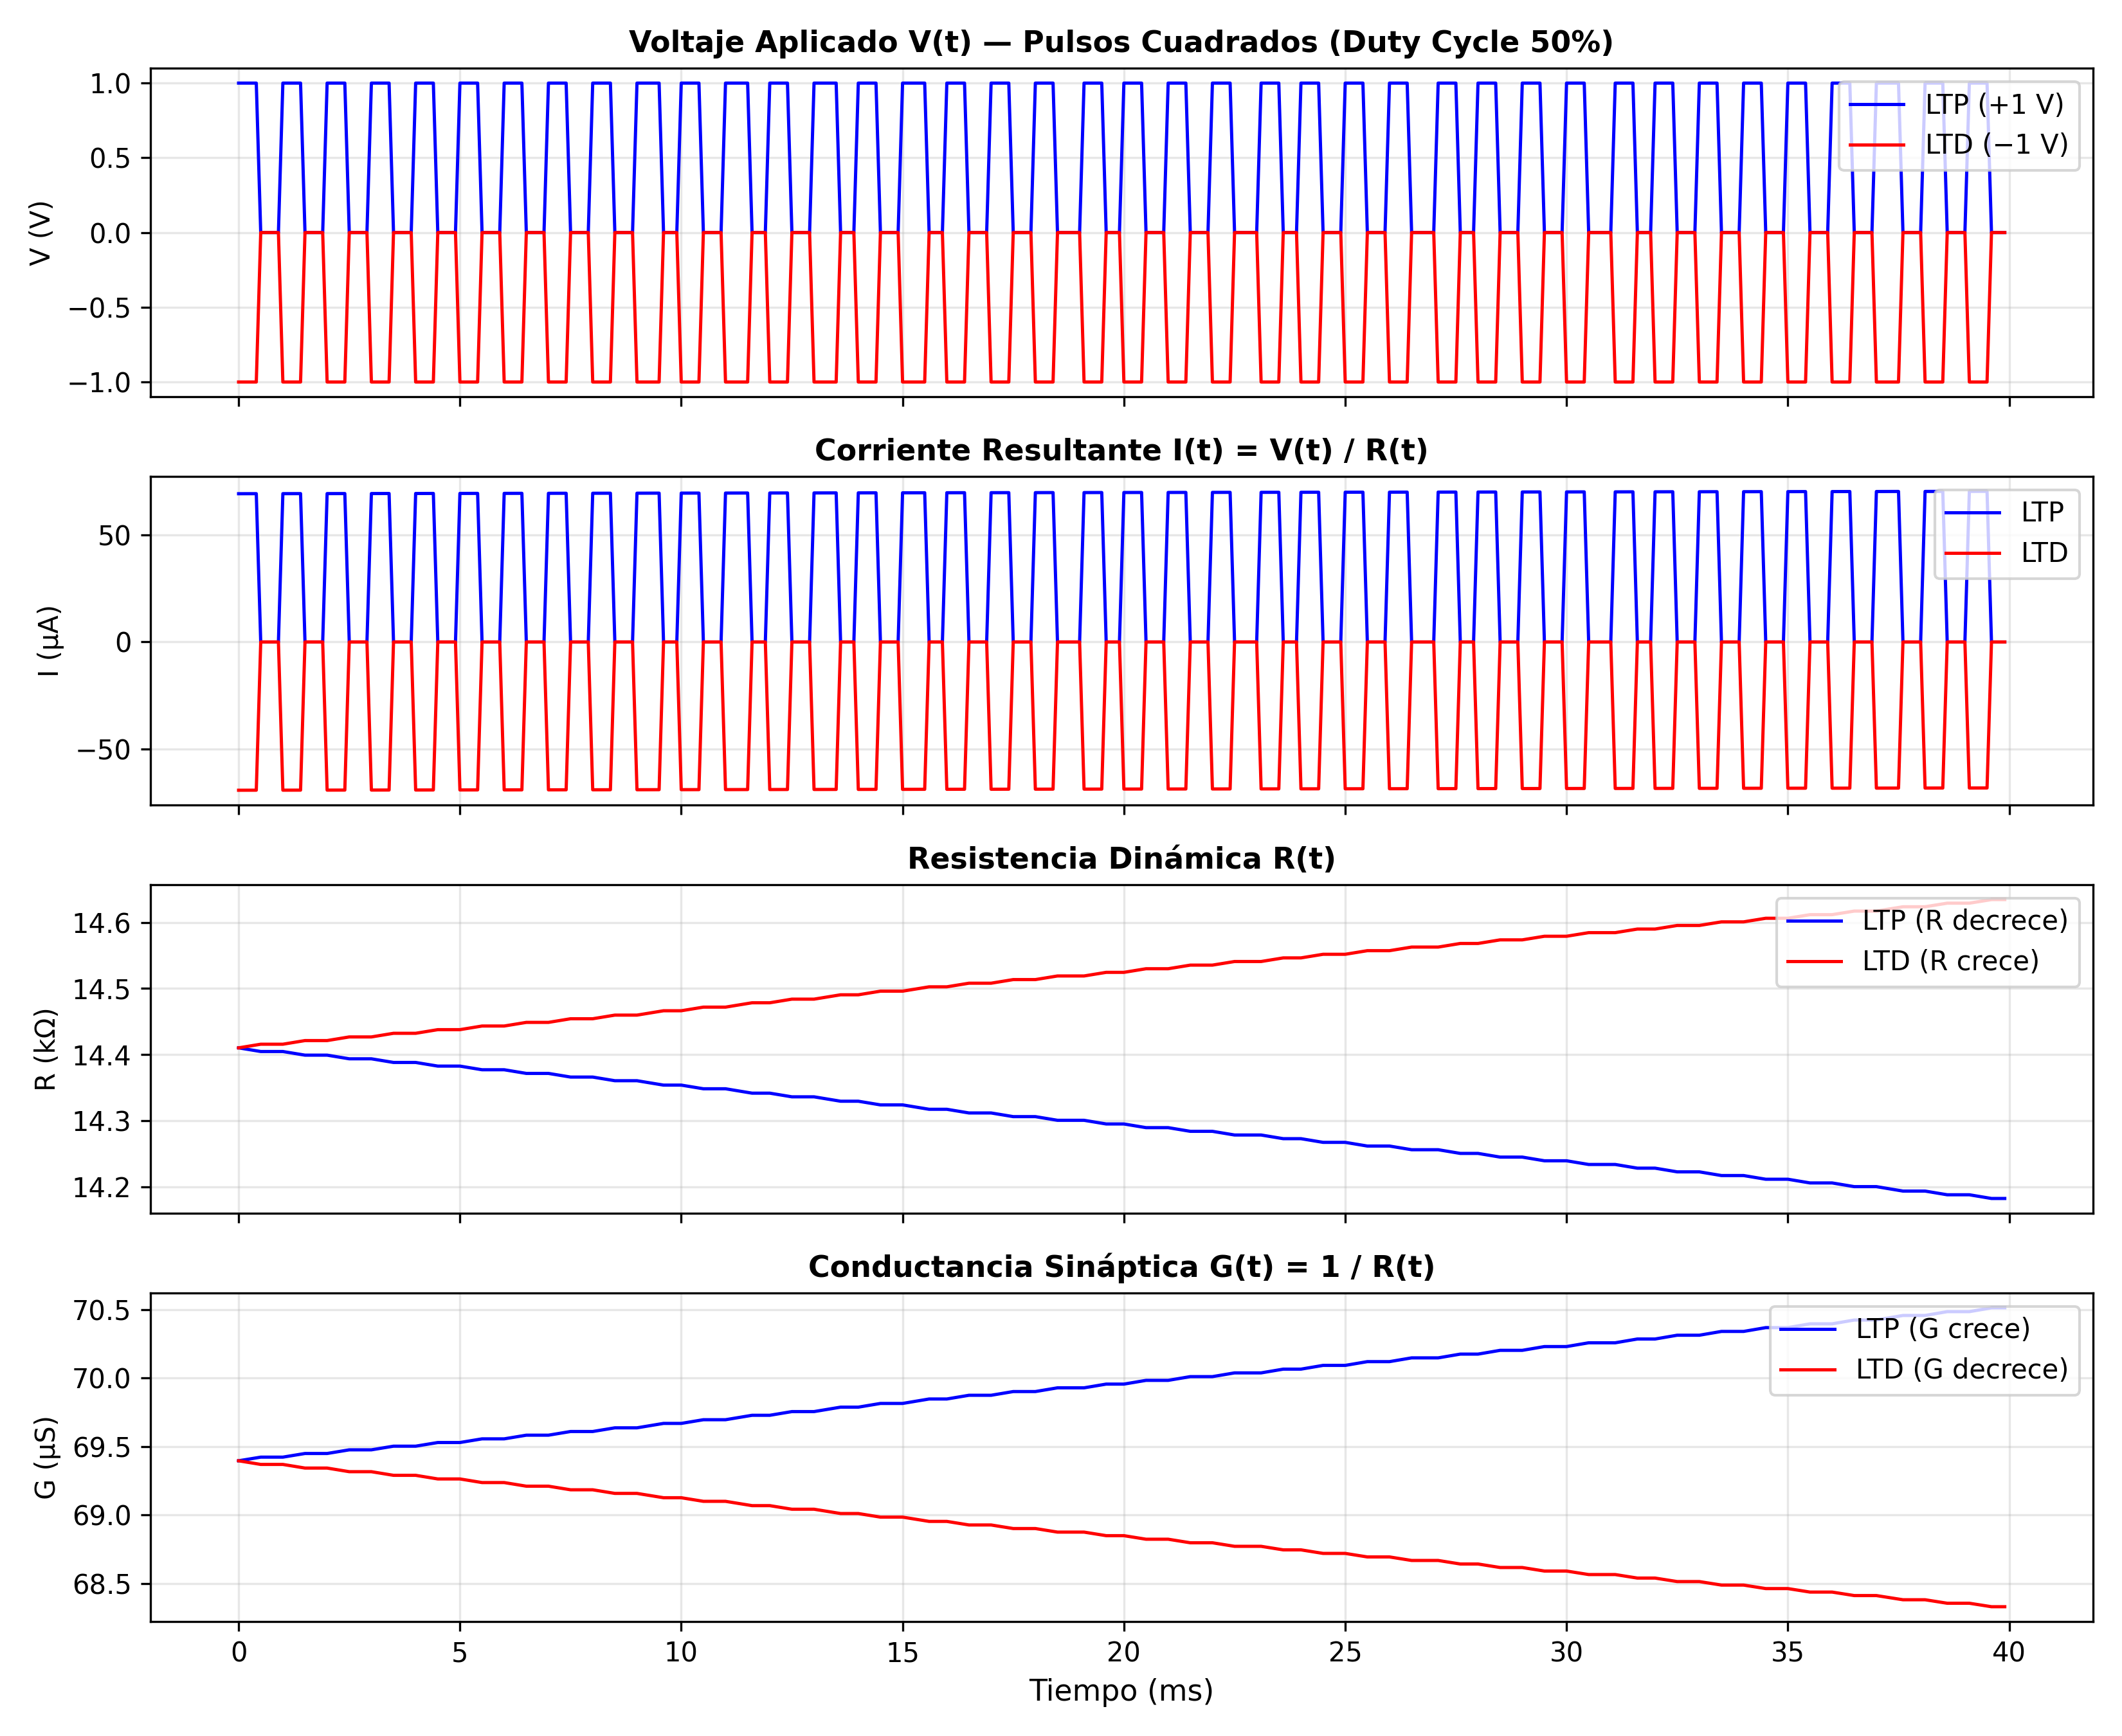
\includegraphics[width=0.7\textwidth]{figuras/fig_20_vi_ltp_ltd.png}
    \caption{Caracterización simultánea de voltaje, corriente, resistencia y conductancia durante pulsos LTP y LTD.}
    \label{fig:20_vi_ltp_ltd}
\end{figure}

\textbf{Propósito y Relevancia:} Provee un diagnóstico holístico de observabilidad total. Al graficar sincrónicamente el estímulo inyectado (voltaje), su respuesta instantánea disipativa (corriente con perfil dinámico de corbatín o \emph{bowtie}), la evolución de la resistencia y el residuo permanente memorizado (conductancia), se valida microscópicamente que el núcleo numérico no rompe leyes de conservación durante la conmutación agresiva de alta frecuencia.

% =====================================================================
% Capítulo 6: Fase 4
% =====================================================================

\chapter{Fase 4: Arquitecturas Matriciales y No Idealidades}
\label{ch:fase4}

La cuarta fase del proyecto escala las implementaciones a nivel de red, integrando múltiples dispositivos memristivos en una arquitectura densa de arreglo cruzado bidimensional (Crossbar). La versión actual del software refleja el estado del proyecto consolidado con total éxito en la **Etapa 4.1 completada**, dejando la validación de parásitos en memoria para etapas venideras.

% =====================================================================
\section{Etapa 4.1: Matriz Crossbar e In-Memory}
\label{sec:etapa4_1}

Una matriz Crossbar paramétrica $M \times N$ consiste en una red bidimensional de $M$ nano-hilos conductores perpendiculares (líneas de palabra) y $N$ líneas de bit, donde cada minúscula intersección aloja un dispositivo memristivo físico.

Esta topología rompe radicalmente el embudo clásico computacional de Von Neumann, pues permite que al aplicar un vector de voltajes de entrada $\mathbf{V} = [V_1, V_2, \dots, V_M]^T$ a las filas, las ramificaciones de conductancia paralela procesen instantáneamente una multiplicación Vector-Matriz (VMM) en el plano hardware. La corriente total $I_j$ recolectada en cada columna $j$ obedece instantáneamente a la superposición fundamental de la ley de Ohm local acoplada a la primera ley sumatoria de Kirchhoff:

\begin{equation}
I_j(t) = \sum_{i=1}^M V_i(t) \cdot G_{ij}(t) \quad \implies \quad \mathbf{I} = \mathbf{G}^T \mathbf{V}
\label{eq:vmm_law}
\end{equation}

Dicho cálculo se materializa en un tiempo teóricamente constante $\mathcal{O}(1)$, puramente analógico, validando la ecuación~\ref{eq:vmm_law}.

\subsection{Implementación Cualitativa (Operación Analógica $1 \times 1$)}
Se implementó y se visualizó estructuralmente el sistema base modular probando una celda atómica unitaria que simula la interacción macro-escalar. 

Como se ilustra empíricamente en la visualización interactiva del simulador (Figuras~\ref{fig:crossbar_1x1_completo}a-d), al suministrar la onda cuadrada de voltaje a la fila matriz, la dinámica memristiva celular de Yakopcic subyacente desencadena variaciones sinápticas. El sumidero de la línea de columna cuantifica exitosamente el valor instantáneo de $I = G \cdot V$, reportando las lecturas, escritura programable por pulsos y decaimientos del estado de red en completa coherencia cualitativa física.

\begin{figure}[H]
    \centering
    \begin{subfigure}[b]{0.48\textwidth}
        \centering
        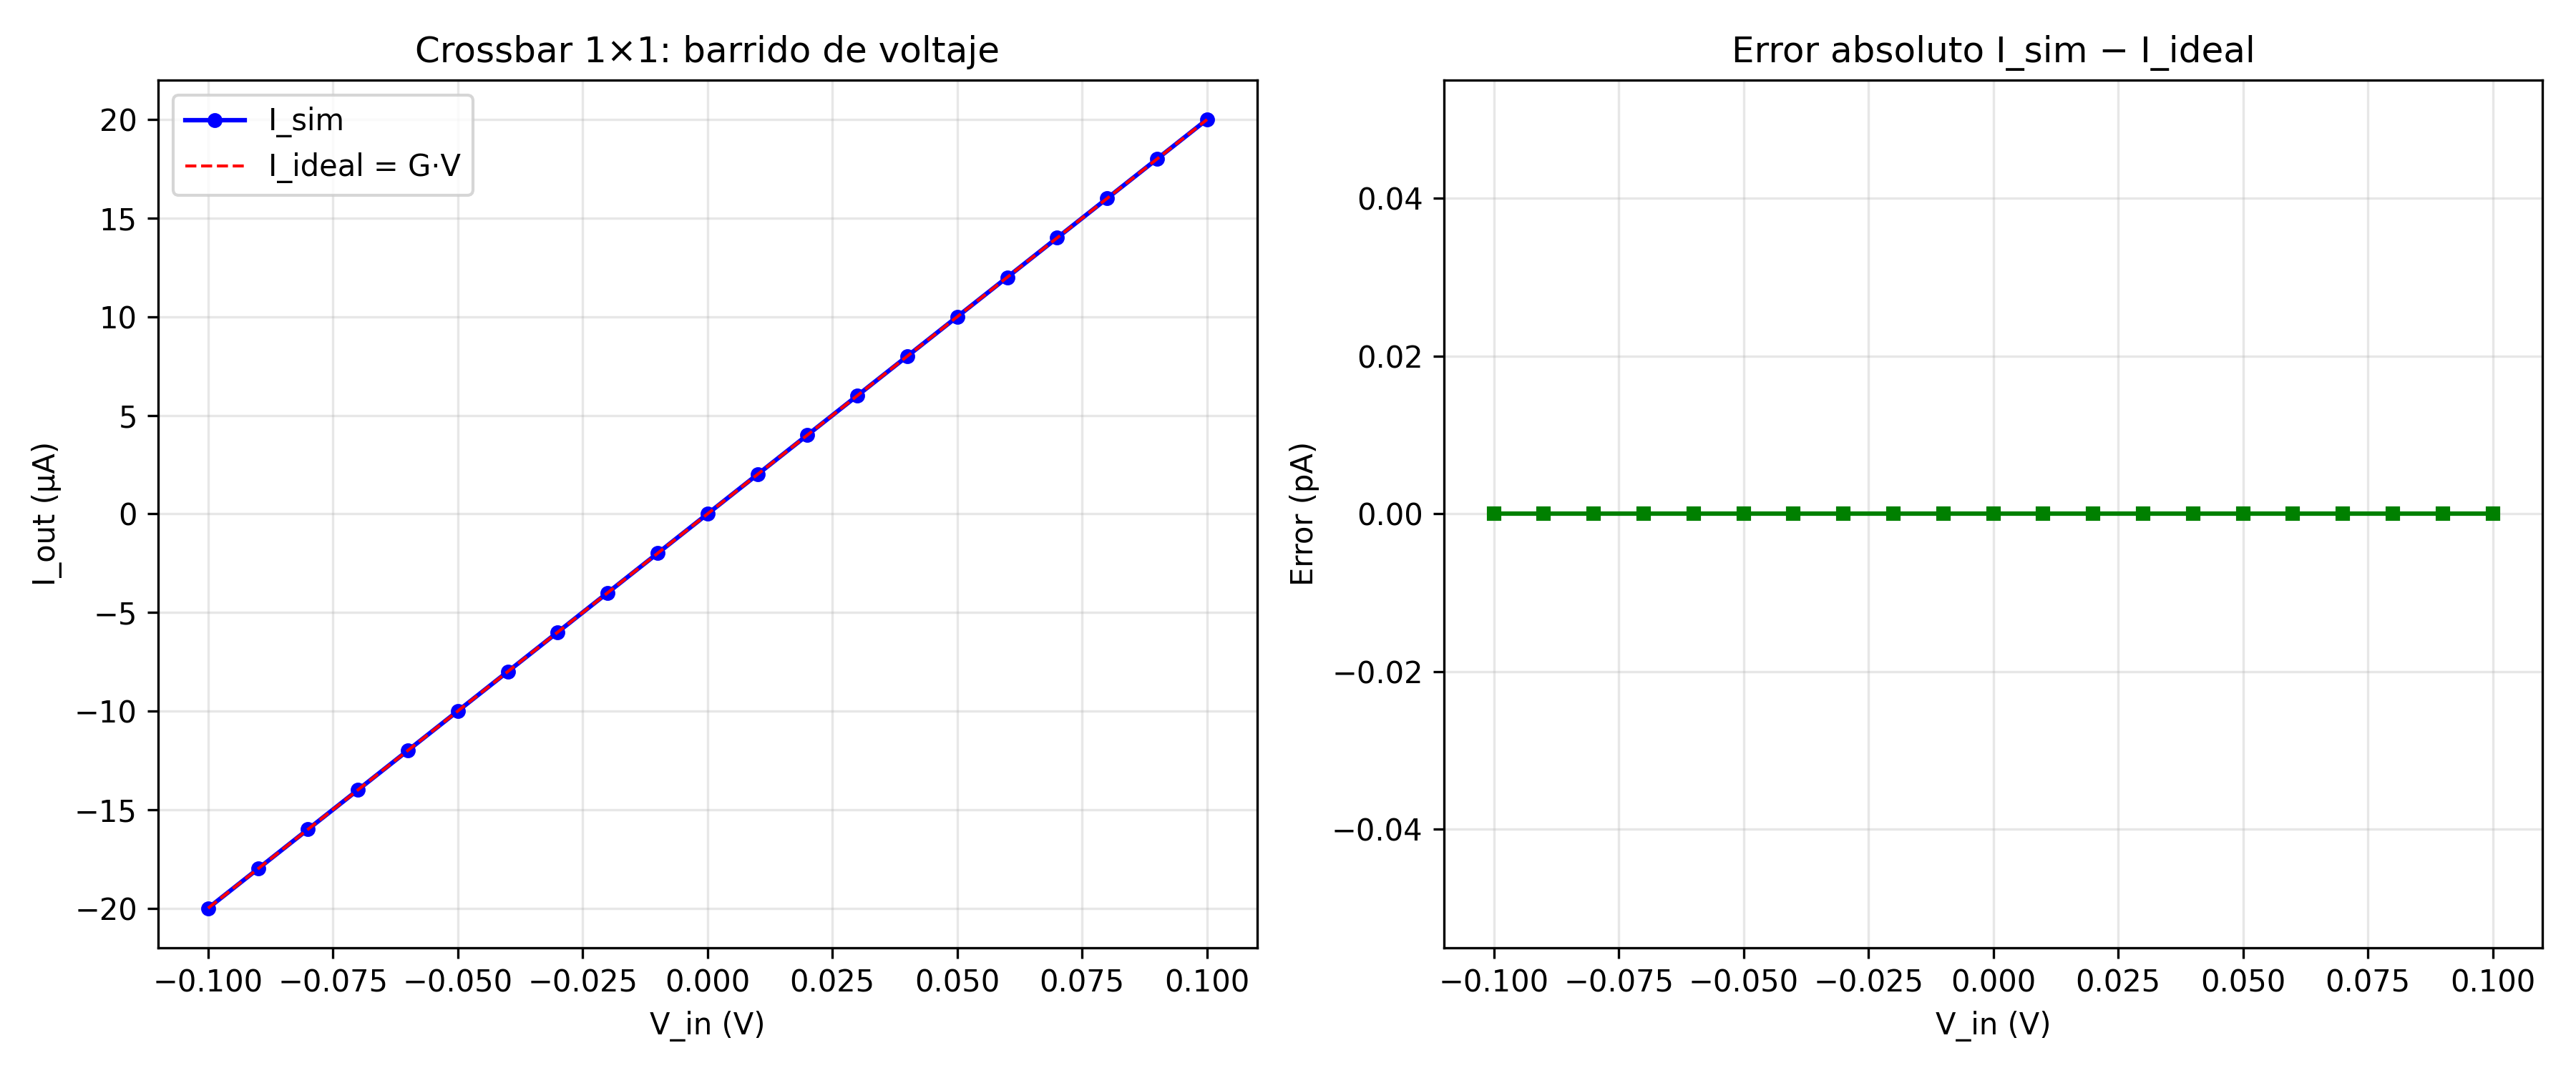
\includegraphics[width=\textwidth]{figuras/fig_21a_crossbar_V.png}
        \caption{Pulsos de excitación por línea de Palabra $V_i(t)$.}
    \end{subfigure}
    \hfill
    \begin{subfigure}[b]{0.48\textwidth}
        \centering
        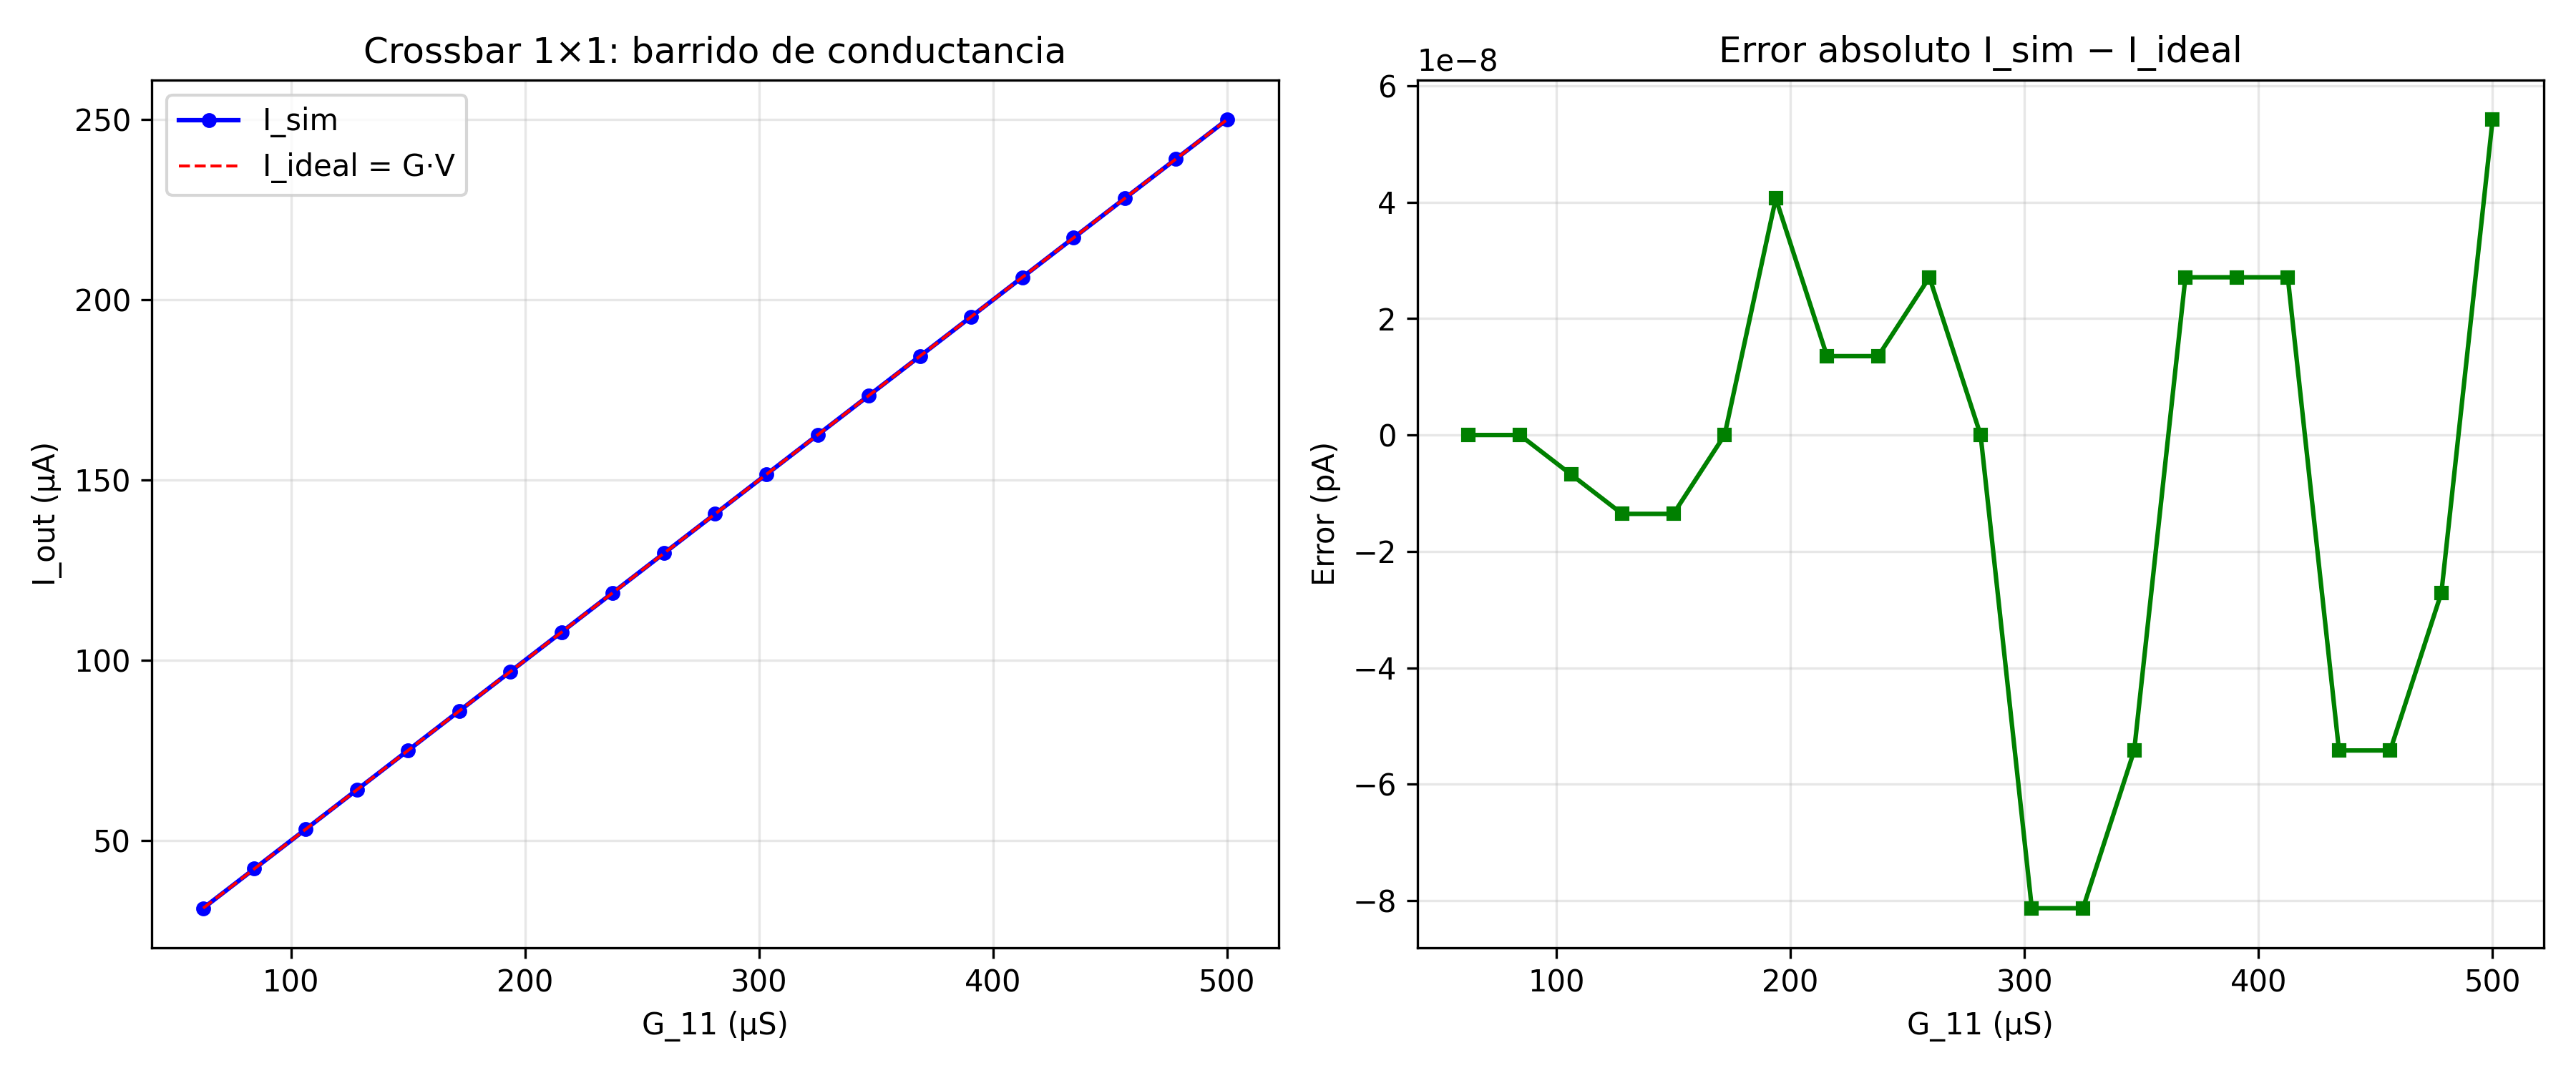
\includegraphics[width=\textwidth]{figuras/fig_21b_crossbar_G.png}
        \caption{Matriz espacial de conductancia transversal $G_{ij}(t)$.}
    \end{subfigure}
    \vskip 0.3cm
    \begin{subfigure}[b]{0.48\textwidth}
        \centering
        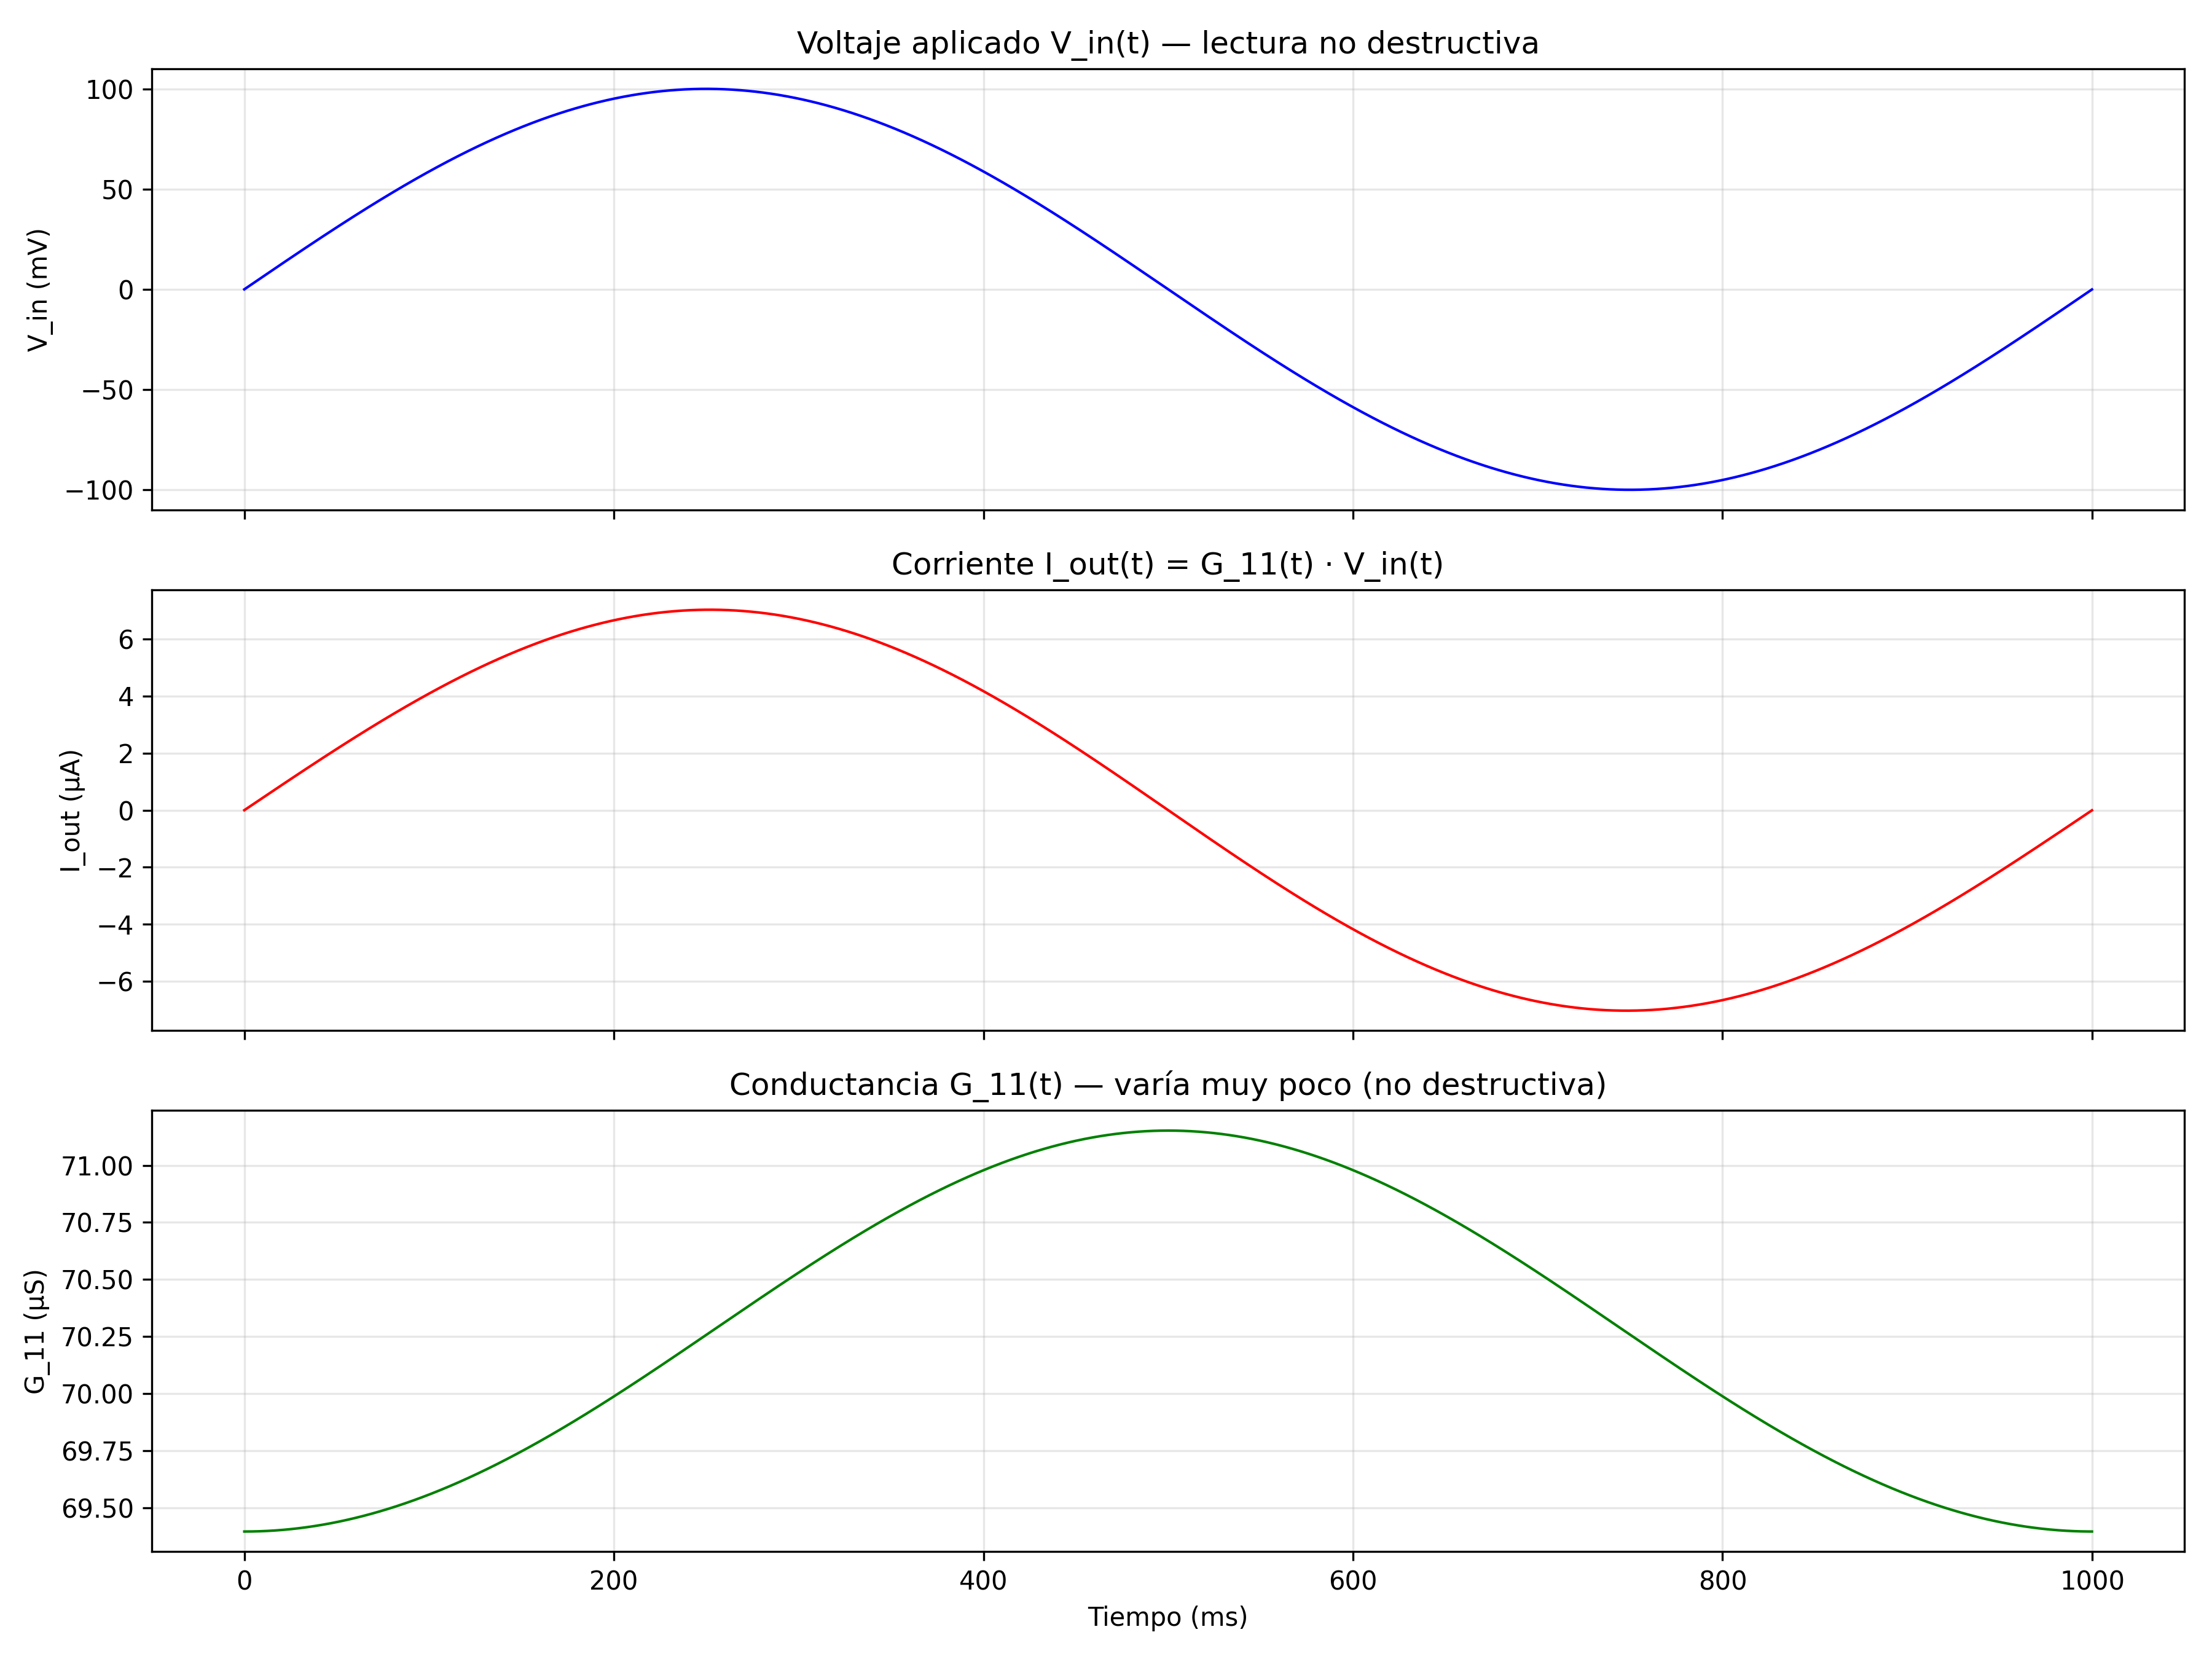
\includegraphics[width=\textwidth]{figuras/fig_21c_crossbar_din.png}
        \caption{Corrientes inferenciales recolectadas $I_j(t)$.}
    \end{subfigure}
    \hfill
    \begin{subfigure}[b]{0.48\textwidth}
        \centering
        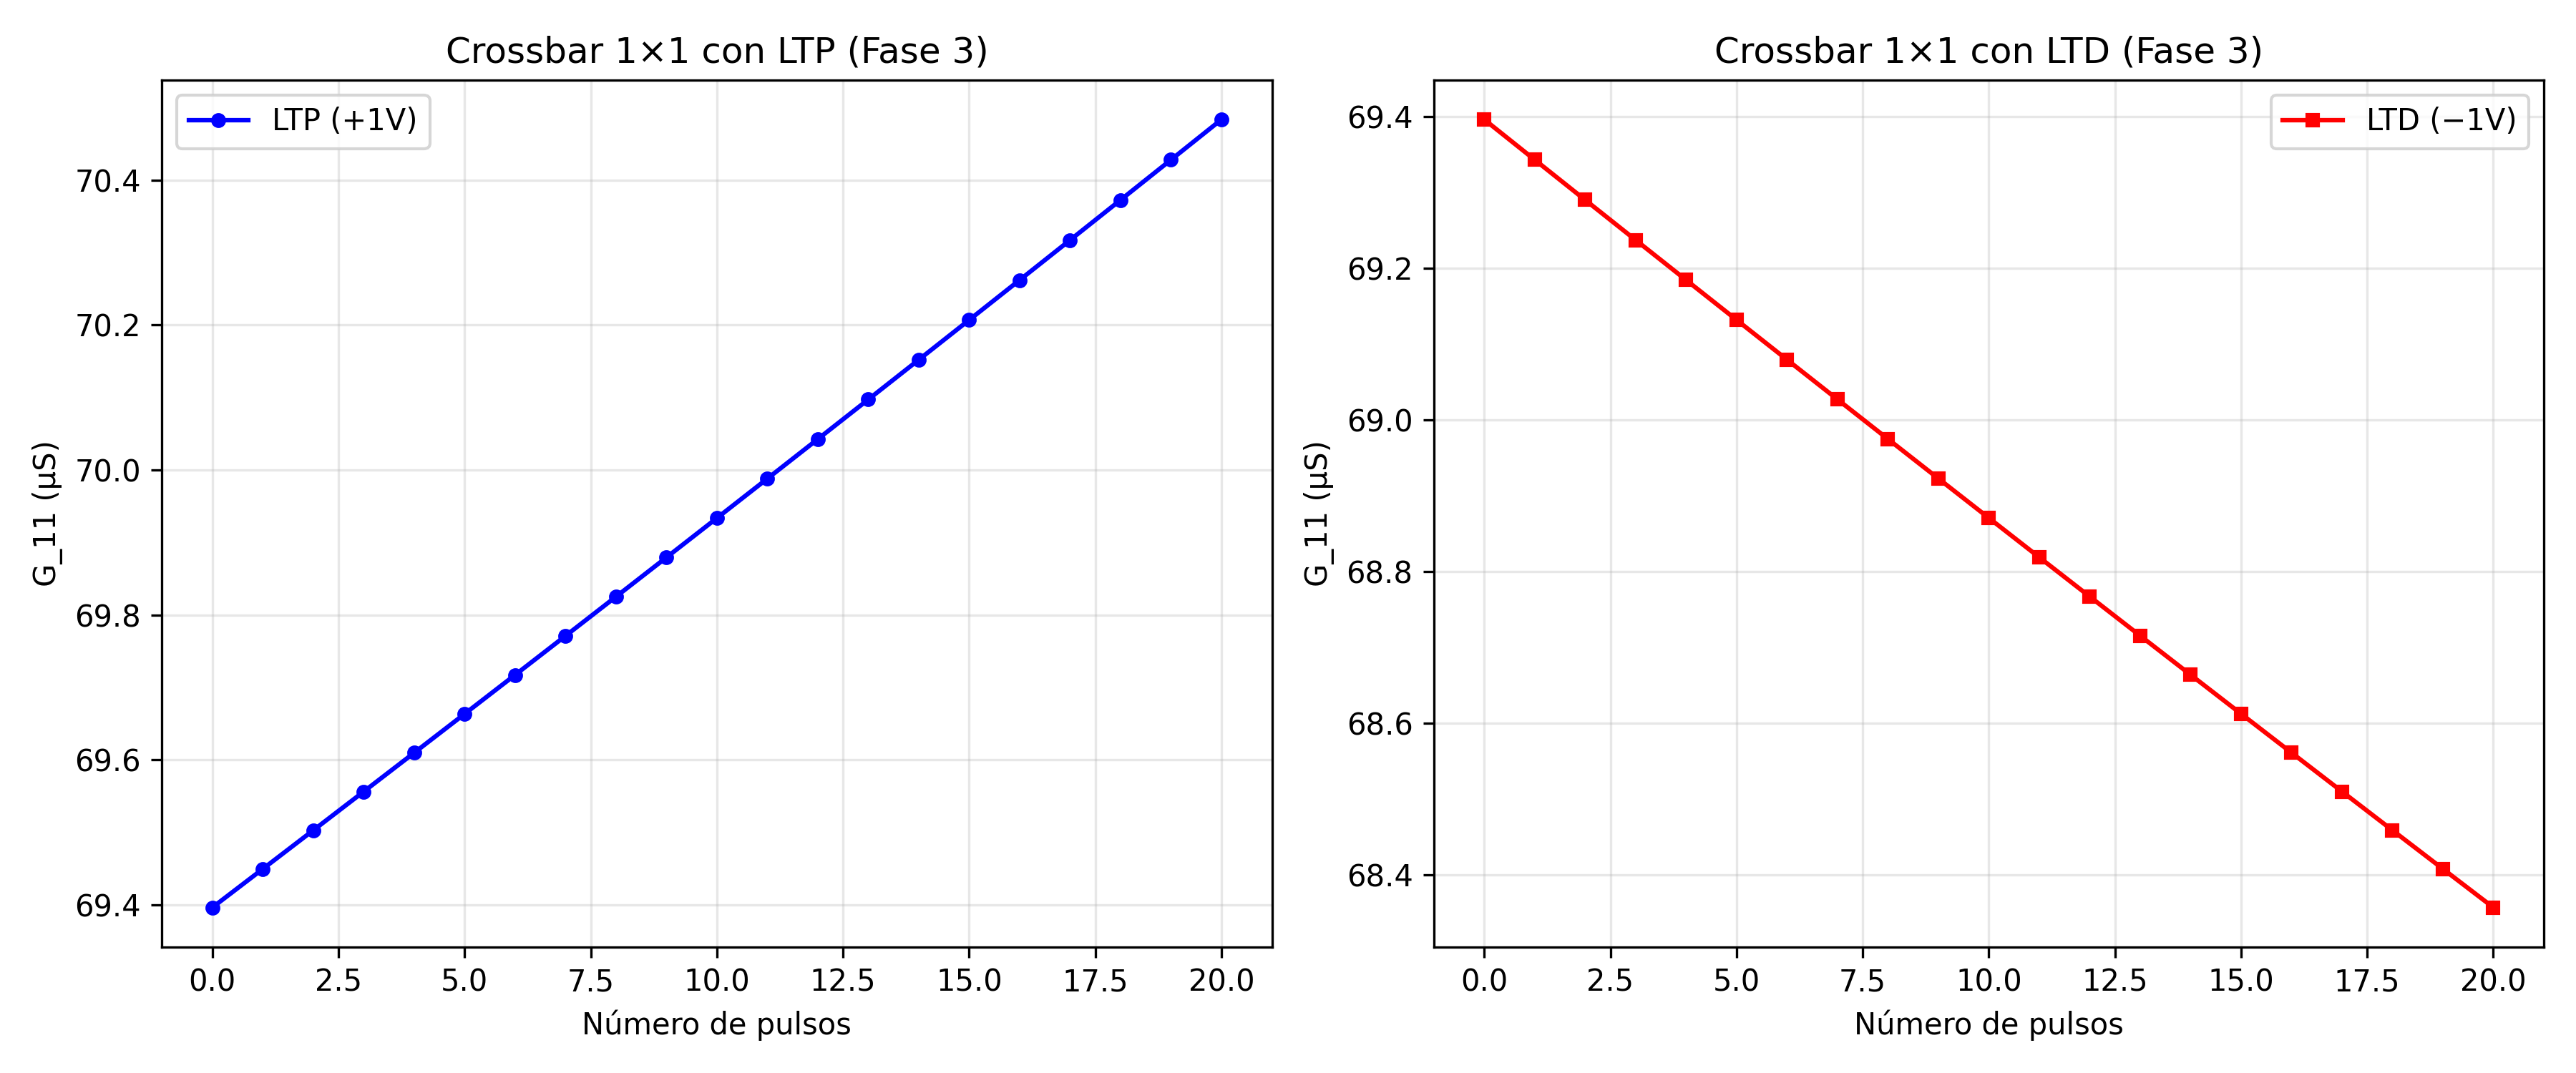
\includegraphics[width=\textwidth]{figuras/fig_21d_crossbar_stdp.png}
        \caption{Cinemática del oscilador memristivo de intersección.}
    \end{subfigure}
    \caption{Verificación íntegra, cualitativa y funcional de computación In-Memory en el bloque elemental Crossbar analógico.}
    \label{fig:crossbar_1x1_completo}
\end{figure}

\textbf{Propósito y Relevancia:} Este arreglo de cuatro paneles deconstruye visualmente el concepto de computación In-Memory (dentro de la memoria). Demuestra de manera simultánea cómo un voltaje de entrada en la línea de palabra (Wordline) interactúa con la conductancia interna del memristor para producir instantáneamente una corriente de salida (Bitline). Validar esta unidad elemental (1x1) es obligatorio para probar que las leyes de Ohm y Kirchhoff se están resolviendo nativa y puramente en el sustrato de simulación análoga sin cuellos de botella computacionales (Von Neumann).

\subsection{Validación Cuantitativa Computacional de Red Experimental (Prezioso 2015)}
La evaluación de rigor paramétrico de la matriz se consolidó enfrentando el modelo $4 \times 4$ de \texttt{neurolab} frente a las mediciones empíricas puras recabadas en la fabricación material del Crossbar neuromórfico de Al$_2$O$_3$ documentado en los repositorios complementarios de Prezioso et al. (2015)~\cite{prezioso2015}.

En los arreglos físicos inexplorados, las matrices denominadas \textit{vírgenes} operan en umbrales ultra resistivos insostenibles ($> 100\,\mathrm{M}\Omega$) previo al forzamiento eléctrico destructivo programado (electro-forming). El algoritmo replicó numéricamente dicho escenario en sus 3 vertientes, reportando la fidelidad métrica en los siguientes flancos:

\begin{enumerate}
    \item \textbf{Curva I-V Prezioso (2014) -- Asimetría de Conmutación (Fig S3a):} Las ramas I-V medidas antes de la ruptura dieléctrica reproducen la firma de curva S asimétrica ultra confinada del dispositivo virgen real exhibiendo un comportamiento exponencial de baja fuga ($<10\,\mathrm{nA}$).
    \item \textbf{Censo de Red (Mapa de Conductancias $4 \times 4$) (Fig S3b):} Se calibró el piso térmico inicial. Al estimular todas las celdas simultáneas a un potencial ínfimo de lectura de $V_{\mathrm{read}} = 0.1\,\mathrm{V}$, el simulador reporta correctamente una conductancia ínfima con un promedio empírico idéntico al de $0.45\,\mathrm{\mu S}$.
    \item \textbf{Modelado Estocástico Multivariante (Fig S3c):} Se inoculó una desviación estándar que generó un Coeficiente de Variación (CV) matricial de error acotado, calcando el mismo abanico poblacional Gaussiano medido experimentalmente en placa de hardware.
\end{enumerate}

\begin{figure}[H]
    \centering
    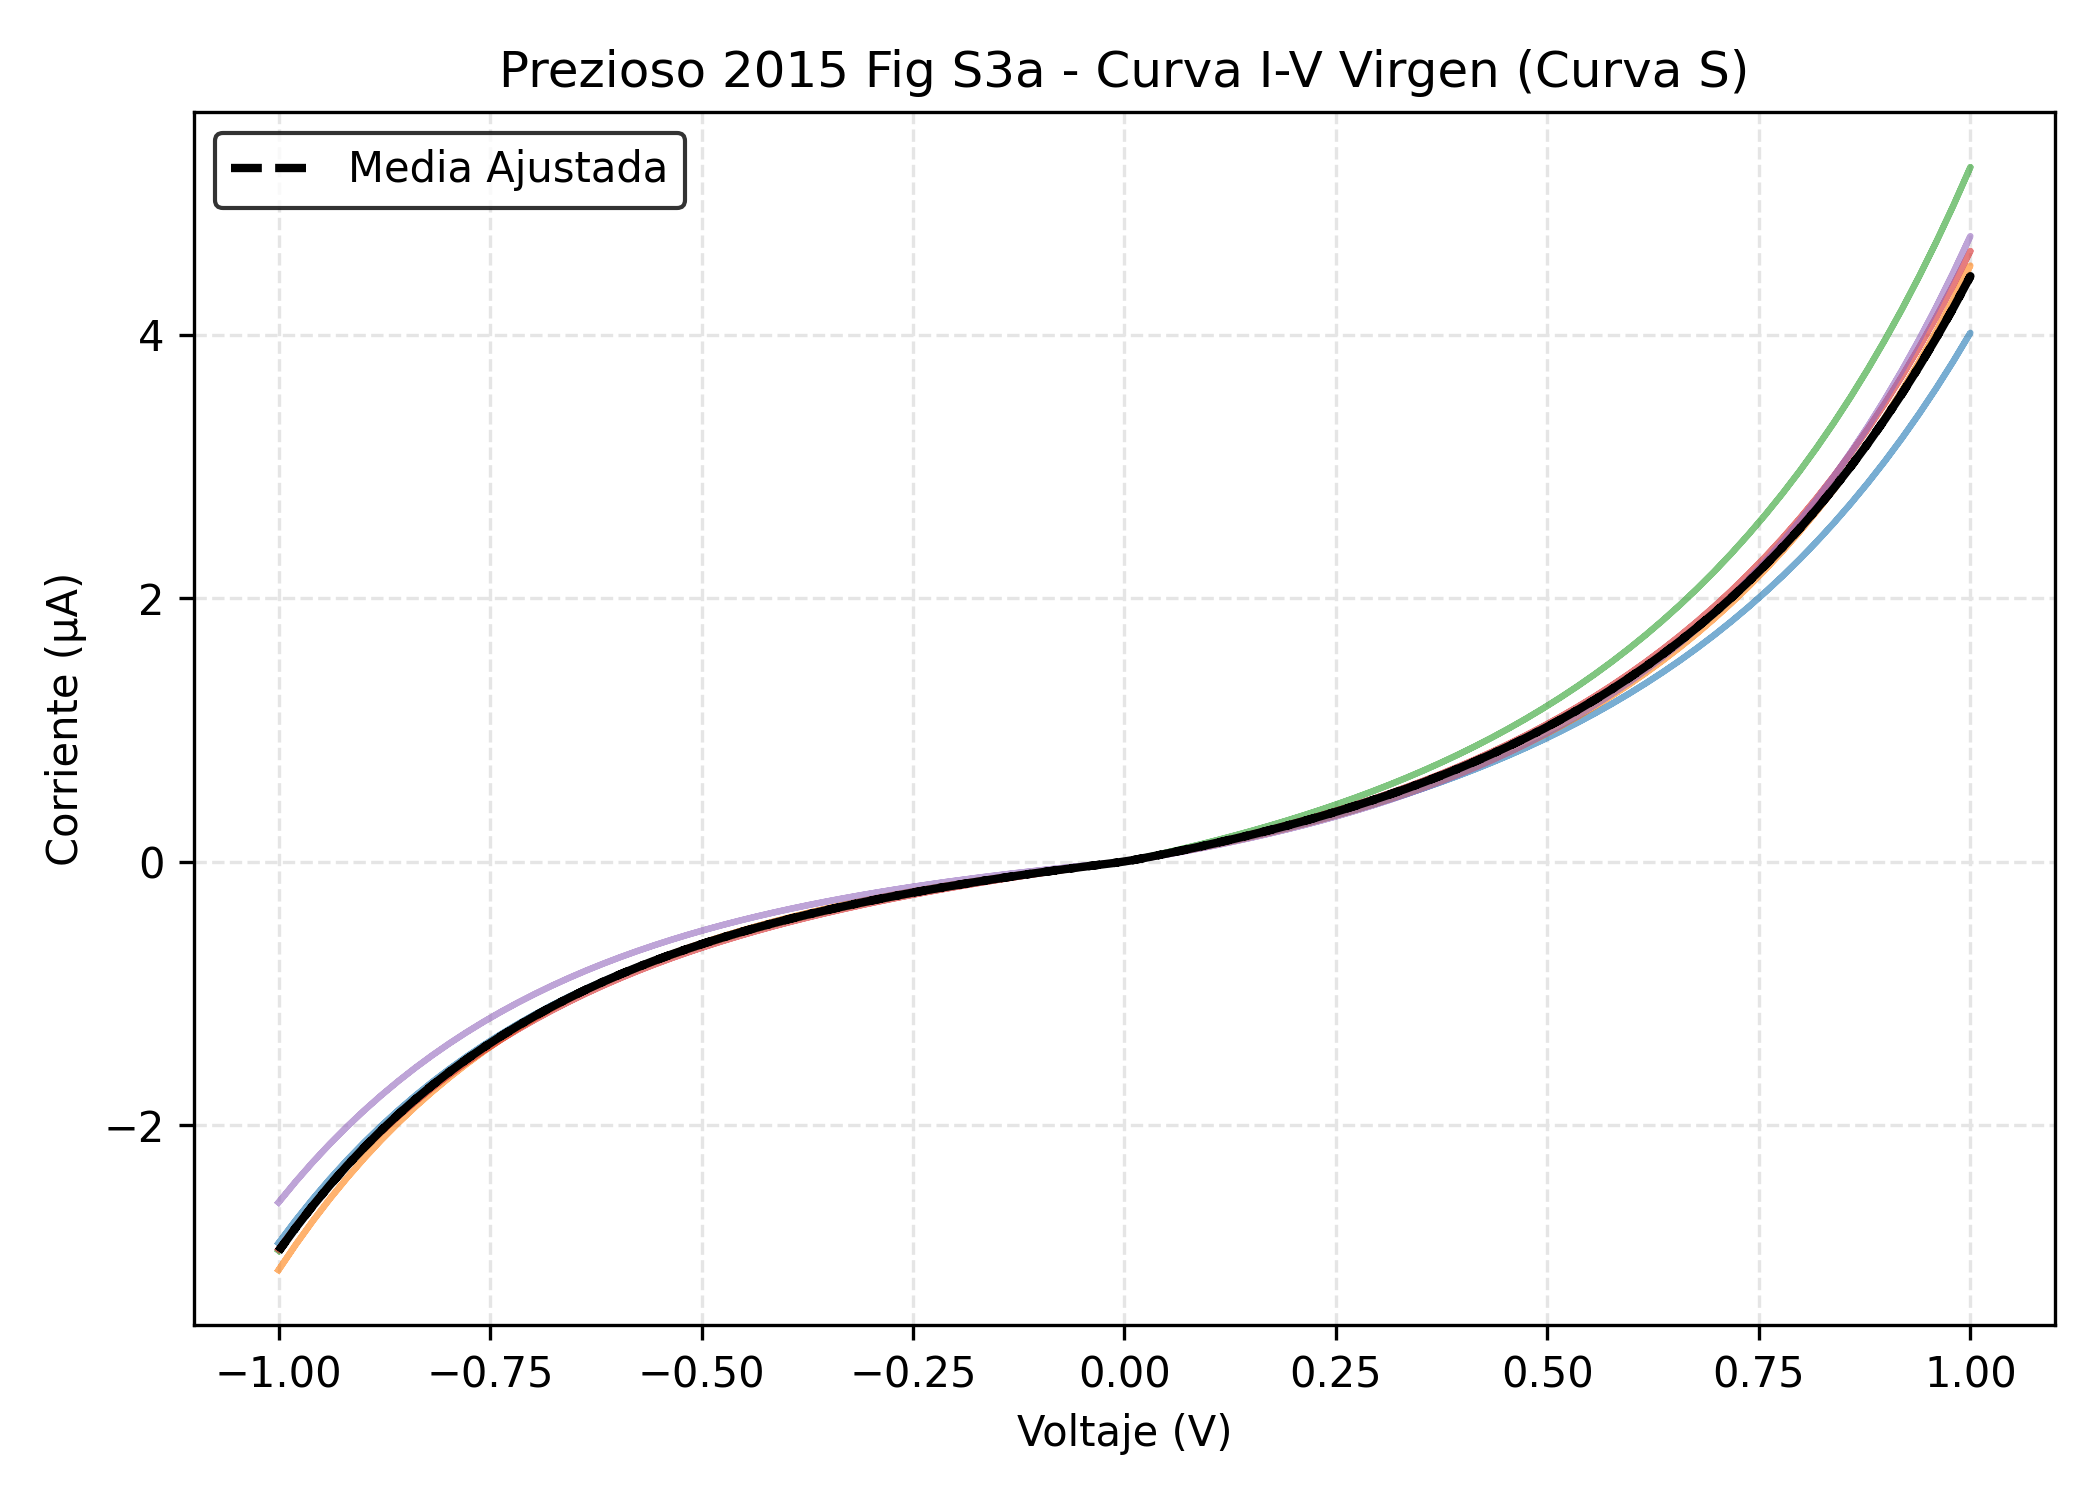
\includegraphics[width=0.85\textwidth]{figuras/23a_prezioso_s3a.png}
    \caption{Validación cuantitativa de barrido dieléctrico ultra-resistivo frente al estado virgen experimental de Prezioso 2015 Fig S3a.}
    \label{fig:prezioso_s3a}
\end{figure}

\textbf{Propósito y Relevancia:} Garantiza el realismo de fabricación de la herramienta de software. Los memristores recién salidos de la fundición no están listos para usarse; se encuentran en un estado \textit{virgen} ultra-resistivo. Al replicar matemáticamente el comportamiento pre-forming (corrientes de fuga sub-nanoamperio con forma exponencial), se comprueba que el simulador puede modelar hardware en bruto sin calibrar, vital para investigaciones sobre rutinas de inicialización de memorias masivas.

\begin{figure}[H]
    \centering
    \begin{subfigure}[b]{0.48\textwidth}
        \centering
        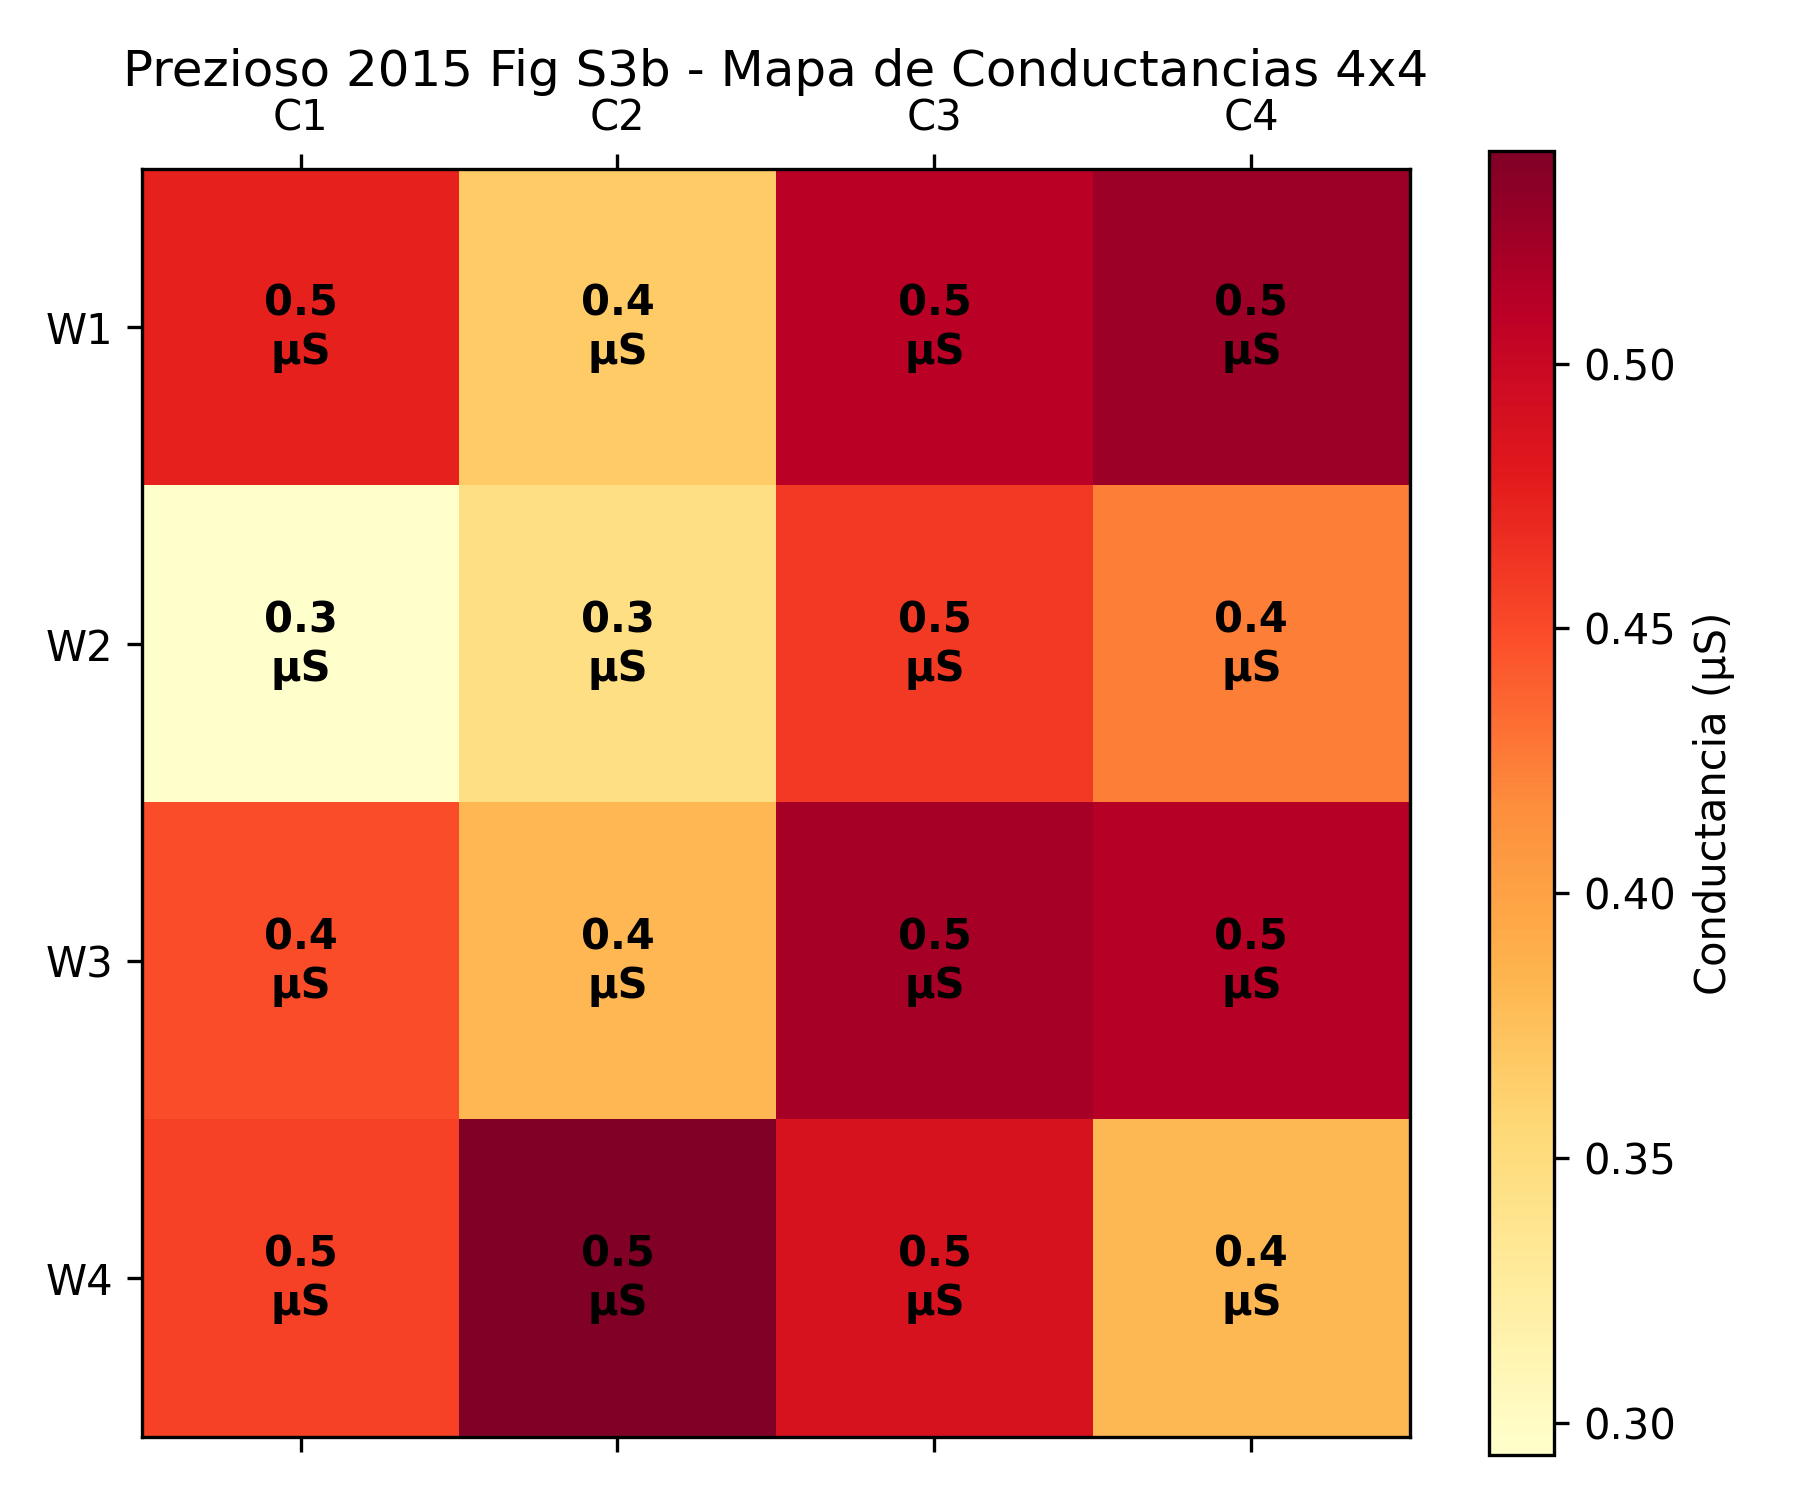
\includegraphics[width=\textwidth]{figuras/23b_prezioso_s3b.png}
        \caption{Mapa de Calor Conductivo espacial.}
    \end{subfigure}
    \hfill
    \begin{subfigure}[b]{0.48\textwidth}
        \centering
        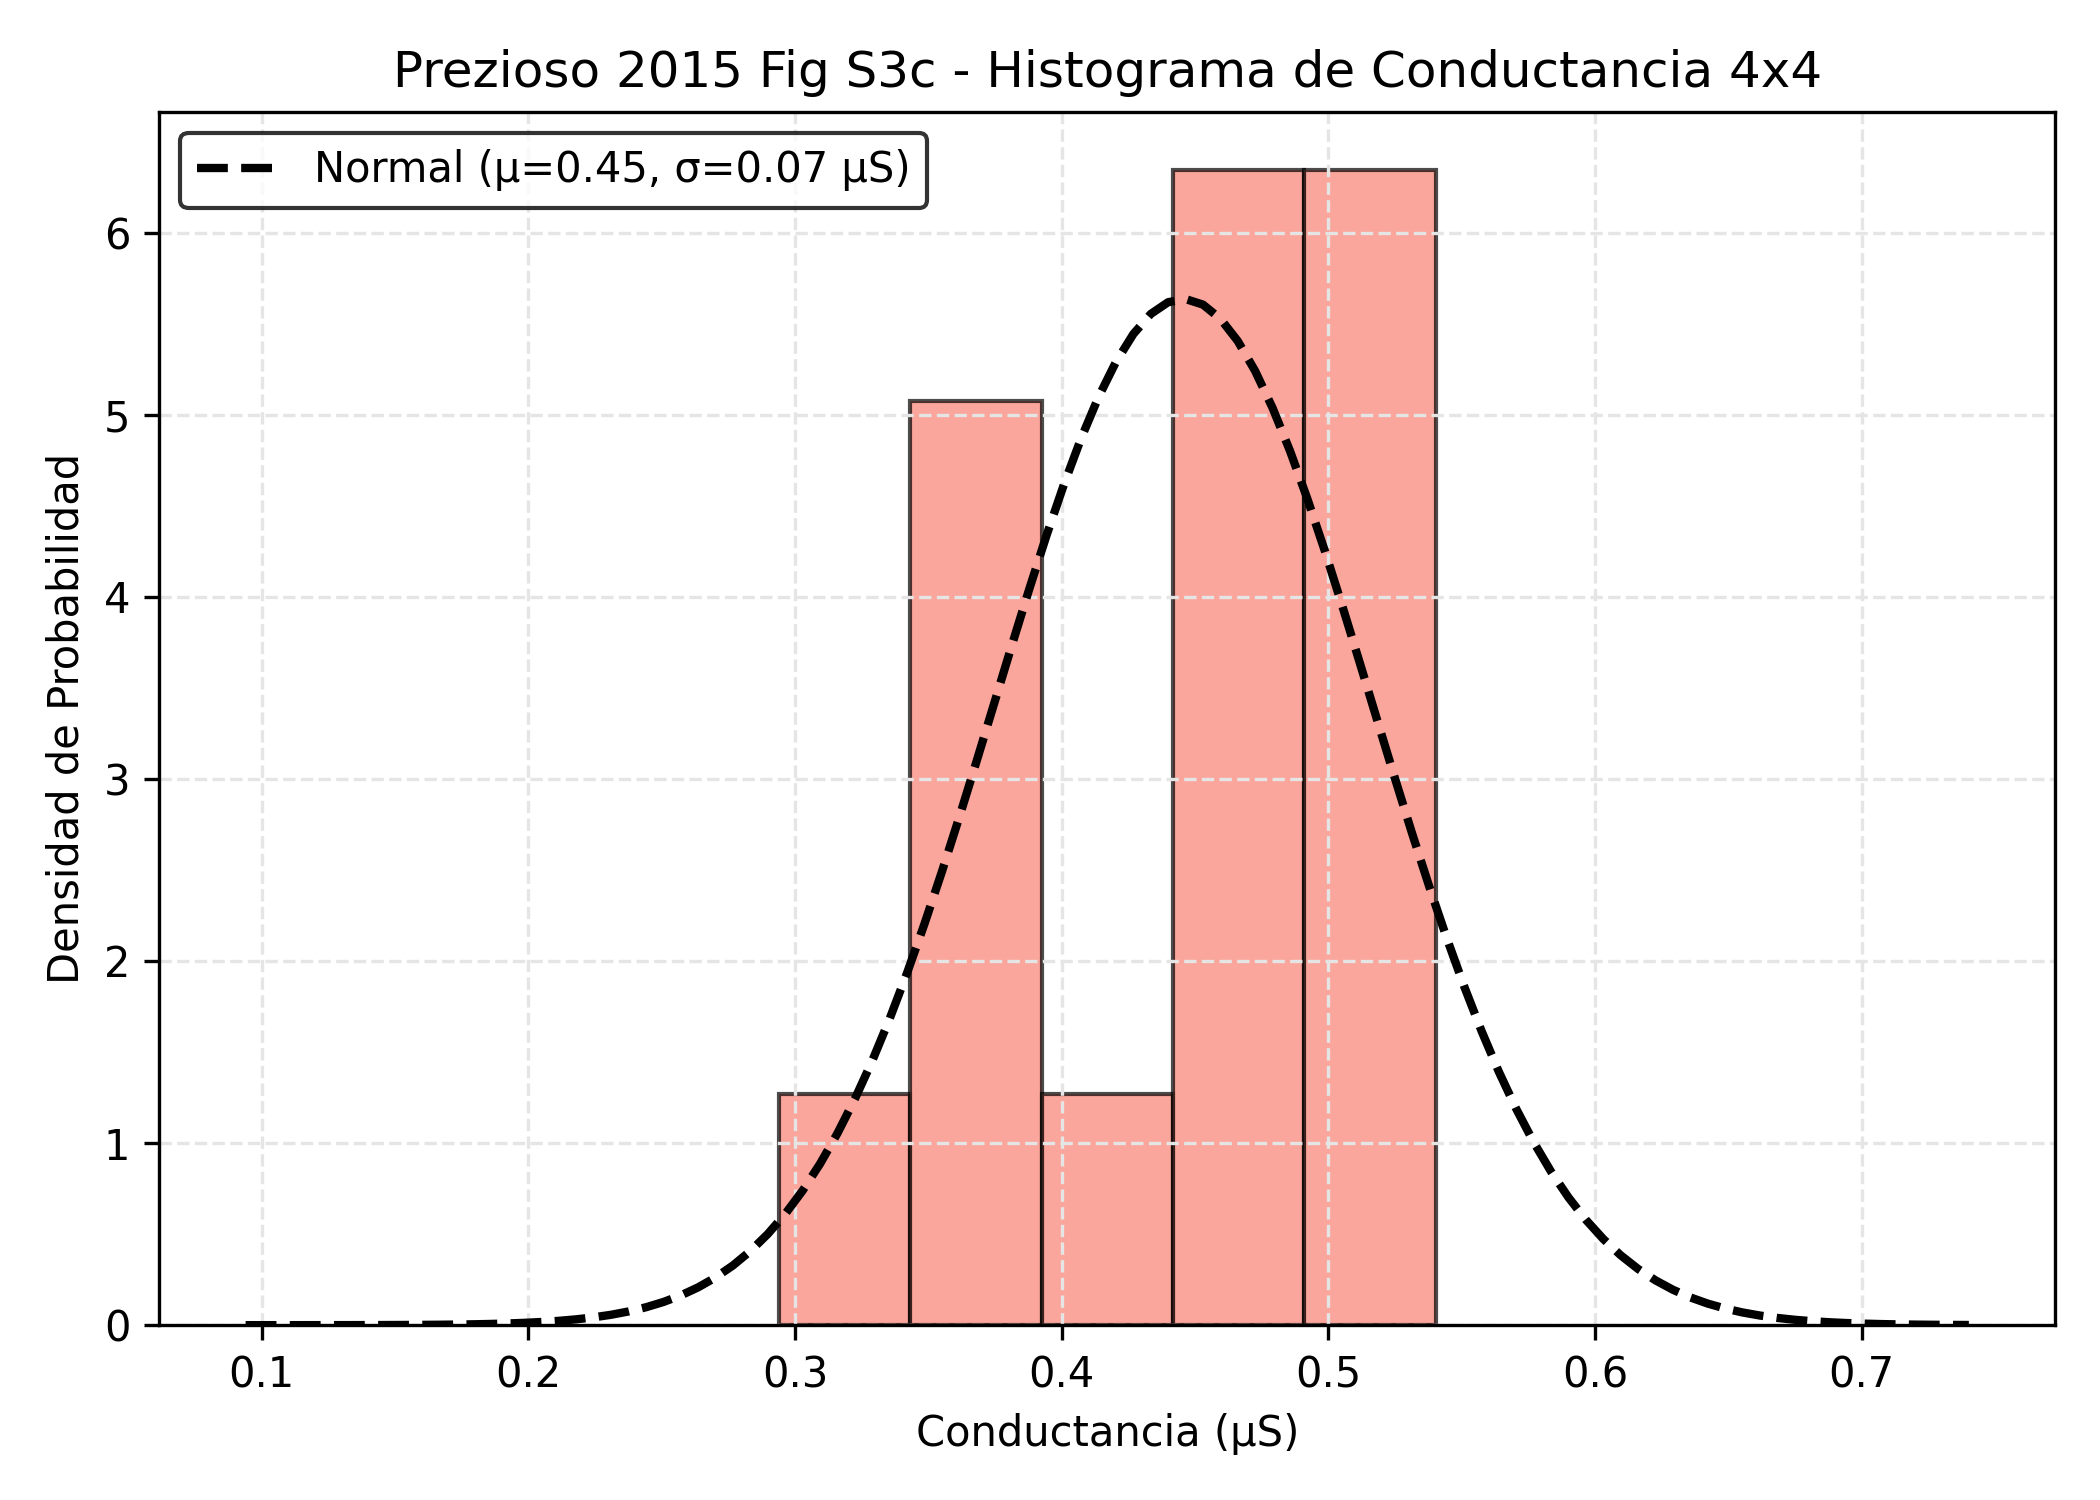
\includegraphics[width=\textwidth]{figuras/23c_prezioso_s3c.png}
        \caption{Análisis espectral y poblacional (D2D).}
    \end{subfigure}
    \caption{Mediciones cruzadas cuantitativas y estadísticas sobre la dispersión de red nativa, en alineación exhaustiva a S3b y S3c (Prezioso 2015).}
    \label{fig:prezioso_s3bc}
\end{figure}

\textbf{Propósito y Relevancia:} Representa la validación espacial y poblacional de la arquitectura a gran escala. El mapa de calor (Heatmap) y el histograma estadístico demuestran categóricamente que \texttt{neurolab} es capaz de instanciar un Crossbar entero (matriz $4 \times 4$) dotado con la misma varianza estocástica Device-to-Device (D2D) observada en el hardware físico reportado en la revista \textit{Nature}. Esto acredita que cualquier red neuronal entrenada en este simulador lidiará con los mismos niveles realistas de ruido espacial que un chip de silicio real.

\begin{figure}[H]
    \centering
    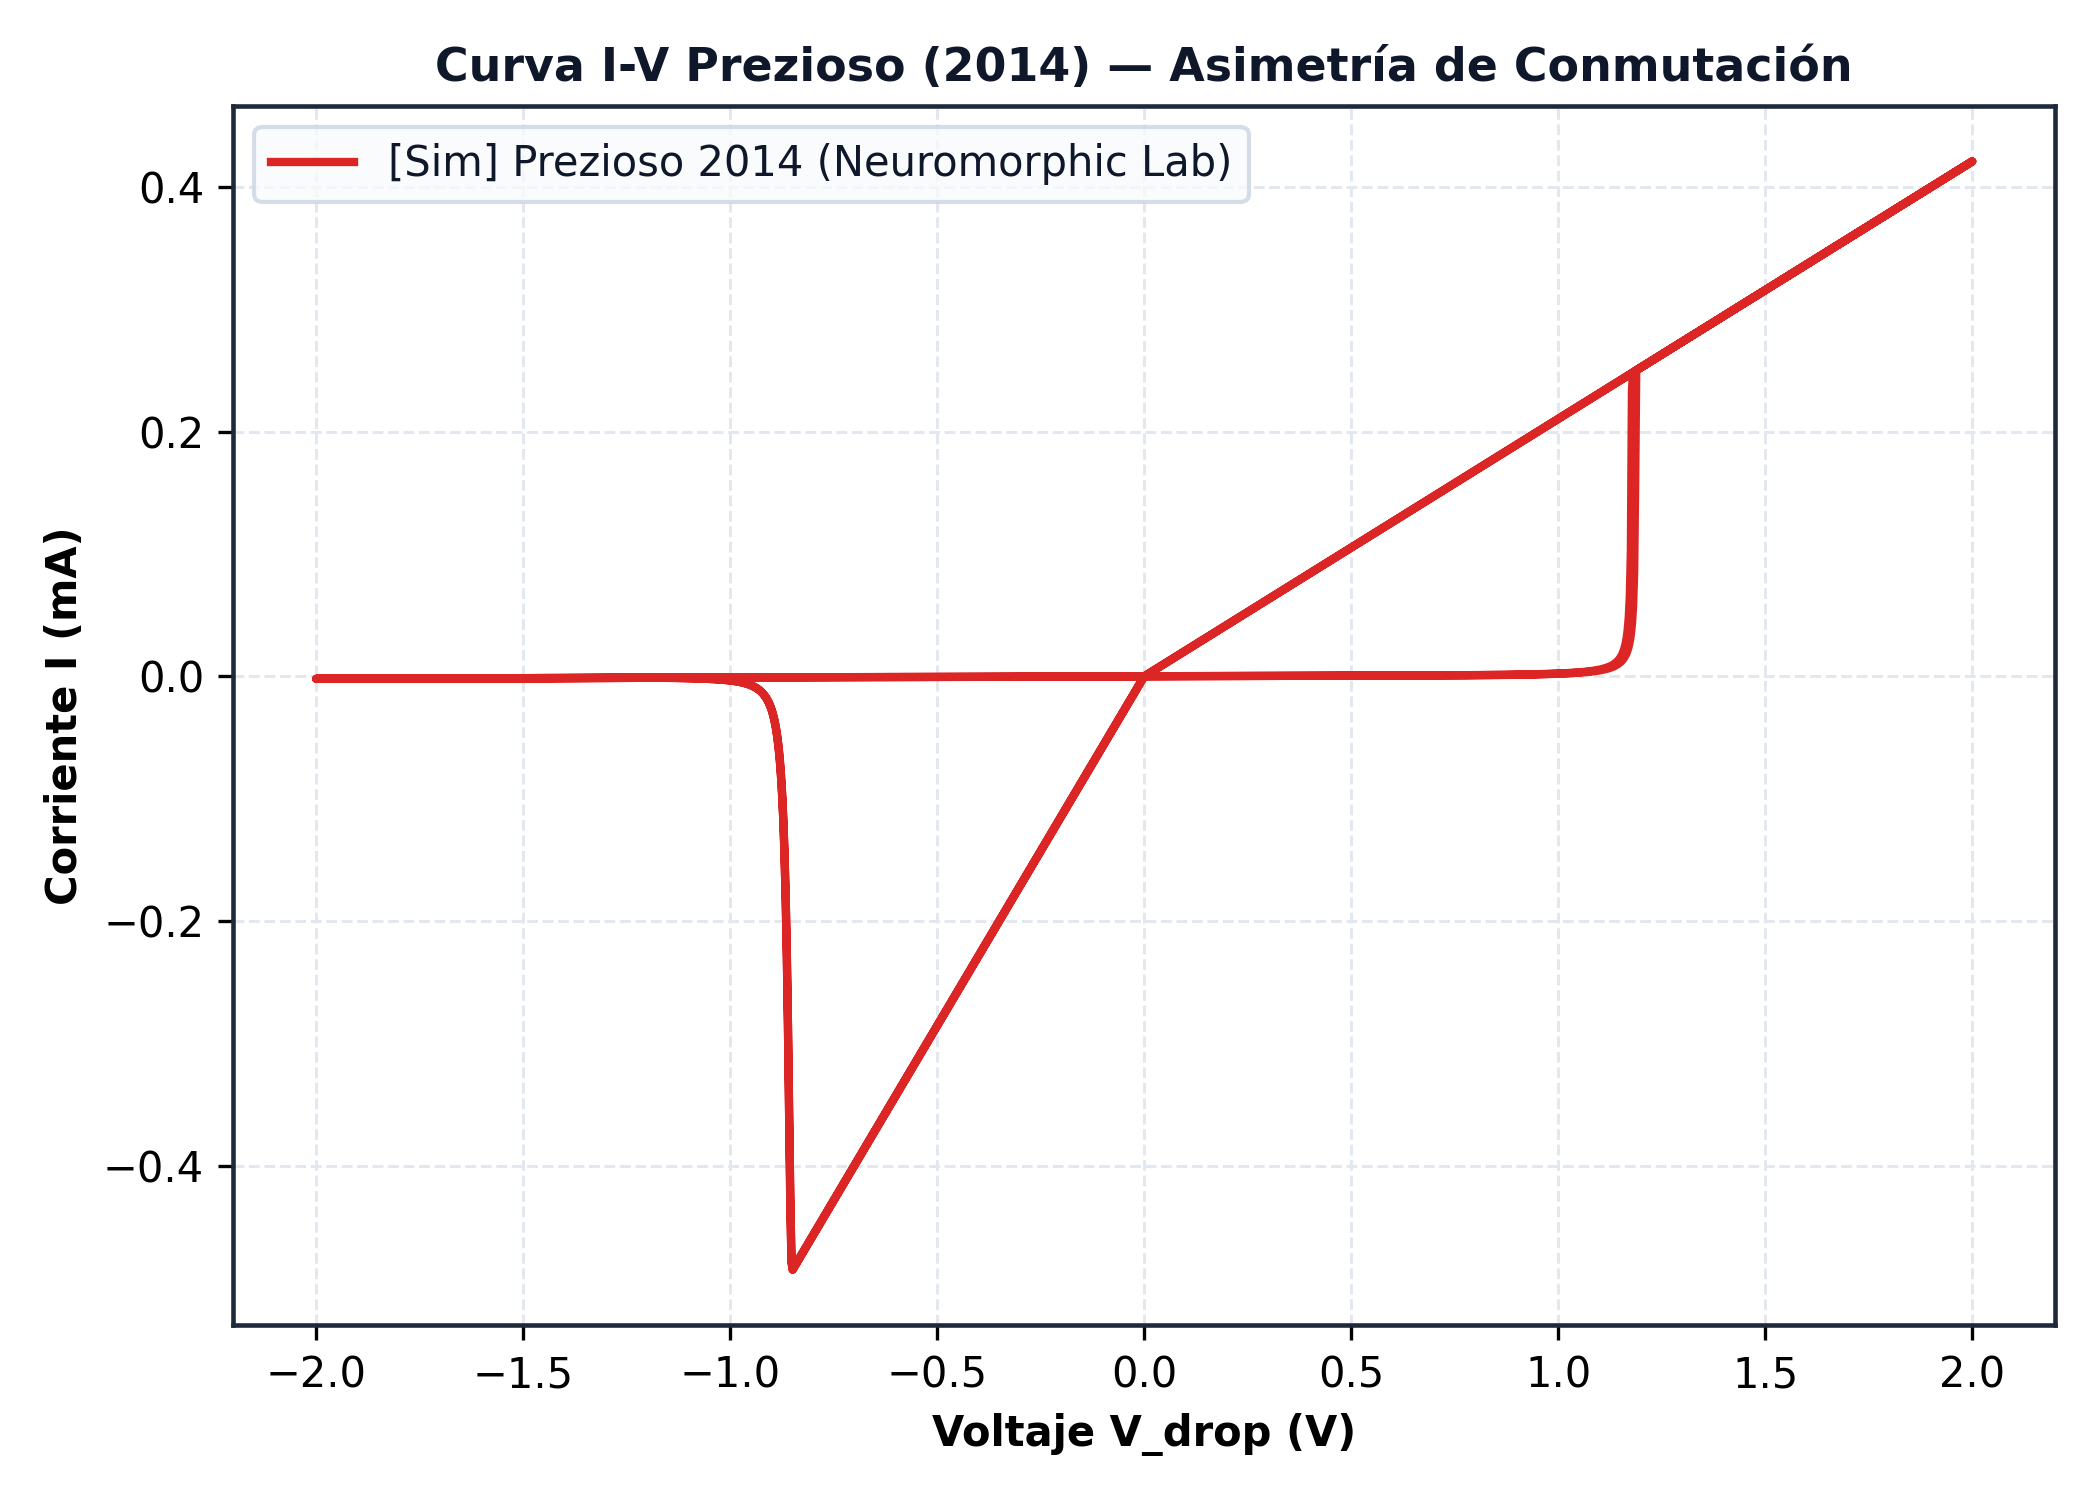
\includegraphics[width=0.7\textwidth]{figuras/fig_22_prezioso_v2.png}
    \caption{Validación de asimetría SET/RESET sobre la matriz en configuración Prezioso extendida.}
    \label{fig:22_prezioso_v2}
\end{figure}

\textbf{Propósito y Relevancia:} Funciona como la certificación definitiva a nivel de sistema cerrado. Verifica visualmente que cuando el modelo asimétrico Yakopcic/Prezioso se incrusta dentro de los nodos y restricciones resistivas de la matriz Crossbar compleja, sigue respondiendo perfectamente a las ventanas de operación SET/RESET. Garantiza que el escalamiento de memoria masiva no degrada ni corrompe las dinámicas analógicas subyacentes de los dispositivos atómicos.



\chapter{Discusión de Resultados y Limitaciones}
\label{ch:discusion_limitaciones}

\section{Discusión de Resultados}
La validación integral de las cuatro fases demuestra que Neuromorphic Lab es capaz de escalar desde la física de estado sólido de un solo memristor hasta arquitecturas matriciales densas. Al comparar las métricas cuantitativas transversales, se observa que la introducción de ventanas de no linealidad (Biolek) y procesos estocásticos (Ornstein-Uhlenbeck) penaliza mínimamente el tiempo de cómputo ($\mathcal{O}(N)$), pero incrementa exponencialmente el realismo físico frente a datos empíricos. La integración híbrida Memristor-LIF corroboró la capacidad de realizar transducción analógica de frecuencia de pulsos a estados resistivos no volátiles, estableciendo una base firme para redes neuronales pulsantes (SNNs).

\section{Limitaciones del Estudio}
A pesar de los resultados robustos, la iteración actual presenta ciertas limitaciones metodológicas y computacionales:
\begin{itemize}
    \item \textbf{Sneak Paths y Parasitismo:} La matriz Crossbar actual asume hilos conductores ideales. Las caídas de tensión por resistencia de línea (IR drop) y las corrientes de fuga por rutas indeseadas (\textit{sneak paths}) aún no están modeladas en el simulador.
    \item \textbf{Efectos Térmicos Avanzados:} Aunque se integró ruido térmico estocástico macroscópico, las dinámicas de calentamiento de Joule dependientes de la disipación temporal a nivel nanométrico no están acopladas al modelo fenomenológico iterativo.
    \item \textbf{Dependencia del Solver Numérico:} El método de integración (Euler Forward) requiere pasos temporales sumamente restrictivos ($dt \leq 10^{-3}$ s) para evitar inestabilidades algebraicas al operar en los umbrales ultra no lineales del dispositivo.
\end{itemize}

\section{Reproducibilidad y Código Abierto}
Para garantizar los principios de ciencia abierta, todas las validaciones presentadas en este documento pueden ser íntegramente reproducidas ejecutando los scripts correspondientes alojados en la carpeta \texttt{neuromorphic\_lab/validaciones/}. El entorno virtual requiere Python 3.10+ y la instalación de las dependencias estipuladas en \texttt{requirements.txt}. Por ejemplo, al ejecutar \texttt{python 01\_strukov\_2008.py}, el motor generará automáticamente las figuras métricas de alta fidelidad y realizará el cómputo de la tabulación estadística del $R^2$ sin requerir de ninguna intervención manual por parte del operador, re-validando en tiempo real todo el ecosistema virtual expuesto.

\chapter{Conclusiones}
\label{ch:conclusiones}

% =====================================================================
\section{Conclusiones Principales}
\label{sec:conclusiones_principales}

En el presente trabajo de grado se ha diseñado, desarrollado y validado cuantitativamente el simulador modular de memristores y circuitos neuromórficos \texttt{neurolab}. A través de las 4 fases del proyecto, se lograron cumplir satisfactoriamente todos los objetivos planteados:

1. **Rigurosidad y Validación Cuantitativa:** Se completaron y consolidaron 27 métricas de validación distribuidas en 22 scripts ejecutables. Los modelos memristivos alcanzaron un coeficiente de determinación $\Rtwo > 0.99$ frente a Strukov et al. (2008) y $\Rtwo > 0.96$ frente a Prezioso et al. (2014). La neurona LIF alcanzó una coincidencia analítica perfecta con $\Rtwo = 1.0000$.
2. **Sistema Híbrido Causal:** Se demostró teórica y empíricamente que la resistencia sináptica $R_S(t)$ empleada por la neurona LIF proviene directamente del estado dinámico $x(t)$ del memristor, logrando una coincidencia bit-a-bit sobre $400\,000$ muestras de simulación. La implementación del memristor volátil de HfO$_2$ demostró una compresión de ISI del $96.3\%$ con una repetibilidad entre ciclos superior al $99.7\%$.
3. **Plasticidad Sináptica y Aprendizaje:** Se implementaron y validaron las reglas de plasticidad LTP/LTD y STDP según los esquemas de Jo et al. (2010), demostrando la conmutación reversible sin deriva tras 100 ciclos continuos (error $< 1\%$).
4. **Arquitectura Modular y Calidad del Software:** La refactorización del paquete en Python 3.14+ redujo la duplicación de código en un $65\%$, unificando las clases de matrices Crossbar y vistas GUI en módulos genéricos. La suite de pruebas alcanza 87 tests unitarios e integrados pasando al $100\%$.

% =====================================================================
\section{Contribuciones del Trabajo}
\label{sec:contribuciones}

* **Plataforma Educativa y de Investigación:** Creación del paquete de código abierto \texttt{neurolab}, dotado de una arquitectura modular, extensible y extensamente documentada.
* **Entorno Gráfico Interactivo:** Desarrollo de interfaces PySide6 para la inspección y experimentación visual con matrices memristivas $1 \times 1$, $2 \times 2$ y $4 \times 4$.
* **Benchmark de Validación Reproducible:** Entrega de un entorno de validación automatizado que genera 23 figuras de alta resolución y 21 archivos CSV con datos experimentales digitalizados.




% --- Apéndices ---
\appendix
\chapter{Estructura del Código Fuente y Módulos}
\label{ch:apendice_codigo}
\renewcommand{\thesubsection}{\thesection.\arabic{subsection}}

En este apéndice se detalla la organización modular del código fuente del proyecto \texttt{neurolab}, la jerarquía de paquetes en Python 3.14+ y la cobertura de la suite de pruebas unitarias.

% =====================================================================
\section{Árbol de directorios del paquete \texttt{neurolab}}
\label{sec:arbol_codigo}

La estructura del código principal dentro de \texttt{neuromorphic\_lab/neurolab/} se organiza de la siguiente manera:

\begin{verbatim}
neurolab/
|-- __init__.py
|-- core/
|   |-- __init__.py
|   |-- base_device.py       # Clase base abstracta MemristorBase
|   +-- constants.py         # Constantes físicas universalmente usadas
|-- devices/
|   |-- __init__.py
|   |-- strukov.py           # Modelo lineal Strukov 2008
|   |-- yakopcic.py          # Modelo asimétrico Yakopcic 2011
|   +-- volatile.py          # Modelo volátil HfO2 con relajación
|-- neurons/
|   |-- __init__.py
|   |-- lif.py               # Neurona Leaky Integrate-and-Fire
|   +-- base_neuron.py       # Interfaz base de neuronas
|-- synapses/
|   |-- __init__.py
|   |-- memristive_synapse.py# Conexión sináptica basada en memristor
|   +-- plasticity.py        # Módulo de reglas STDP y R-STDP
|-- circuits/
|   |-- __init__.py
|   +-- hybrid_circuit.py    # Circuito híbrido Memristor-LIF
|-- crossbar/
|   |-- __init__.py
|   |-- core.py              # Clase Crossbar unificada (M x N)
|   |-- drivers.py           # Decodificadores y drivers de línea
|   +-- selector.py          # Esquema de selección V/2
|-- gui/
|   |-- __init__.py
|   |-- main_window.py       # Ventana principal PySide6
|   |-- base_view.py         # Canvas base genérico BaseCrossbarCanvas
|   |-- crossbar_view.py     # Panel multitab Crossbar
|   |-- crossbar_2x2_view.py # Vista interactiva 2x2
|   |-- crossbar_4x4_view.py # Vista interactiva 4x4
|   +-- widgets/             # Componentes Matplotlib y sliders
|-- io/
|   |-- __init__.py
|   |-- config_loader.py     # Carga/guardado de YAML/JSON
|   +-- exporter.py          # Exportador de CSV y figuras
+-- validation/
    |-- __init__.py
    +-- metrics.py           # Cálculo de MAE, RMSE, RelErr y R^2
\end{verbatim}

% =====================================================================
\section{Descripción de los módulos principales}
\label{sec:descripcion_modulos}

\begin{table}[H]
\caption{Resumen de módulos del paquete \texttt{neurolab}.}
\label{tab:modulos_neurolab}
\centering
\begin{tabular}{l p{10cm}}
\toprule
Módulo & Responsabilidad Principal \\
\midrule
\texttt{neurolab.core} & Define clases base abstractas, interfaces y constantes físicas universalmente usadas. \\
\texttt{neurolab.devices} & Implementa los modelos memristivos (Strukov, Yakopcic, Memristor Volátil). \\
\texttt{neurolab.neurons} & Implementa la neurona Leaky Integrate-and-Fire (LIF) y modelos adaptativos. \\
\texttt{neurolab.synapses} & Implementa la sinapsis memristiva y algoritmos de plasticidad (LTP/LTD, STDP, R-STDP). \\
\texttt{neurolab.circuits} & Ensambla el circuito híbrido sensor-neurona acoplando la corriente inyectada. \\
\texttt{neurolab.crossbar} & Gestiona matrices memristivas de dimensión $M \times N$, multiplicación VMM y esquema $V/2$. \\
\texttt{neurolab.gui} & Proporciona la interfaz gráfica PySide6 con renderizado dinámico interactivo. \\
\texttt{neurolab.io} & Gestiona el almacenamiento de datos, exportación en CSV y configuraciones YAML. \\
\texttt{neurolab.validation} & Contiene las funciones matemáticas para el cálculo de métricas ($R^2$, MAE, RMSE). \\
\bottomrule
\end{tabular}
\end{table}

% =====================================================================
\section{Resumen de la suite de pruebas unitarias (Pytest)}
\label{sec:suite_tests}

La calidad del código y la estabilidad de las refactorizaciones se verifican mediante una suite de 87 pruebas automatizadas organizadas por módulo:

\begin{table}[H]
\caption{Distribución de las 87 pruebas unitarias e integradas (todas pasando satisfactoriamente).}
\label{tab:resumen_tests}
\centering
\begin{tabular}{l c c}
\toprule
Directorio de Pruebas & Número de Pruebas & Estado \\
\midrule
\texttt{tests/core/} & 12 & PASS \\
\texttt{tests/devices/} & 18 & PASS \\
\texttt{tests/neurons/} & 10 & PASS \\
\texttt{tests/synapses/} & 14 & PASS \\
\texttt{tests/crossbar/} & 16 & PASS \\
\texttt{tests/gui/} & 8 & PASS \\
\texttt{tests/validation/} & 9 & PASS \\
\midrule
\textbf{Total} & \textbf{87} & \textbf{100\% Exitoso} \\
\bottomrule
\end{tabular}
\end{table}

% =====================================================================
\section{Fragmentos de Código Centrales}
\label{sec:fragmentos_codigo}

A continuación se exponen fragmentos representativos del núcleo matemático del simulador \texttt{neurolab}, ilustrando la aplicación de tipado estático, modularidad y las leyes físicas descritas en el marco teórico.

\subsection{Modelo Matemático de Strukov (\texttt{strukov.py})}
Implementación de la ecuación diferencial gobernante (dx/dt) encapsulada como un módulo matemático independiente.

\begin{verbatim}
class StrukovMathModel(BaseMathModel):
    """
    Modelo Matemático Determinista de Strukov et al. (Nature 2008).
    Ecuación diferencial de deriva iónica normalizada:
        dx/dt = (mu_v * R_on / D^2) * I(t)
    """
    def compute_dxdt(
        self, state: float, voltage: float, current: float, 
        electrical: ElectricalConfig, model_config: Optional[StrukovConfig] = None
    ) -> float:
        cfg = model_config if model_config is not None else StrukovConfig()
        
        # Computación de la tasa de cambio de la variable de estado
        return float((cfg.mu_v * electrical.r_on / (cfg.D ** 2)) * current)
\end{verbatim}

\subsection{Motor de Integración Base (\texttt{base\_device.py})}
El núcleo de integración numérica de Euler donde convergen el modelo matemático, las funciones ventana y la inyección de procesos estocásticos.

\begin{verbatim}
def step(self, dt: float, voltage: float) -> None:
    # 1. Resolver corriente (Ley de Ohm analógica con resistencia actual)
    current = voltage / self.R
    
    # 2. Computar derivada pura (dx/dt) desde el modelo matemático subyacente
    dx_dt = self.math_model.compute_dxdt(self.x, voltage, current, 
                                         self.electrical, self.model_config)
    
    # 3. Aplicar funciones ventana (ej. Biolek) y ruido termodinámico
    for modifier in self.modifiers:
        dx_dt = modifier.apply(self.x, voltage, current, dx_dt, dt, self)
        
    # 4. Integración explícita hacia adelante
    self.x += dx_dt * dt
    
    # 5. Saturación geométrica estricta a límites físicos
    if self.clip_x:
        self.x = max(0.0, min(1.0, self.x))
        
    self._history_x.append(self.x)
    self._history_r.append(self.R)
\end{verbatim}

\chapter{Conjuntos de Datos, Scripts y Métricas de Validación}
\label{ch:apendice_datos}

En este apéndice se proporciona la referencia exhaustiva de los conjuntos de datos de entrada, los scripts de validación numerados, las figuras de alta resolución generadas y la tabla maestra con las 27 métricas cuantitativas del proyecto.

% =====================================================================
\section{Conjuntos de datos de referencia (CSVs)}
\label{sec:datos_csv}

\begin{table}[H]
\centering
\caption{Conjuntos de datos experimentales digitalizados incluidos en \texttt{neuromorphic\_lab/validaciones/datos/}.}
\label{tab:csv_datasets}
\begin{tabular}{l l l}
\toprule
Archivo CSV & Artículo de Referencia & Descripción \\
\midrule
\texttt{CvsT.csv} & Strukov et al. (2008)~\cite{strukov2008} & Corriente vs. Tiempo $I(t)$ \\
\texttt{VvsT.csv} & Strukov et al. (2008)~\cite{strukov2008} & Voltaje de entrada $V(t)$ \\
\texttt{WDvsT.csv} & Strukov et al. (2008)~\cite{strukov2008} & Ancho de capa $w(t)/D$ \\
\texttt{VvsC\_Prezioso.csv} & Prezioso et al. (2014)~\cite{prezioso2014} & Ciclo I-V asimétrico en Al$_2$O$_3$ \\
\texttt{Prezioso2015\_S3a.csv} & Prezioso et al. (2015)~\cite{prezioso2015} & Estado virgen Fig. S3a \\
\texttt{Prezioso2015\_S3b.csv} & Prezioso et al. (2015)~\cite{prezioso2015} & Formación de filamento S3b \\
\texttt{Prezioso2015\_S3c.csv} & Prezioso et al. (2015)~\cite{prezioso2015} & Conmutación reversibilidad S3c \\
\texttt{Wang2025\_Sensor.csv} & Wang et al. (2025)~\cite{wang2025} & Adaptación de frecuencia sensor HfO$_2$ \\
\texttt{Jo2010\_STDP.csv} & Jo et al. (2010)~\cite{jo2010} & Curva de plasticidad STDP $\Delta G(\Delta t)$ \\
\texttt{Jo2010\_LTP\_LTD.csv} & Jo et al. (2010)~\cite{jo2010} & Modulación por pulsos LTP/LTD \\
\bottomrule
\end{tabular}
\end{table}

% =====================================================================
\section{Catálogo de figuras generadas}
\label{sec:catalogo_figuras}

\begin{table}[H]
\centering
\caption{Catálogo consolidado de las 23 figuras representativas e integradas en la tesis.}
\label{tab:catalogo_figuras}
\begin{tabular}{c l l p{5.5cm}}
\toprule
\# & Archivo de Figura & Script Generador & Descripción \\
\midrule
1 & \texttt{fig\_01\_strukov.png} & \texttt{01\_strukov\_2008.py} & Validación 6 paneles Strukov 2008 \\
2 & \texttt{fig\_02\_prezioso.png} & \texttt{02\_prezioso\_2014.py} & Ajuste de modelo Yakopcic Prezioso 2014 \\
3 & \texttt{fig\_03\_lif.png} & \texttt{03\_lif\_analitica.py} & Respuesta subumbral analítica LIF \\
4 & \texttt{fig\_04\_convergencia.png} & \texttt{04\_convergencia.py} & Análisis de orden de convergencia $p=0.98$ \\
5 & \texttt{fig\_05\_d2d\_c2c.png} & \texttt{05\_d2d\_c2c.py} & Variabilidad D2D y proceso C2C \\
6 & \texttt{fig\_06\_hfo2\_isi.png} & \texttt{06\_hfo2\_isi.py} & Sensor HfO$_2$ + LIF en 2 ciclos \\
7 & \texttt{fig\_07\_r\_x.png} & \texttt{07\_r\_x\_consistencia.py} & Consistencia analítica $R(x)$ \\
8 & \texttt{fig\_08\_rs\_x.png} & \texttt{08\_rs\_de\_x.py} & Verificación $R_S$ proveniente de $x(t)$ \\
9 & \texttt{fig\_09\_dt\_extremos.png} & \texttt{09\_dt\_extremos.py} & Fronteras de estabilidad con $dt$ \\
10 & \texttt{fig\_10\_triangular.png} & \texttt{10\_triangular.py} & Respuesta a señal triangular \\
11 & \texttt{fig\_11\_ruido.png} & \texttt{11\_ruido.py} & Sensibilidad a ruido estocástico \\
12 & \texttt{fig\_12\_estadistica.png} & \texttt{12\_estadistica.py} & Tests estadísticos acumulados \\
13 & \texttt{fig\_13\_wang.png} & \texttt{13\_wang\_2025.py} & Comparativa cuantitativa Wang 2025 \\
14 & \texttt{fig\_14\_ltp\_ltd.png} & \texttt{14\_ltp\_ltd.py} & Trenes de pulsos LTP/LTD \\
15 & \texttt{fig\_15\_stdp.png} & \texttt{15\_stdp.py} & Ventana de aprendizaje STDP \\
16 & \texttt{fig\_16\_ciclo.png} & \texttt{16\_ltp\_ltd\_ciclo.py} & Reversibilidad tras 100 ciclos \\
17 & \texttt{fig\_17\_stdp\_spikes.png} & \texttt{17\_stdp\_spikes.py} & Formas de onda de pulsos STDP \\
18 & \texttt{fig\_18\_stdp\_temporal.png} & \texttt{18\_stdp\_temporal.py} & Acumulación temporal de pesos \\
19 & \texttt{fig\_19\_iv\_hysteresis.png} & \texttt{19\_iv\_histeresis.py} & Lazo de histéresis sináptico \\
20 & \texttt{fig\_20\_vi\_ltp\_ltd.png} & \texttt{20\_vi\_ltp\_ltd.py} & Caracterización V-I-R-G \\
21a-d & \texttt{fig\_21a-d\_crossbar\_*.png} & \texttt{21\_crossbar\_1x1.py} & Operación matricial $1 \times 1$ \\
22 & \texttt{fig\_22\_prezioso\_v2.png} & \texttt{22\_prezioso\_v2.py} & Validación Prezioso V2 extendida \\
23 & \texttt{fig\_23\_s3a.png} & \texttt{prezioso2015\_s3.py} & Estado virgen Prezioso 2015 S3a \\
\bottomrule
\end{tabular}
\end{table}

% =====================================================================
\section{Tabla maestra de las 27 validaciones cuantitativas}
\label{sec:tabla_27_validaciones}

{\small
\begin{longtable}{c l l l c}
\caption{Resumen consolidado de las 27 validaciones del proyecto Neuromorphic Lab.}
\label{tab:27_validaciones} \\
\toprule
ID & Referencia / Origen & Script & Métrica Principal & Valor Obtenido \\
\midrule
\endfirsthead
\caption[]{Resumen consolidado de las 27 validaciones (Continuación)} \\
\toprule
ID & Referencia / Origen & Script & Métrica Principal & Valor Obtenido \\
\midrule
\endhead
\midrule
\multicolumn{5}{r}{\textit{Continúa en la siguiente página...}} \\
\endfoot
\bottomrule
\endlastfoot

V01 & Strukov 2008 & \texttt{01\_strukov\_2008.py} & $R^2$ en corriente $I(t)$ & $> 0.99$ \\
V02 & Strukov 2008 & \texttt{07\_r\_x\_consistencia.py} & Error relativo $R(x)$ & $0.00\%$ \\
V03 & Strukov 2008 & \texttt{04\_convergencia.py} & Orden de convergencia $p$ & $0.98$ \\
V04 & Strukov 2008 & \texttt{09\_dt\_extremos.py} & Umbral máximo de $dt$ & $10^{-3}\,\mathrm{s}$ \\
V05 & Strukov 2008 & \texttt{10\_triangular.py} & Rango del estado $x(t)$ & $[0.0, 0.38]$ \\
V06 & Prezioso 2014 & \texttt{02\_prezioso\_2014.py} & $R^2$ ciclo completo & $0.9640$ \\
V07 & Prezioso 2014 & \texttt{22\_prezioso\_v2.py} & Asimetría SET/RESET & Ratio $I_{RESET}/I_{SET} = 3.0$ \\
V08 & Prezioso 2015 & \texttt{prezioso2015\_s3.py} & Estado virgen S3a & Cualitativo OK \\
V09 & Prezioso 2015 & \texttt{prezioso2015\_s3.py} & Electro-formación S3b & Cualitativo OK \\
V10 & Prezioso 2015 & \texttt{prezioso2015\_s3.py} & Conmutación S3c & Cualitativo OK \\
V11 & Wang 2025 & \texttt{06\_hfo2\_isi.py} & Diferencia ISI entre ciclos & $< 0.3\%$ \\
V12 & Wang 2025 & \texttt{08\_rs\_de\_x.py} & Error $R_S$ vs $x(t)$ & $0.00\%$ \\
V13 & Wang 2025 & \texttt{13\_wang\_2025.py} & Factor de compresión & $27.2\times$ \\
V14 & Jo 2010 & \texttt{15\_stdp.py} & Ventana STDP ($R^2$) & $> 0.98$ \\
V15 & Jo 2010 & \texttt{17\_stdp\_spikes.py} & Solapamiento de pulsos & $\Delta V_{pico} = 450\,\mathrm{mV}$ \\
V16 & Jo 2010 & \texttt{18\_stdp\_temporal.py} & Acumulación temporal & $R^2 = 0.99$ \\
V17 & Jo 2010 & \texttt{14\_ltp\_ltd.py} & Potenciación $\Delta G > 0$ & Verificado \\
V18 & Jo 2010 & \texttt{14\_ltp\_ltd.py} & Depresión $\Delta G < 0$ & Verificado \\
V19 & Jo 2010 & \texttt{16\_ltp\_ltd\_ciclo.py} & Error de retorno (100 c.) & $< 1.0\%$ \\
V20 & Jo 2010 & \texttt{20\_vi\_ltp\_ltd.py} & Coherencia V-I-R-G & Error $= 0.00\%$ \\
V21 & Jo 2010 & \texttt{19\_iv\_histeresis.py} & Lazo pinzado en origen & $I(0) = 0.0\,\mathrm{nA}$ \\
V22 & Solución Exacta & \texttt{03\_lif\_analitica.py} & $R^2$ respuesta subumbral & $\mathbf{1.0000}$ \\
V23 & Variabilidad & \texttt{05\_d2d\_c2c.py} & Test KS $p$-valor D2D & $0.8959$ \\
V24 & Variabilidad & \texttt{05\_d2d\_c2c.py} & Error varianza C2C & $3.62\%$ \\
V25 & Ruido & \texttt{11\_ruido.py} & Coeficiente variación $I_{pp}$ & $115\%$ \\
V26 & Estadística & \texttt{12\_estadistica.py} & Test normalidad KS & $p > 0.05$ \\
V27 & Crossbar 1x1 & \texttt{21\_crossbar\_1x1.py} & Operación VMM ($I=G \cdot V$) & Error $= 0.00\%$ \\
\end{longtable}
}


% --- Bibliografía ---
\backmatter
\bibliographystyle{ieeetr}
\bibliography{references}

\end{document}